% wfs_chapter_hda
% repository https://github.com/spatialaudio/wfs_chapter_hda
% authors:
% - Frank Schultz, https://orcid.org/0000-0002-3010-0294, https://github.com/fs446
% - Nara Hahn, https://orcid.org/0000-0003-3564-5864, https://github.com/narahahn
% - Sascha Spors, https://orcid.org/0000-0001-7225-9992, https://github.com/spors
%
% authors' versions for the chapters (English, German) on **Wave Field Synthesis** in
% - Stefan Weinzierl (editor): *Handbuch der Audiotechnik*, 2nd GER edition, Springer, 2025
% - Stefan Weinzierl (editor): *Handbook of Audio Technology*, 1st ENG edition, Springer, TBA
% - https://link.springer.com/book/10.1007/978-3-662-60369-7
%
% text and graphics under [CC BY 4.0 license](https://creativecommons.org/licenses/by/4.0/)
% source code under [MIT license](https://opensource.org/licenses/MIT)
% publisher Springer has copyright to their finally edited and authors' approved English / German chapters and their layouts
%
% we use the violine image from https://upload.wikimedia.org/wikipedia/commons/thumb/f/f1/Violin.svg/2048px-Violin.svg.png
% to create the files `python/violin_wfs_ENG.png` and `python/violin_wfs_DEU.png`
%
% we use the photo `fotos/WFS_Array_UniRostockH8_2014.jpg` CC BY 4.0 Matthias Geier & Sascha Spors
%
% all other graphics (as pdf, png, eps, svn, ipe) in this repository are CC BY 4.0 Frank Schultz & Nara Hahn
%
% we might also find https://git.iem.at/zotter/wfs-basics useful
%##############################################################################

%\section{Einleitung}
\section{Introduction}
\label{sec:WFSIntro}

%Wellenfeldsynthese (WFS)\index{Wellenfeldsynthese} \cite{Vries2009_Mono, Sporer2018_book}
%ist ein nicht-kanalbasiertes Lautsprecherwiedergabeverfahren, welches in der Praxis
%häufig zur Spatialisierung von Audio-Objekten verwendet wird \cite{Ranjan2013_IEEE}.
Wave field synthesis\index{wave field synthesis} (WFS)\index{WFS}
\cite{Vries2009_Mono, Sporer2018_book} is a non-channel-based loudspeaker
reproduction method that is frequently used in practice for the spatialisation
of audio objects \cite{Ranjan2013_IEEE}.
%
%Mit einer großen Anzahl dicht gereihter und individuell ansteuerbarer Lautsprecher
%werden Überlagerungen von Wellen, d.h. Interferenzen, kontrolliert erzeugt,
%so dass gewünschte Wellenfrontenverläufe\index{Wellenfront}
%entstehen, vgl.~\myfig\ref{fig:violine}~(rechts) und \myfig\ref{fig:td_0m}.
A large number of closely spaced loudspeakers are individually controlled to
generate a desired wavefront\index{wavefront},
cf.~\myfig\ref{fig:violine}~(right) and \myfig\ref{fig:td_0m},
resulting from wave superposition,
i.e. interference.
%Die WFS wird den sogenannten \index{Schallfeldsynthese}Schallfeldsyntheseverfahren
%zugeordnet \cite{Spors2013_IEEE}. % moved to 'initial primary objective' paragraph
%und für Audioanwendungen seit Ende der 1980er Jahre \cite{Berkhout1988_JAES}
%erforscht und entwickelt.
%
The WFS has been researched and developed for audio applications since the late
1980s \cite{Berkhout1988_JAES}.
%
%In der Praxis werden meist horizontale, zuhörerflächen-(teil)-umschließende
%Lautsprecherarrays verwendet, also z.B. Rechteck-, Kreisarrays oder frontale
%Zeilen, vgl.~\myfig\ref{fig:WFS_Array_Haus8} und \cite{Vries2009_Mono, Vries2019}.
In practice, horizontal loudspeaker arrays that (partially) enclose the
listening areas are mainly utilised, e.g. rectangular, circular or frontal linear
arrays, cf. the setup in \myfig\ref{fig:WFS_Array_Haus8} and further examples
in \cite{Vries2009_Mono, Vries2019}.



% please DO NOT rescale the figure and keep it double column
\begin{figure*}
\centering
\begin{plotfigures}
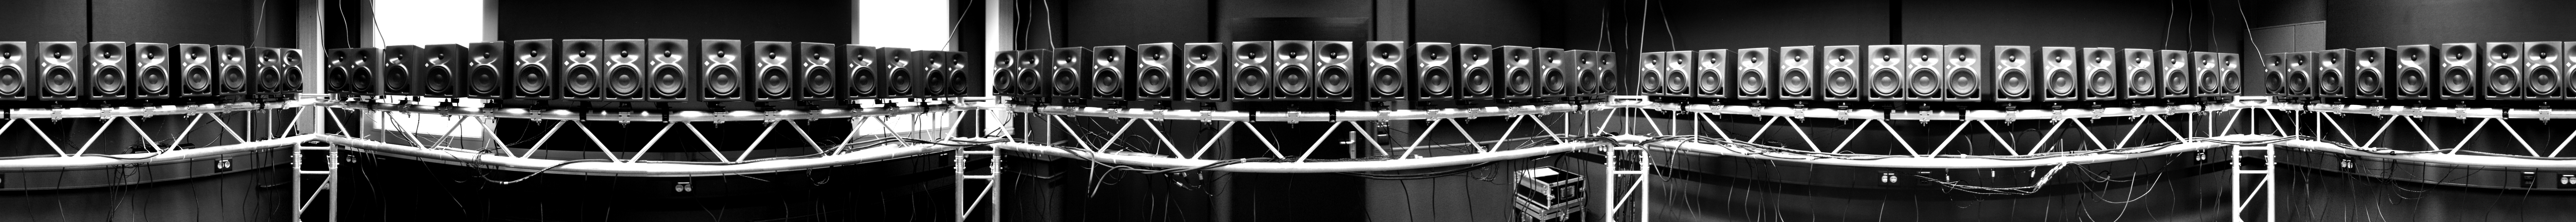
\includegraphics[width=174mm]{../fotos/WFS_Array_UniRostockH8_2014.jpg}
\end{plotfigures}
\caption{%Panoramafoto des WFS-Systems im Audio-Labor der Universität Rostock mit
%64 Zwei-Weg-Studiomonitoren auf Ohrhöhe für mittelgroße, stehende Zuhörende und
%entlang einer $4 \text{m} \times 4 \text{m}$ quadratischen Hüllkontur mit freien
%Ecken und mittlerem Lautsprecherabstand von ca. $0{,}23$\,m.
Panoramic photo of the WFS system in the audio laboratory at the University
of Rostock.
The array contour follows the edges of a $4\,\text{m} \times 4\,\text{m}$
square equipped with 64 two-way studio monitors at ear level for
standing listeners with average height.
The mean loudspeaker spacing is approximately $0{.}23$\,m.
%
CC BY 4.0 Matthias Geier, Sascha Spors.
}
\label{fig:WFS_Array_Haus8}
\end{figure*}



% please DO NOT rescale the figure and keep it single column
\begin{figure}
\centering
\begin{plotfigures}
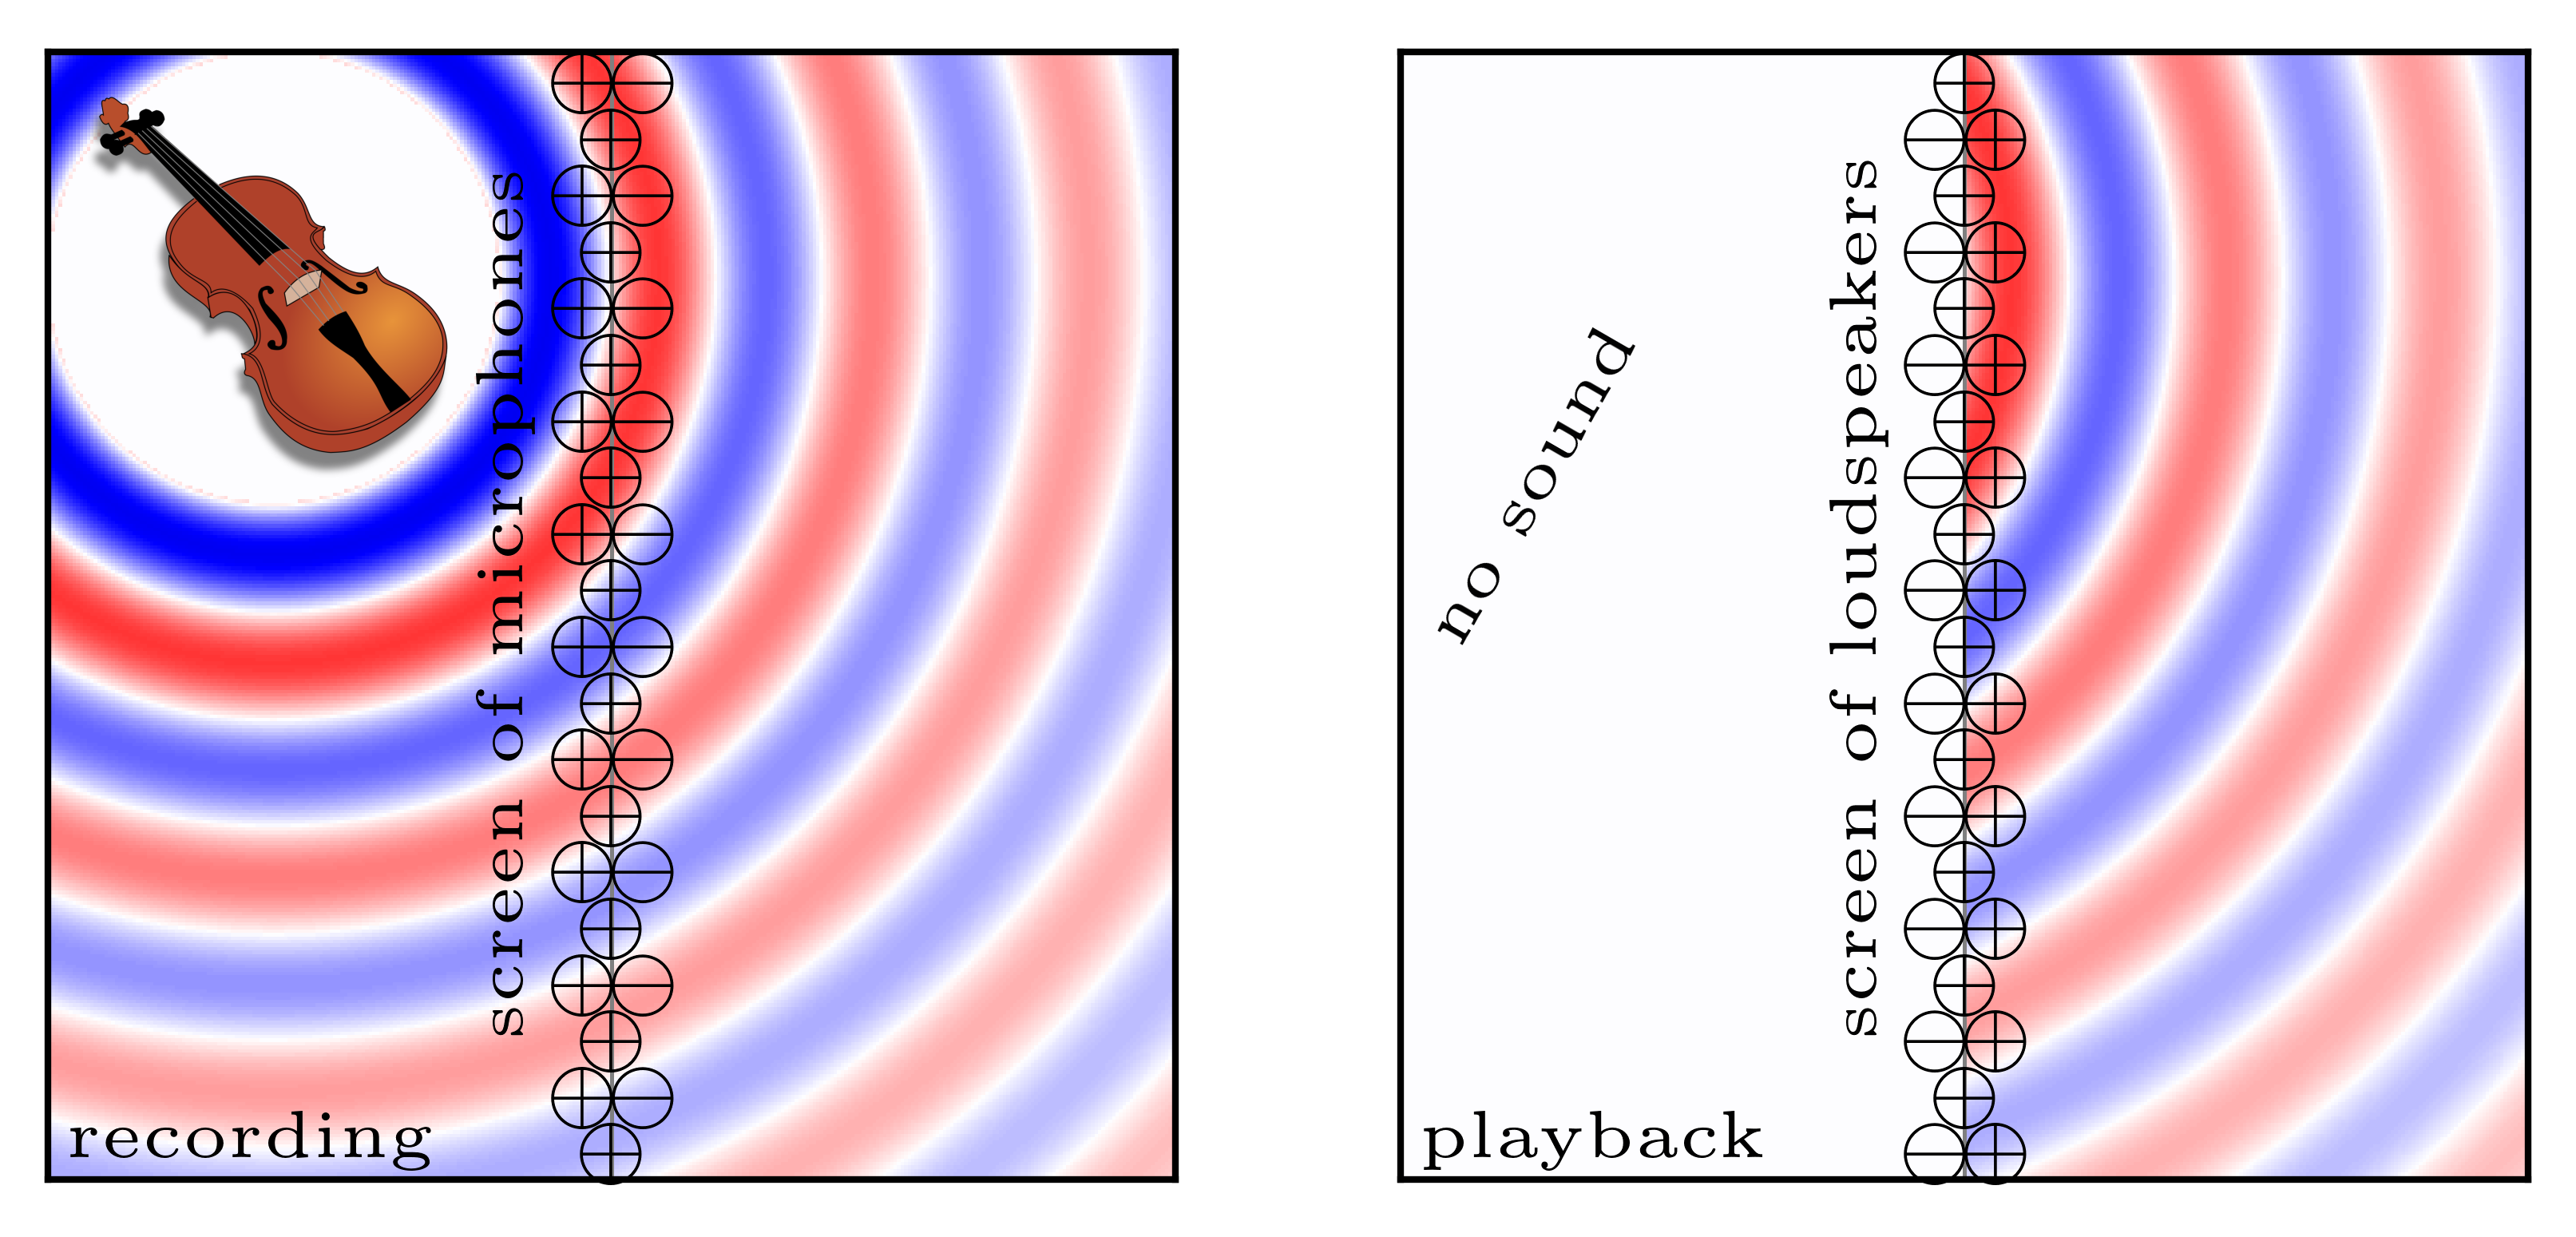
\includegraphics[width=85mm]{../python/violin_wfs_ENG.png}
\end{plotfigures}
\caption{%WFS-Prinzip basierend auf der \myeq\eqref{eq:KHIGeneral} für das
%Halbraumproblem.
WFS principle for the half-space problem.
%
%Links: Aufnahme einer akustischen Szene mit Achter-Druckgradienten-
%$(\oplus\ominus)$ und Druckmikrofonen $(\oplus)$ entlang einer Fläche.
Left: Recording of an acoustic scene with pressure gradient, figure-of-eight
microphones $(\oplus\ominus)$ and pressure microphones $(\oplus)$
set up along a planar surface.
%
%Rechts: die Wiedergabe dieser Signale mit einer Fläche aus
%Monopol- $(\oplus)$ und Dipollautsprechern
%$(\ominus\oplus)$ führt wegen Wellenüberlagerung im
%rechten Halbraum zum gleichen Schallfeld wie das der originalen
%akustischen Szene (datenbasierte Direktwiedergabe).
Right: The reproduction of these signals with a planar array of monopole
loudspeakers $(\oplus)$ and dipole loudspeakers $(\ominus\oplus)$ results
in the same sound field as the original acoustic scene due to wave interference
in the right half-space. This is known as data-based direct reproduction.
%
%Statt Messungen können analytische Schallfeldmodelle
%bezüglich Druck und Druckgradient entlang der Fläche ausgewertet und daraus
%die Ansteuerung für die Lautsprecher berechnet werden
%(modellbasierte Wiedergabe).
Rather than taking measurements, it is possible to calculate
the pressure and the pressure gradient along the surface for
analytical sound field models. These signals can then be used
to derive the driving signals for the loudspeakers. This is
referred to as model-based reproduction.
\cc
}
\label{fig:violine}
\end{figure}



%In diesem Kapitel wird die Grundidee der WFS aufgezeigt.
The purpose of this chapter is to illustrate the fundamental idea of the WFS.
%
%Im Rest dieses Abschnitts wird das WFS-Konzept grundlegend verortet
%und der Wissensstand zur WFS historisch kurz eingeordnet.
The rest of this section provides a basic overview of the WFS concept and
briefly summarises the state of research over time.
%
%In \mych{sec:WFSFundamentals} wird das wellentheoretische Fundament der WFS eingeführt.
In \mych{sec:WFSFundamentals} the wave theory related to WFS is introduced.
%
%Danach wird in \mych{sec:WFS_PointSource} eine kompakte, allgemeine Herleitung
%für die WFS einer virtuellen Punktquelle präsentiert.
Then in \mych{sec:WFS_PointSource} a compact and general derivation for the WFS
of a virtual point source is given.
%
%Mit numerischen Simulationen werden in \mych{sec:WFS_PointSource_Simulationen}
%die wichtigsten Eigenschaften der mit WFS
%erzeugten Schallfelder und einige psychoakustische Implikationen diskutiert.
The most important characteristics of WFS sound fields are discussed in
\mych{sec:WFS_PointSource_Simulationen} by means of numerical simulations.
Major psychoacoustic implications are discussed.
%
%Der \mych{sec:mods_25d_wfs} behandelt einige praxisrelevante
%Modifikationen und Erweiterungen.
In \mych{sec:mods_25d_wfs} some practically relevant modifications and
enhancements are pointed out.
%
%Abschließend wird in \mych{sec:WFS_Werkzeuge} kurz auf Werkzeuge für die
%Produktionspraxis eingegangen.
Lastly, in \mych{sec:WFS_tools} tools for production practice are briefly
sketched.



%Bei der WFS steht zunächst die
%technisch optimierte Erzeugung von Wellenfronten für einen großen
%Zuhörerbereich im Vordergrund.
The primary objective of the WFS is the technically optimised synthesis
of wavefronts for a large listening area.
%
WFS is therefore regarded as a sound field synthesis\index{sound field synthesis}
method \cite{Spors2013_IEEE}  % sentence moved here
%
%Dem Verfahren liegt die Annahme zugrunde, dass technisch perfekt synthetisierte
%Wellenfronten, vgl.~\myfig\ref{fig:violine}~(rechts)
%identisch zu Referenzwellenfronten, vgl.~\myfig\ref{fig:violine}~(links) sind,
%sie daher die gleiche binaurale Anregung \cite[S.\,573]{Snow1953} und
%auditive Wahrnehmung zur Folge haben.
and is based on the assumption that technically perfectly synthesised
wavefronts, cf.~ \myfig\ref{fig:violine}~(right), are identical to reference
wavefronts within the listening area, cf.~\myfig\ref{fig:violine}~(left).
Both therefore result in the same binaural stimulation \cite[p.~573]{Snow1953}
and auditory perception.
%
%Bei perfekter Synthese lässt sich die Erzeugung von akustischen Szenen
%aus Wellenfronten als rein technisches Herstellungsverfahren auffassen.
With the aim of a perfect synthesis, the creation of acoustic
scenes from wavefronts can be considered as a purely technical production
process.
%
%Die perfekte Synthese von Wellenfronten ließe sich für die gesamte
%Audiobandbreite nur mit sehr hohem technischen Aufwand
%realisieren.
However, the perfect synthesis of wavefronts across the entire audio bandwidth
can only be achieved with significant technical effort.
%
%In der Praxis muss die Wellenfronterzeugung für die gewünschte
%akustische Szene im Hinblick auf
%a) vertretbaren Technik- und Kostenaufwand,
%b) technische und
%c) perzeptive Optimierung
%erfolgen.
Hence, to create the desired acoustic scene,
actual WFS practice must consider
technical and financial constraints, as well as
technically and perceptually motivated optimisation.
%
%Es erscheint dann sinnvoll, die WFS -- oder gar individuelle WFS-Systeme,
%bestehend aus Hard- und Software -- als Instrumente aufzufassen, die es
%technisch und psychoakustisch zu erforschen und erlernen gilt.
It is then logical to consider the WFS -- or even individual WFS systems that
comprise both hard- and software -- as an instrument that deserves to be
researched and studied from a technical as well as from a perceptual perspective.
%
%Dies wurde mutmaßlich erstmals in den 1930er Jahren als Ingenieursutopie
%in Aussicht gestellt \cite{Fletcher1934,Steinberg1934} -- aus der zunächst
%die Left/Center/Right (LCR) Wiedergabetechnik
%motiviert wurde -- und dann ab
%Ende der 1980er Jahre \cite{Berkhout1988_JAES} dank Realisierbarkeit mit
%digitaler Echtzeitsignalverarbeitung umgesetzt.
This was probably originally proposed in the 1930s as a technical utopia
\cite{Fletcher1934,Steinberg1934}, but initially motivated the reproduction
of left/centre/right channel (LCR) signals.
WFS became practically relevant in the late 1980s
\cite{Berkhout1988_JAES}, with the rise of real-time
digital signal processing.



%In der Geschichte der WFS, vgl. \cite{Vries2009_Mono,Vries2019}
%lassen sich grob drei Forschungs- und Entwicklungswellen ausmachen.
The history of WFS research, cf.~\cite{Vries2009_Mono,Vries2019} can be
roughly assigned to three phases of research and development.
%
%Die theoretische und praktische Einführung erfolgte in den 1990er Jahren
%mit initial an der TU Delft durchgeführten
%Arbeiten, wovon
%\cite{Berkhout1993_JASA,Vogel1993_diss,Boone1995_JAES,Vries1996_JAES,Start1997_diss,
%Verheijen1997_diss,Sonke2000_diss}
%das Wissensspektrum dieser ersten Welle charakterisieren.
The theoretical and practical introduction to the audio community began in the
1990s, initially with research at Delft University of Technology in the Netherlands.
The works
\cite{Berkhout1993_JASA,Vogel1993_diss,Boone1995_JAES,Vries1996_JAES,
Start1997_diss,Verheijen1997_diss,Sonke2000_diss}
represent the knowledge of this first phase.
%
%In den 2000er Jahren folgte eine zweite Welle, die ausgehend vom
%EU-Entwicklungsprojekt CARROUSO \cite{Brix2001}
%von Bemühungen zur Standardisierung (MPEG4) \cite{Plogsties2003}
%und Vermarktung
%(Firmen Iosono und Sonic Emotions) geprägt war.
%
The second phase began in the 2000s with the EU-funded CARROUSO project
\cite{Brix2001}, accompanied by standardisation efforts (MPEG4)
\cite{Plogsties2003} and commercialisation ventures (companies Iosono and
sonicEmotion).
%
%WFS wurde als Wiedergabeverfahren für ein breites Feld von potentiellen
%Anwendungsszenarien \cite{Sporer2004a, Theile2003}
%diskutiert.
WFS-based sound reproduction has been considered for a wide range of potential
applications, cf. \cite{Sporer2004a,Theile2003}.
%
%Technische Aspekte wurden im Detail untersucht \cite{Apel2004,Hulsebos2004_diss,
%Spors2007b,Corteel2006_JAES,Gauthier2007_JAES,Melchior2008,Franck2008,Salvador2010},
%der Instrumentencharakter von WFS wurde bezüglich tonmeisterlicher
%Ästhetik \cite{Theile2003,Kuhn2003,Wittek2007_JAES,Wittek2007_diss}, als auch
%hinsichtlich der Bedienungsästhetik von Audio-Objekten \cite{Melchior2003,Vaananen2003,
%Pellegrini2004,Baalman2008_diss}
%weiter erörtert.
Technical details were thoroughly examined \cite{Apel2004,Hulsebos2004_diss,
Spors2007b,Corteel2006_JAES,Gauthier2007_JAES,Melchior2008,Franck2008,Salvador2010},
and the character of the instrument was further discussed in terms of sound
engineering \cite{Theile2003,Kuhn2003,Wittek2007_JAES,Wittek2007_diss} and
operation with regard to audio objects \cite{Melchior2003,Vaananen2003,
Pellegrini2004,Baalman2008_diss}.
%
%Zudem wurden in dieser Phase die Ambisonics-Derivate
%und die WFS
%als objektbasierte Wiedergabeverfahren
%bezüglich ihrer Gemeinsamkeiten und Unterschiede
%analysiert \cite{Nicol1999,Daniel2003,Gauthier2006_JASA,Spors2008b,Ahrens2010_IEEE,Fazi2010}.
Furthermore, the object-based reproduction of WFS and Ambisonics was analysed
in this second phase, with respect to their similarities and differences
\cite{Nicol1999,Daniel2003,Gauthier2006_JASA,Spors2008b,Ahrens2010_IEEE,Fazi2010}.
%
%Die dritte Welle ab den 2010er Jahren konsolidierte und erweiterte das Verständnis
%zur Theorie und Psychoakustik von
%WFS vor allem mit den Arbeiten \cite{Spors2010a,Voelk2012,Zotter2013,Rohr2013_JAES,
%Wierstorf2014_diss,Firtha2019_diss,Winter2019_diss,Erbes2020_diss,Hahn2022_JAES}.
The third phase began in the 2010s.
It consolidated and expanded the knowledge of
the theory and perception of the WFS, primarily through the works
\cite{Spors2010a,Voelk2012,Zotter2013,Rohr2013_JAES,Wierstorf2014_diss,
Firtha2019_diss,Winter2019_diss,Erbes2020_diss,ZotterSchultz2020_White,
Hahn2022_JAES}.



%\section{Grundlagen}
\section{Fundamentals}
\label{sec:WFSFundamentals}

%Die WFS leitet sich aus fundamentalen Gesetzen linearer Wellenausbreitung ab.
The WFS is derived from fundamental laws of linear wave propagation.
%
%Diese werden in diesem Abschnitt formal eingeführt und die WFS diesbezüglich
%verortet.
These are formally introduced in this section, and the WFS is classified
accordingly.



%\subsection{Elementarquellen Mono- und Dipol}
\subsection{Elementary Acoustic Sources: Monopole and Dipole}

%Zur Herleitung der WFS werden die zwei
%akustischen, idealisierten Elementarquellen Monopol\index{Monopol}
%und Dipol\index{Dipol} benötigt.
The WFS is derived from two idealised sound sources:
the monopole\index{monopole} and the dipole\index{dipole}.
%
%Der Monopol, auch Punktquelle genannt, an der Position $\xs=(x,y,z)^\mathrm{T}$
%erzeugt ein monofrequentes 3D-Schallfeld
The monopole, also called point source, at the position $\xs=(x,y,z)^\mathrm{T}$
produces a single-frequency, three-dimensional (3D) sound field
%
\begin{align}
\label{eq:G03D}
G(r_{\xs\text{-}\xr}) =
\frac{\e^{-\im\wc r_{\xs\text{-}\xr}}}{4\pi \, r_{\xs\text{-}\xr}}
\end{align}
%
%für die Empfänger-/Mess-/Aufpunkte
at the receiver position/probe point
$\xr=(x_\mathrm{r},y_\mathrm{r},z_\mathrm{r})^\mathrm{T}$.
%
%Die $\frac{1}{4 \pi}$--Normalisierung ist gewählt, damit unten
%\myeq\eqref{eq:KHIGeneral} in dieser Form eingeführt werden kann.
The normalisation by $\frac{1}{4 \pi}$ is chosen so that
\myeq\eqref{eq:KHIGeneral} can be written this way.
%
%Die als konstant angenommene Schallausbreitungsgeschwindigkeit $c$ [m/s] ergibt
%sich als Produkt von Frequenz $f$ [Hz] und
%akustischer Wellenlänge $\lambda$ [m]
The speed of sound $c$ [m/s] is assumed to be constant, being the product of
frequency $f$ [Hz] and acoustic wavelength $\lambda$ [m]
\begin{align}
c = \lambda f.
\end{align}
%und es besteht der Zusammenhang
The connection $\omega = 2 \pi f$
%zwischen Kreisfrequenz $\omega$ [rad/s] und Frequenz $f$.
holds for the angular frequency $\omega$ [rad/s] and the frequency $f$.
%
%Die imaginäre Zahl $\im$ liefert nach Definition $\im^2=-1$.
By definition, the unit imaginary number $\im$ yields $\im^2=-1$.
%
Transposing a column vector $\xs$ yields the row vector $\xs^\mathrm{T}$.
%
The scalar product for two column vectors, e.g.
$\xr=(x_\mathrm{r},y_\mathrm{r},z_\mathrm{r})^\mathrm{T}$ and
$\xs=(x,y,z)^\mathrm{T}$, is defined as
$\xr^\mathrm{T} \xs=x_\mathrm{r} x + y_\mathrm{r} y + z_\mathrm{r} z$.
%
%Die euklidische Länge eines kartesischen Vektors $\bm{x}$ ist als
%$\|\bm{x}\|=\sqrt{x^2+y^2+z^2}$ definiert.
The Euclidean length of $\xs$ is $\|\xs\|=\sqrt{\xs^\mathrm{T} \xs}$.
%
%Der Abstand zwischen der Quellenposition $\xs$ und einem Messpunkt $\xr$ wird mit
%$r_{\xs\text{-}\xr}=\|\xs-\xr\|$ beschrieben.
Thus, the distance between the source position $\xs$ and a probe point $\xr$ is
notated with $r_{\xs\text{-}\xr}=\|\xs-\xr\|$.
%
%Ein Spaltenvektor $\xs$ transponiert ergibt den Zeilenvektor $\xs^\mathrm{T}$.
%-> this phrase was moved up and extended by the definition of the scalar product
%
%Für die in der linearen Akustik übliche Rechnung mit komplexen Zeigern für
%monofrequente Schallfelder lässt sich der Schalldruckverlauf des Monopols über
%die Zeit für die gewählte Kreisfrequenz $\omega$  durch Realteilbildung
%$\Re\{G(r_{\xs\text{-}\xr})\cdot\e^{+\im \omega t}\}$
%berechnen.
The exponential function with a complex-valued argument is utilised for
calculating single-frequency sound fields.
The real part convention is then taken to describe the sound field
$\Re\{G(r_{\xs\text{-}\xr}) \e^{+\im \omega t}\}$
over time $t$ [s] for a chosen angular frequency $\omega$.
%
%Für breitbandige Anwendungen wird später die Diskussion auf Spektren, z.B. für
%$G(r_{\xs\text{-}\xr}, \omega)$, erweitert.
In the case of broadband signals, the discussion is conducted based on
their spectra, such as $G(r_{\xs\text{-}\xr}, \omega)$.



%\myfig\ref{fig:plot_colorbar} referenziert die Farbskalen für den Pegel und
%den instantanen, linearen Schalldruckwert,
%welche jeweils bei allen dargestellten monofrequenten Schallfeldern benutzt
%werden.
The colour scales for the sound pressure level and the instantaneous
sound pressure are shown in \myfig\ref{fig:plot_colorbar}.
These scales apply to all single-frequency sound fields shown.



% please DO NOT rescale the figure and keep it single column
\begin{figure}
\centering
\begin{plotfigures}
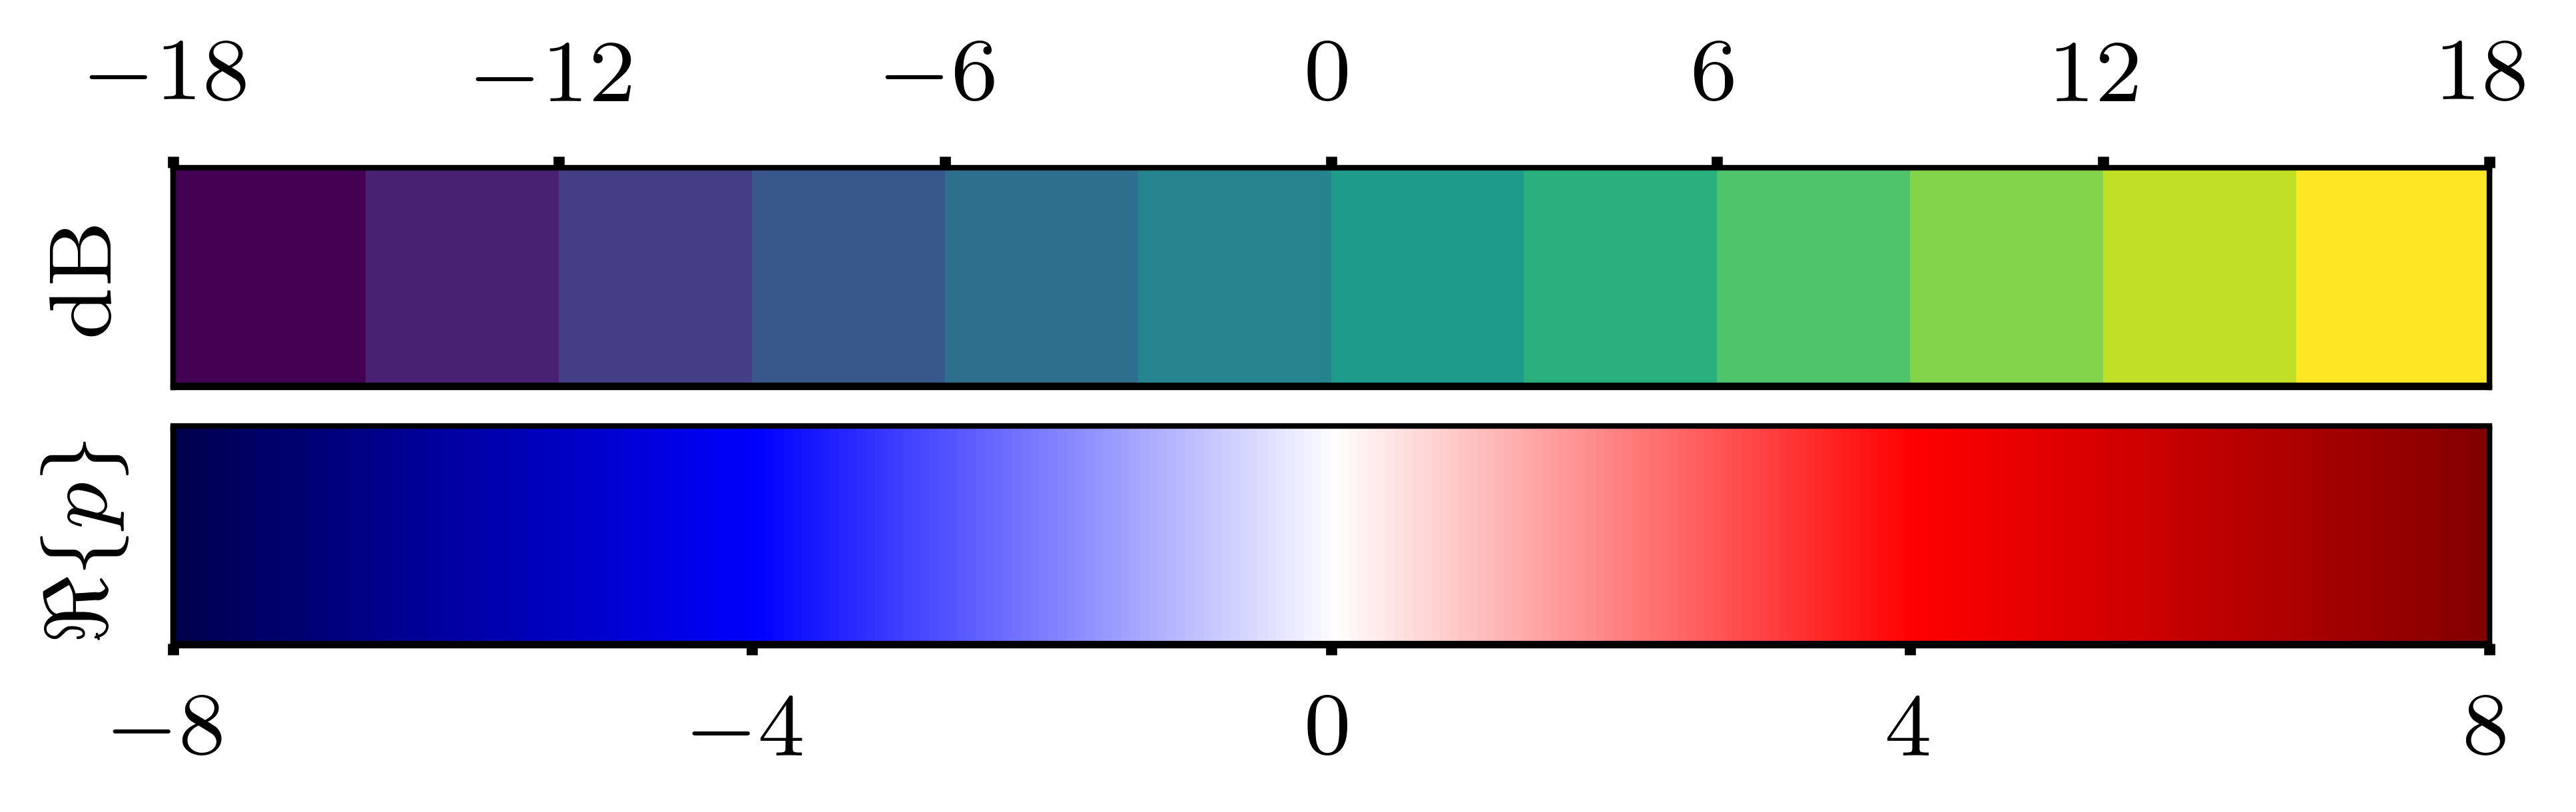
\includegraphics[width=85mm]{../python/plot_colorbar.png}
\end{plotfigures}
\caption{
%Farbskalierung für alle folgenden Grafiken monofrequenter
%Schallfelder.
Colour scales for all subsequent graphics that illustrate single-frequency
sound fields.
%
%Oben: Pegel mit $3$\,dB pro Farbe und $0$\,dB bezogen auf Amplitudenwert Eins.
Top: Sound pressure level with $3$\,dB per colour and $0$\,dB chosen relative
to unit amplitude.
%
%Unten: Realteil der komplexen Schalldruckwechselgröße $p(x_\mathrm{r},y_\mathrm{r})$.
Bottom: Real part of the complex-valued sound pressure $p(x_\mathrm{r},y_\mathrm{r})$.
%
%Schalldruckpegel $>+18\,\text{dB}$ und Schalldruckwerte $>+8$ erfahren eine
%orange Farbsättigung,
Sound pressure level $>+18\,\text{dB}$ and sound pressure $>+8$ is saturated to
orange.
%
%Schalldruckpegel $<-18\,\text{dB}$ und Schalldruckwerte $<-8$ sind mit cyan
%gesättigt.
Sound pressure level $<-18\,\text{dB}$ and sound pressure $<-8$ is saturated to
cyan.
%
\cc
}
\label{fig:plot_colorbar}
\end{figure}



% please DO NOT rescale the figure and keep it single column
\begin{figure}
\centering
\begin{plotfigures}
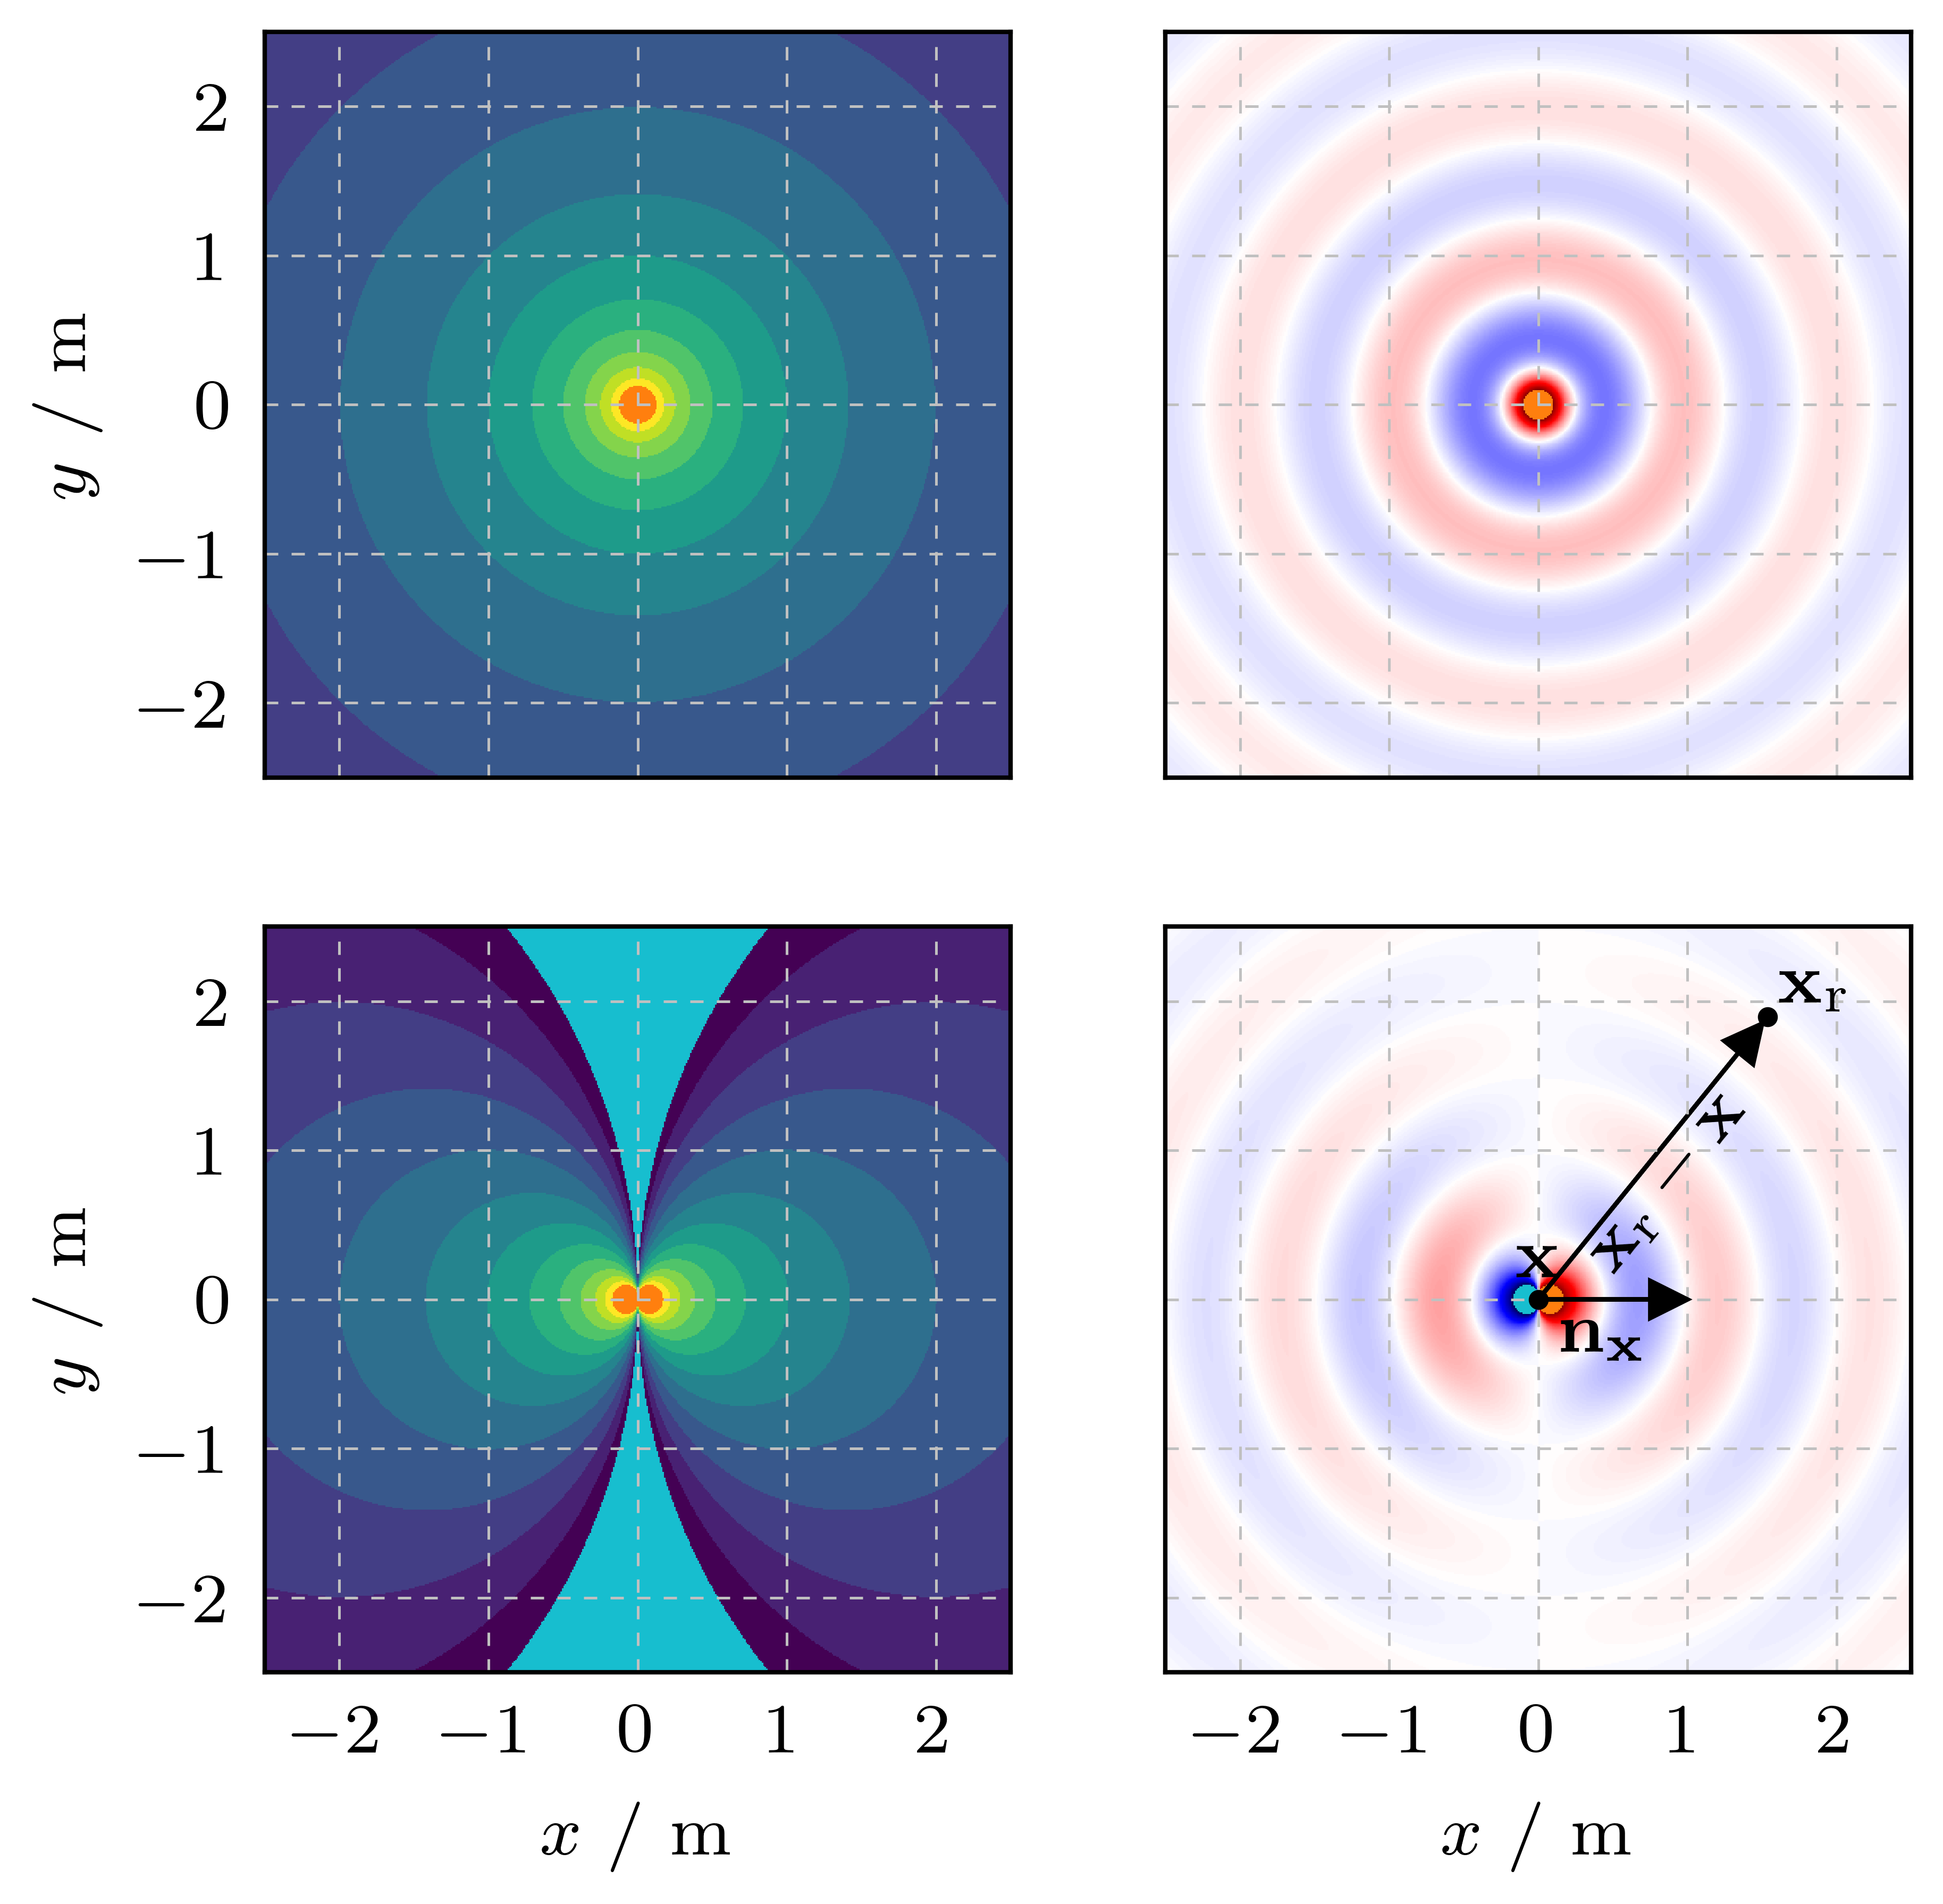
\includegraphics[width=85mm]{../python/monopole_dipole.png}
\end{plotfigures}
\caption{%Schallfeld in der $xy$-Ebene.
Sound field in the $xy$-plane.
%Oben: normalisierter Monopol $4 \pi G(r_{\xs\text{-}\xr})$,
Top: normalised monopole $4 \pi G(r_{\xs\text{-}\xr})$,
%unten: normalisierter Dipol $4 \pi \frac{c}{\omega} G_\text{Dipol}(r_{\xs\text{-}\xr})$.
bottom: normalised dipole $4 \pi \frac{c}{\omega} G_\text{Dipole}(r_{\xs\text{-}\xr})$.
%Quellenposition $\xs=(0,0,0)^\mathrm{T}$\,m,
Source position $\xs=(0,0,0)^\mathrm{T}$\,m,
%Wellenlänge $\lambda=1$ m, Schallgeschwindigkeit $c=343$\,m/s, visualisierter
%Zeitpunkt $t=0$\,s,
wavelength $\lambda=1$\,m, speed of sound $c=343$\,m/s.
%
%Normalen-Richtungsvektor $\nx=(1,0,0)^\mathrm{T}$ zeigt in die Richtung der
%positiven Dipol-Hauptkeule.
The normal vector $\nx=(1,0,0)^\mathrm{T}$ points in the direction of
the positive dipole main lobe at time $t=0$\,s.
%Farbskalierung gemäß \myfig\ref{fig:plot_colorbar}.
Colour scaling according to \myfig\ref{fig:plot_colorbar}.
\cc
}
\label{fig:monopole_dipole}
\end{figure}



%Ein monofrequentes Schallfeld des Monopols ist in
%\myfig\ref{fig:monopole_dipole}~(oben) für die $xy$-Ebene visualisiert.
A single-frequency sound field of the monopole is depicted for the $xy$-plane
in \myfig\ref{fig:monopole_dipole}~(top).
%
%Das omnidirektionale Abstrahlverhalten des Monopols mit $6$\,dB-Pegelabnahme pro
%Entfernungsverdopplung ist ersichtlich.
The omnidirectional radiation characteristic of the monopole, with a loss
of $6$\,dB per doubling of distance is apparent.

%Der Dipol an der Position $\xs$ erzeugt ein monofrequentes Schallfeld, welches
%sich auch aus der \myeq\eqref{eq:G03D} berechnen lässt.
The single-frequency sound field of the dipole at the source position $\xs$ can
be derived from \myeq\eqref{eq:G03D}.
%
%Es ergibt sich aus deren räumlicher Ableitung
%(Gradientenbildung bezüglich $\xs$ mit dem Operator
%$\nabla = (\frac{\partial}{\partial x},\frac{\partial}{\partial y},\frac{\partial}{\partial z})^\mathrm{T}$
%für kartesische Koordinaten)
%und anschließender Projektion (Skalarprodukt) auf den gewünschten
%Normalenvektor $\nx$
It follows from a partial derivation with respect to the spatial coordinates
(i.e. the gradient w.r.t. $\xs$ using the operator
$\nabla = (
\frac{\partial}{\partial x},
\frac{\partial}{\partial y},
\frac{\partial}{\partial z}
)^\mathrm{T}$
in Cartesian coordinates) and a subsequent projection (scalar product) onto
the desired unit normal vector $\nx$
%
\begin{align}
\label{eq:G03D_Dipol}
G_\text{Dipole}(r_{\xs\text{-}\xr}) &=
\nxT \, \nabla G(r_{\xs\text{-}\xr}) \nonumber\\
&= -\nxT\,\bm{\theta}_{\xs\text{-}\xr}\cdot
G(r_{\xs\text{-}\xr}) \cdot \left(\im\wc +\frac{1}{r_{\xs\text{-}\xr}}\right).
\end{align}
%
%Das Skalarprodukt der Vektoren $\bm{n}$ und $\bm{\theta}$ in
%kartesischer Form wird als $\bm{n}^\mathrm{T} \bm{\theta}$ notiert.
% -> not required anymore because already defined above
%
%Der Einheitsvektor
The unit length vector
\begin{align}
\bm{\theta}_{\xs\text{-}\xr} :=
\frac{\xs-\xr}{\|\xs-\xr\|}  =
\frac{\xs-\xr}{r_{\xs\text{-}\xr}}
\end{align}
%zeigt vom Messpunkt $\xr$ zur Dipol- bzw. Monopolposition $\xs$.
shows from the probe point $\xr$ to the dipole or monopole position $\xs$.
%
%Für hohe Frequenzen und/oder weit entfernte Abstände
%$\frac{\omega}{c} r_{\xs\text{-}\xr} \gg 1$ kann Glg.\,\eqref{eq:G03D_Dipol}
%mit
For high frequencies and/or far distances
$\frac{\omega}{c} r_{\xs\text{-}\xr} \gg 1$ holds and the approximation
%
\begin{align}
\label{eq:DipolHF}
G_\text{Dipole}(r_{\xs\text{-}\xr}) \approx
-\nxT\,\bm{\theta}_{\xs\text{-}\xr}\,
G(r_{\xs\text{-}\xr}) \, \im\wc
\end{align}
%
%$G_\text{Dipol}(r_{\xs\text{-}\xr}) \approx
%-\nxT\,\bm{\theta}_{\xs\text{-}\xr}\,
%G(r_{\xs\text{-}\xr}) \, \im\wc$
%genähert werden.
for \eqref{eq:G03D_Dipol} is valid.
%
%In \myfig\ref{fig:monopole_dipole}~(unten) ist beispielhaft das Schallfeld
%eines Dipols visualisiert.
\myfig\ref{fig:monopole_dipole}~(bottom) shows an exemplary sound field
of a dipole.
%
%Der Normalenvektor $\nx$ in Richtung der $x$-Achse zeigt in Richtung der
%zu $t=0$\,s positiven Dipol-Hauptkeule\index{Hauptkeule}.
The normal vector $\nx$ points into the direction of the $x$-axis;
at time $t=0$\,s it also indicates the direction of the positive dipole lobe.
%
%Dies ergibt inhärent die dazu 90$^\circ$ stehende $yz$-Ebene, in welcher der
%Schalldruck beim Dipol Null ist (Dipolnullstelle).
The chosen normal vector inherently determines its orthogonal $yz$-plane,
in which the sound pressure is zero (dipole null).



%Beachtenswert ist die exakte $90^\circ$-Phasenverschiebung zwischen Monopol und
%hochfrequenzgenähertem Dipol.
The exact phase shift of $90^\circ$ between the sound fields of the monopole and
the high-frequency approximated dipole is worth mentioning.



% please DO NOT rescale the figure and keep it single column
\begin{figure}
\centering
\begin{plotfigures}
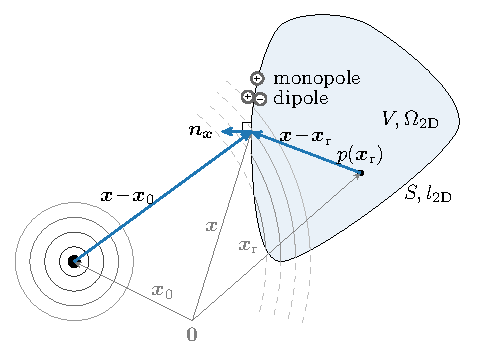
\includegraphics[width=85mm]{../graphics_ENG/khi_geometry.pdf}
\end{plotfigures}
\caption{%Geometrie für das Kirchhoff-Helmholtz-Integral (KHI)
%in \myeq\eqref{eq:KHIGeneral} zur
%Schalldrucksynthese innerhalb eines quellenfreien Volumens $V$.
Geometry for the Kirchhoff-Helmholtz integral equation (KHIE)
in \myeq\eqref{eq:KHIGeneral} for sound pressure synthesis
within a source-free volume $V$.
%
%Positionen $\xs$ von Mono- und Dipolen (Sekundärquellen) auf der Hüllfläche
%$S$ mit herauszeigendem Normalenvektor $\nx$,
Positions $\xs$ for monopoles and dipoles (secondary sources) on the surface $S$
using outward-facing normal vectors $\nx$,
%
%Position $\xp$ der virtuellen Punktquelle (Primärquelle),
position $\xp$ for the virtual source (a.k.a. primary source),
%
%Empfänger-/Mess-/Aufpunkt(e) $\xr$.
receiver positions/probe points $\xr$ within the volume $V$.
%
%In der Praxis wird oft monopolbasierte Schalldrucksynthese mit einer konvexen
%Hüllkontur $l_\text{2D}$ realisiert, welche die Fläche $\Omega_\text{2D}$ in einer
%gewählten Zuhörerebene einschließt.
In practice, sound pressure synthesis based on monopoles
often uses a convex curve $l_\text{2D}$ to enclose the area
$\Omega_\text{2D}$ of a chosen listening plane.
%
Notice the inverted polarity of the dipoles in \myfig\ref{fig:violine}~(right),
which ensures consistency with the negative sign in \eqref{eq:KHIGeneral}.
\cc
}
\label{fig:KHIGeometrie}
\end{figure}



%\subsection{Kirchhoff-Helmholtz-Hüllflächenintegral}
\subsection{Kirchhoff-Helmholtz Integral Equation}

%Nun sei ein Volumen $V$ durch eine Hüllfläche $S$ umschlossen, wie es
%in \myfig\ref{fig:KHIGeometrie} mit dem blauen Körper angedeutet ist.
Now, consider a volume $V$ which is enclosed by the smooth surface $S$, as shown
schematically in \myfig\ref{fig:KHIGeometrie} by the blue shape.
%
%Auf die Hüllfläche werden mit infinitesimalem Abstand
%Monopole und Dipole als sogenannte Sekundärquellen\index{Sekundärquelle}
%platziert.
The surface $S$ is equipped with monopoles and dipoles at infinitesimal
distances, whereby these sources are referred to as secondary
sources\index{secondary source}.
%
%Jedem Punkt $\xs$ auf der Hüllfläche ist ein senkrecht zur Fläche,
%aus dem Volumen herauszeigender Normalenvektor $\nx$ zugewiesen.
Every point $\xs$ on this surface has an outward-facing normal vector $\nx$.
%
%Die exakte und eindeutige Synthese des Schalldrucks $p(\xr)$ wird als
%Schallfeldüberlagerung gewichteter Mono- und Dipole durch das
%als Kirchhoff-Helmholtz-Integral\index{Kirchhoff-Helmholtz-Integral} (KHI)
%bekannte Hüllflächenintegral, vgl. \cite[Kap.~23.2]{Skudrzyk1971}
The precise and unambiguous synthesis of the sound pressure $p(\xr)$ is based
on the superposition of weighted monopole and dipole sound fields, formulated
as Kirchhoff-Helmholtz integral equation (KHIE), cf.~\cite[Ch.~23.2]{Skudrzyk1971}
%
\begin{align} %underbrace sortiert
\label{eq:KHIGeneral}
p(\xr) = \int\limits_S
%\left(
[
&\underbrace{\nxT \, \nabla p(\xs)}_{\text{monopole signal}}\cdot
\underbrace{G(r_{\xs\text{-}\xr})}_{\text{monopole}}
-\nonumber\\
&\underbrace{p(\xs)}_{\text{dipole signal}} \cdot
\underbrace{\nxT \, \nabla G(r_{\xs\text{-}\xr})}_{\text{dipole}}
]
%\right)
\,\mathrm{d}S,
\end{align}
%
%für Empfängerpunkte $\xr$ innerhalb eines quellenfreien Volumens $V$ beschrieben;
for probe points $\xr$ within the source-free volume $V$.
%
%für $\xr$ außerhalb $V$ gilt dann $p(\xr)=0$.
This implies $p(\xr)=0$ for probe points outside the volume.
%
Again, the real part convention
$p(\xr, t) = \Re\{p(\xr) \e^{+\im \omega t}\}$ applies.
%
%Das KHI in \myeq\eqref{eq:KHIGeneral} ist die fundamentale, integrale
%Beschreibung des Phänomens lineare Wellenausbreitung und -überlagerung.
The KHIE in \myeq\eqref{eq:KHIGeneral} represents the fundamental description
of linear wave propagation and superposition in its integral form.
%
%Es ist die Grundlage für Schallfeldsynthese im Allgemeinen, speziell also auch
%für die WFS.
It constitutes the basis of sound field synthesis in general and of WFS
in particular.



%In der Praxis wird das Schallfeld durch die
%Überlagerung von sich ausbreitenden Schallfeldern der individuell angesteuerten
%Lautsprecher erzeugt, und somit $p(\xr)$ über eine diskrete Summation erzeugt.
For practical reasons, the integral is approximated by a discrete, finite sum,
since the sound field $p(\xr)$ is generated by the superposition of propagating
sound fields from a finite number of individually controlled loudspeakers.
%
%Die resultierende, physikalisch begründete Approximation des eigentlich
%intendierten Schallfeldes ist charakteristisch für alle KHI-basierten
%Schallfeldsyntheseverfahren, daher nicht WFS-spezifisch.
%
This physically motivated approximation of the intended sound field is
a feature of all sound field synthesis methods derived from KHIE, and
is therefore not specific to the WFS.
%
%Der Schalldruckverlauf über die Zeit wird mit $\Re\{p(\xr)\cdot\e^{+\im \omega t}\}$
%für ein monofrequentes Schallfeld mit der Kreisfrequenz $\omega$
%berechnet.
%For a chosen $\xr$, the real part convention $\Re\{p(\xr)\cdot\e^{+\im \omega t}\}$
%yields a sound pressure function over time for a single-frequency sound field with
%a specific angular frequency $\omega$. -> phrase moved up and considerably shortened



%\subsection{Gewichtungssignale für daten- und modellbasierten WFS-Ansatz}
\subsection{Driving Signals for Data-Based and Model-Based WFS}

%Mit der WFS können Schallszenarien, oft auch akustische
%Szenen genannt, bestehend aus räumlich und zeitlich gestaffelten Wellenfronten
%synthetisiert werden.
With the WFS, desired sound scenarios, often referred to as acoustic scenes,
are synthesised by the spatio-temporal superposition of wavefronts.
%
%Im WFS-Kontext gibt es zwei grundständige Herangehensweisen zur Erzeugung von
%akustischen Szenen: die datenbasierte und die modellbasierte.
In the context of the WFS, two pivotal approaches exist: the data-based and the
model-based one.
%
%Die datenbasierte WFS, vgl. \cite{Berkhout1988_JAES}
%verarbeitet direkt akustische Messungen als WFS-Ansteuerungssignale,
%wie in \myfig\ref{fig:violine} angedeutet.
For the data-based WFS, cf.~\cite{Berkhout1988_JAES}, the loudspeaker driving
signals are directly processed from acoustic measurements/recordings,
as shown in \myfig\ref{fig:violine}.
%
%Die modellbasierte WFS, vgl. \cite{Berkhout1993_JASA}
%arbeitet mit Modellen für virtuelle Schallquellen wie in
%\myfig\ref{fig:KHIGeometrie} skizziert.
The model-based WFS, cf.~\cite{Berkhout1993_JASA}, exploits models
for virtual sound sources, as sketched in \myfig\ref{fig:KHIGeometrie}.
%
%Dieser Ansatz ist Bestandteil von objektbasierter Wiedergabe
%\cite{Vaananen2002, Plogsties2003, Plogsties2003, Brandenburg2004, Geier2008,
%Spors2013_IEEE,Sporer2018_book},
%für die Audiosignal, Modelltyp und -parametrik einem, mit der WFS zu
%spatialisierenden, Audio-Objekt zugewiesen werden.
This model-based strategy is part of object-based reproduction
\cite{Vaananen2002, Plogsties2003,Plogsties2003, Brandenburg2004,
Geier2008,Spors2013_IEEE,Sporer2018_book},
in which the audio signal, the model type and its parameters are assigned
to an audio object to be spatialised.



%Die Gewichtungssignale $\nxT \, \nabla p(\xs)$ für die Monopole im KHI
%(in \myeq\eqref{eq:KHIGeneral} als Monopolsignal bezeichnet)
%sind die normalen-projizierten Schalldruckgradienten auf der Hüllfläche.
The driving signals $\nxT \, \nabla p(\xs)$ for the monopoles in the
KHIE -- referred to as monopole signal in \myeq\eqref{eq:KHIGeneral} -- originate
from the directional derivative with respect to the outward-facing normal.
%
%Diese Signale sind proportional zur normalen Schallschnelle bezüglich der Hüllfläche,
%vgl. \cite{Berkhout1993_JASA, Vries1996_JAES}.
These signals are related to the normal component of the surface's particle
velocity, cf. \cite{Berkhout1993_JASA, Vries1996_JAES}.
% cf. \cite[Ch.~24.8]{Skudrzyk1971}: `particle velocity in the plane of the screen,
% or velocity of piston membrane'
% cf. E.G. Williams, Fourier Acoustics, p.33ff
%
%Beim datenbasierten Direkt-Wiedergabeansatz stammen sie von
%Messungen bzw. von Aufnahmen mit Druckgradientenmikrofonen
%mit Achter-Richtcharakteristik, wobei die Hauptkeule
%orthogonal zur Hüllfläche ausgerichtet ist, vgl.~\myfig\ref{fig:violine}.
For the data-based approach, recordings made with pressure-gradient,
figure-of-eight microphones can be reproduced directly, assuming that
the reproduction surface and the recording surface exhibit identical shape.
Further, to do so, the normal direction of the
figure-of-eight microphones/dipole loudspeakers must be orthogonally aligned
to the recording/reproduction surface, cf.~\myfig\ref{fig:violine}.



%Die Gewichtungssignale $p(\xs)$ für die Dipole im KHI (in
%\myeq\eqref{eq:KHIGeneral} als Dipolsignal bezeichnet)
%entsprechen den Schalldrücken auf der Hüllfläche.
The driving signals $p(\xs)$ for the dipoles in the KHIE -- referred to as dipole
signals in \myeq\eqref{eq:KHIGeneral} -- are directly proportional to the
sound pressure on the surface.
%
%Diese können für den datenbasierten Ansatz direkt mit omnidirektionalen
%Druckempfängern aufgezeichnet werden.
For the data-based approach, these signals can be directly recorded with
omnidirectional pressure microphones.



%Die datenbasierte Direktwiedergabe entspricht im Wesen der Utopie
%von \cite{Fletcher1934,Steinberg1934} ohne weitere
%Signalaufbereitung zwischen \textit{screen of microphones} und
%\textit{screen of loudspeakers} \cite[S.\,572]{Snow1953}.
Data-based direct reproduction corresponds to the essence of the 1930s'
technical utopia  \cite{Fletcher1934,Steinberg1934}, not considering signal
processing in between
the `screen of microphones' and
the `screen of loudspeakers' \cite[p.~572]{Snow1953}.
%
%Die Manipulationsmöglichkeiten räumlicher und zeitlicher Parameter beim
%datenbasierten Ansatz mit Zwischenverarbeitung der Mikrofonsignale sind
%eingeschränkt, dafür kann die räumlich-zeitliche Komplexität eines
%Schallfeldes durch geeignete Messauflösung vergleichsweise
%einfach erfasst und synthetisiert
%werden, vgl. \cite{Sonke2000_diss,Hulsebos2004_diss,Vries2007_JASP}.
The spatio-temporal complexity of a sound field can be captured comparably
simply with appropriate measurement resolution, but the possibilities
for spatio-temporal manipulation of such recorded data is limited for
WFS purposes, cf. \cite{Sonke2000_diss,Hulsebos2004_diss,Vries2007_JASP}



%Beim modellbasierten Ansatz errechnen sich die benötigten Gewichtungssignale
%$\nxT \, \nabla p(\xs)$ und $p(\xs)$ aus dem Schallfeld eines analytisch
%gegebenen Quellenmodells -- z.B. eine außerhalb von $V$ befindliche Punktquelle,
%wie jene bei $\xp$ in \myfig\ref{fig:KHIGeometrie} -- dem ein zu spatialisierendes
%Audiosignal aufgeprägt wird.
In contrast, the model-based strategy is employed to spatialise audio objects.
The required driving signals $\nxT \, \nabla p(\xs)$ and $p(\xs)$ need to be
calculated from analytically given source models, for example, for a point source
at $\xp$ outside the volume $V$ as shown in \myfig\ref{fig:KHIGeometrie}.
%
%Ein Quellenmodell wird im WFS-Kontext oft als virtuelle Quelle oder als
%Primärquelle\index{Primärquelle} bezeichnet.
In the WFS terminology, a source model is often referred to as a virtual source
or primary source\index{primary source}.
%
%Die auf der Hüllfläche $S$ positionierten Mono- und Dipole werden hingegen
%als Sekundärquellen\index{Sekundärquelle} bezeichnet.
The monopoles and the dipoles on the surface $S$, utilised for the synthesis,
are termed secondary sources.
%
%Beim modellbasierten Wiedergabeansatz
%werden typischerweise einfache Quellenmodelle gewählt, einhergehend mit vergleichsweise
%geringer Schallfeldkomplexität, dafür aber mit einfacher Variationsmöglichkeit
%der Raum-Zeit-Parametrik des Quellenmodells.
For the model-based reproduction approach, simple source models are typically
chosen, accompanied by comparatively low sound field complexity, but with the
advantage of straightforward and convenient variation of the spatio-temporal
parameters of the source model.
%
%Einfache virtuelle Quellenmodelle sind die
%Punktquelle \cite{Berkhout1993_JASA,Start1997_diss},
%die sogenannte fokussierte Punktquelle \cite{Verheijen1997_diss,Spors2007b,
%Melchior2008,Wierstorf2014_diss}
%und die ebene Welle \cite{Spors2008a, Voelk2012, Firtha2019_diss}.
Simple virtual source models are
the point source \cite{Berkhout1993_JASA,Start1997_diss},
the so called focused point source \cite{Verheijen1997_diss,Spors2007b,
Melchior2008,Wierstorf2014_diss} and
the plane wave \cite{Spors2008a, Voelk2012, Firtha2019_diss}.
%
%Das ebene Wellenmodell kann als Grenzfall der sehr weit
%entfernten Punktquelle aufgefasst werden.
The virtual plane wave model can be regarded as a limiting case of a very
distant virtual point source.
%
%Für die Punktquelle wurden Modellerweiterungen für Quellrichtcharakteristika und
%Bewegungstrajektorien diskutiert, vgl. \cite{Corteel2007_JASP,Baalman2008_diss,Franck2012,
%Romoli2015_ApplAc,Schultz2017,Franck2007,Ahrens2011,Firtha2019_diss}.
For the virtual point source, model extensions for far-field directivities and
for motion trajectories were discussed, cf. \cite{Corteel2007_JASP,Baalman2008_diss,
Franck2012,Romoli2015_ApplAc,Schultz2017,Franck2007,Ahrens2011,Firtha2019_diss}.



%Beiden Ansätzen, dem daten- bzw. dem modellbasierten, ist ein gemessener bzw.
%ein gewünschter, analytisch bekannter Wellenfrontverlauf gemein, der auf Basis
%des KHIs rekonstruiert bzw. synthetisiert werden soll.
Both approaches, the data-based and the model-based, have in common that
either a measured wavefront or a desired, analytically accessible wave field
is to be either reconstructed or synthesised based on the KHIE.
%
%Daraus resultieren die in der Literatur synonym verwendeten Begriffe
%Wellenfrontsynthese\index{Wellenfrontsynthese} und
%Wellenfeldsynthese \cite{Berkhout1992b,Berkhout1992a}.
This motivates the terms `wavefront synthesis'\index{wavefront synthesis} and
`wave field synthesis'\index{wave field synthesis}, which are used synonymously
in the literature, cf. \cite{Berkhout1992b,Berkhout1992a}.



%\section{Modellbasierter Ansatz für die WFS einer virtuellen Punktquelle}
\section{Model-Based Approach for WFS of a Virtual Point Source}
\label{sec:WFS_PointSource}

%Weil die virtuelle Punktquelle ein fundamentales Quellenmodell darstellt und in
%der WFS-Produktionspraxis eine wichtige Rolle spielt, soll im Folgenden
%auf die modellbasierte WFS der virtuellen Punktquelle näher eingegangen werden.
Since the point source is a fundamental virtual source model and plays an
important role in WFS production practice, this section takes a closer look at
the model-based WFS of the virtual point source.
%
%Diese soll bei $\xp$ außerhalb von $V$ positioniert sein\footnote{Die sogenannte
%fokussierte Quelle erhält man, wenn $\xp$ innerhalb von $V$ zugelassen wird,
%was hier zu Gunsten anderer Inhalte nicht im Detail diskutiert wird.},
%vgl.~\myfig\ref{fig:KHIGeometrie}.
This source should be positioned outside of the volume\footnote{The so called
focused point source allows source positions within the volume. This is not
discussed here in favour of other details.} at $\xp$ as sketched in
\myfig\ref{fig:KHIGeometrie}.
%
%Damit definiert sich der Einheitsvektor
The resulting unit length vector
\begin{align}
\bm{\theta}_{\xs\text{-}\xp} :=
\frac{\xs-\xp}{\|\xs-\xp\|} =
\frac{\xs-\xp}{r_{\xs\text{-}\xp}}
\end{align}
%von der virtuellen Punktquelle $\xp$ zu einem Hüllflächenpunkt
%$\xs$ zeigend.
points from the virtual source position $\xp$ towards a position $\xs$ on the
secondary source surface.
%
%Der Abstand zwischen diesen beiden Punkten ist
%$r_{\xs\text{-}\xp}=\|\xs-\xp\|$.
The distance between these two points is $r_{\xs\text{-}\xp}=\|\xs-\xp\|$.



%\subsection{Fernfeld-/Hochfrequenz-Näherung des KHI}
\subsection{Far-Field/High-Frequency Approximation of the KHIE}

%Die virtuelle Punktquelle mit komplexer Amplitude $A$ erzeugt auf der Hüllfläche $S$
%das monofrequente Schallfeld
The virtual point source shall exhibit a complex-valued amplitude $A$.
Then the single-frequency sound field $p(\xs) = A \cdot G(r_{\xs\text{-}\xp})$
holds on the surface $S(\xs)$.
%
%Für die Synthese einer Wellenfront ausgehend von dieser virtuellen Punktquelle
%wird $p(\xs)$ in das KHI in \myeq\eqref{eq:KHIGeneral} eingesetzt.
For the synthesis of the wavefront emanating from the virtual point source,
this sound pressure $p(\xs)$ is inserted into the KHIE
\myeq\eqref{eq:KHIGeneral}.
%
%Unter den Bedingungen
%$\wc r_{\xs\text{-}\xr} \gg 1$ und
%$\wc r_{\xs\text{-}\xp} \gg 1$
%kann der Integrand genähert werden (vgl.~\myeq\eqref{eq:G03D_Dipol} und
%\eqref{eq:DipolHF}), was zum Schallfeld $p(\xr)$
Under the conditions
$\wc r_{\xs\text{-}\xr} \gg 1$ and
$\wc r_{\xs\text{-}\xp} \gg 1$
the integrand can be approximated (cf.~\myeq\eqref{eq:G03D_Dipol} and
\eqref{eq:DipolHF}), which yields the sound field
%
\begin{align}
%\label{eq:KHIFarMono}
p(\xr) \approx \int\limits_S [
&\underbrace{-A\,
\im\wc\,
\nxT \bm{\theta}_{\xs\text{-}\xp}\,
G(r_{\xs\text{-}\xp})}_{\text{monopole signal, Far/HF approximated}}
%
\cdot \underbrace{G(r_{\xs\text{-}\xr})}_{\text{monopole}}-
\nonumber\\
&\underbrace{A \, G(r_{\xs\text{-}\xp})}_{\text{dipole signal}}
\cdot
\underbrace{(-\im\wc)\,
\nxT \bm{\theta}_{\xs\text{-}\xr}\,
G(r_{\xs\text{-}\xr})}_{\text{dipole, Far/HF approximated, cf.~\eqref{eq:DipolHF}}}
%
]\,\mathrm{d}S.
\end{align}
%
%führt und die Grundlage zur Beschreibung
%der in Seismik, Optik und Akustik bekannten Fresnel-Kirchhoff-Beugung einer
%Punktquelle darstellt, sowie Ausgangspunkt der
%High Frequency Boundary Element Method
%(HF-BEM) ist, vgl. \cite{Schultz2016_diss, Zotter2013, Firtha2019_diss}.
This equation is used to describe Fresnel–Kirchhoff diffraction from
a point source, a phenomenon that is well understood in the fields of
seismology, optics, and acoustics.
It is further the starting point for the high-frequency boundary
element method (HF-BEM),
cf. \cite{Schultz2016_diss, Zotter2013, Firtha2019_diss}.
%
%Diese auch für WFS verwendeten Fernfeld- und/oder
%Hochfrequenznäherungen
%\index{Fernfeld-/Hochfrequenznäherung}
%\index{Hochfrequenz-/Fernfeldnäherung}
%fordern, dass die jeweiligen Abstände
This far-field and/or high-frequency approximation
\index{far-field/high-frequency approximation}
\index{high-frequency/far-field approximation}
is also used in the WFS
and requires the respective distances
%\begin{align}
%r_{\xs\text{-}\xp}=\|\xs-\xp\|\qquad
%r_{\xs\text{-}\xr}=\|\xs-\xr\|
%\end{align}
%$r_{\xs\text{-}\xp}=\|\xs-\xp\|$ (virtuelle Quelle zu Sekundärquelle) und
%$r_{\xs\text{-}\xr}=\|\xs-\xr\|$ (Sekundärquelle zu Empfänger)
$r_{\xs\text{-}\xp}=\|\xs-\xp\|$ (virtual source to secondary source) and
$r_{\xs\text{-}\xr}=\|\xs-\xr\|$ (secondary source to receiver point)
%
%deutlich größer sind als die betrachtete Wellenlänge
to be significantly larger than the considered wavelength
$\lambda = 2\pi\frac{c}{\omega}$.
%
%Das Integral kann umgeschrieben werden zu
The integral can be rewritten as
%
%\begin{align}
%\label{eq:KHIFarMono}
%p(\xr) \approx \int\limits_S A \cdot
%&\underbrace{\im\wc \cdot \nxT\left(\bm{\theta}_{\xs\text{-}\xr} - \bm{\theta}_{\xs\text{-}\xp}\right)
%\cdot G(r_{\xs\text{-}\xp})}_{\substack{\text{Grundlage für Ansteuerung } D(\xp,\xs) \text{,} \\ \text{Dipol Abhängigkeit}}}
%\times\nonumber\\
%&\underbrace{G(r_{\xs\text{-}\xr})}_{\text{Monopol}}
%\mathrm{d}S,
%\end{align}
\begin{align}
\label{eq:KHIFarMono}
p(\xr) \approx \int\limits_S A \cdot
&\underbrace{\im\wc \cdot \nxT\left(\bm{\theta}_{\xs\text{-}\xr} - \bm{\theta}_{\xs\text{-}\xp}\right)
\cdot G(r_{\xs\text{-}\xp})}_{\substack{\text{fundament for loudspeaker signal } D(\xp,\xs) \text{,} \\ \text{dipole dependence!}}}
\times\nonumber\\
&\underbrace{G(r_{\xs\text{-}\xr})}_{\text{monopole}}
\mathrm{d}S.
\end{align}
%wobei beachtenswert ist, dass trotz der Freistellung des
%Monopolquelltyps in \myeq\eqref{eq:KHIFarMono} hochfrequenzgenäherte
%Sekundär-Dipole mit dem Term $\im\wc\,\nxT\,\bm{\theta}_{\xs\text{-}\xr}\,
%G(r_{\xs\text{-}\xr})$ enthalten sind, vgl.~\eqref{eq:DipolHF}.
It is important to note that the monopole is weighted by a term containing
a secondary dipole source\index{secondary dipole source} dependence,
cf. the expression $\im\wc\,\nxT\,\bm{\theta}_{\xs\text{-}\xr}\,
G(r_{\xs\text{-}\xr})$ found in the first term of \eqref{eq:KHIFarMono}
with the expression in \eqref{eq:DipolHF}.



%\subsection{Monopolbasierte 3D- und 2.5D-Syntheseintegrale}
\subsection{Monopole-Based 3D and 2.5D Synthesis Integrals}

%Um den praktischen Aufwand maßvoll zu gestalten, wird bei der Realisierung von WFS
%typischerweise nur ein Lautsprechertyp für die Sekundärquellen verwendet,
%vgl. \cite{Vries1996_JAES}.
In practice, only one loudspeaker type is usually employed as a secondary
source, aiming at moderate technical effort, cf. \cite{Vries1996_JAES}.
%
%Diese Einschränkung für das KHI hat zur Folge,
%dass auch ein Schallfeld außerhalb des Synthesevolumens
%erzeugt wird, welches einen etwaigen Wiedergaberaum anregt,
%vgl. \cite{Start1997_diss, Wittek2007_JAES, Wittek2007_diss, Gauthier2007_Acta,Erbes2020_diss},
%und das gewünschte Schallfeld von Raumreflexionen überlagert wird.
%
This restriction for the KHIE implies a sound field outside the synthesis volume,
which stimulates a potential venue, cf. \cite{Start1997_diss, Wittek2007_JAES,
Wittek2007_diss, Gauthier2007_Acta,Erbes2020_diss}.
Room reflections are then superimposed on the intended sound field.
%
%Typische Lautsprecherboxen verhalten sich im tieffrequenten, für WFS praktikablen
%Frequenzbereich (vgl.~\myeq\eqref{eq:SamplingCriterion})
%annähernd monopolartig und weisen mit zunehmender Frequenz
%eine zunehmende Richtwirkung zur Frontalrichtung hin auf.
Typical loudspeakers behave like a monopole in the WFS-relevant,
low-frequency range (cf.~\myeq\eqref{eq:SamplingCriterion}) and exhibit
increasing directivity towards the frontal direction as the frequency rises.
%
%Die weitere Betrachtung erfolgt daher vereinfachend mit Monopolen und
%ohne Berücksichtigung von Raumeinflüssen, d.h. für Freifeldbedingungen.
For the sake of simplicity, the subsequent analysis is therefore carried
out using secondary monopole sources\index{secondary monopole source}.
Room reflections are not taken into account, i.e. free-field conditions
are assumed.



%Das Integral für 3D-Synthese\index{3D-Synthese} mit Monopolen auf der Hüllfläche $S$
%kann allgemeiner
The integral for 3D synthesis\index{3D synthesis} using monopoles on the
surface $S$ can be written more generally as
\begin{align}
p(\xr) =&
\int\limits_S A \, D_\text{3D}(\xp,\xs) \, G(r_{\xs\text{-}\xr}) \, \mathrm{d}S.
\label{eq:MonopolIntegral_3D}
\end{align}
%geschrieben werden.
%Die unbekannte, sogenannte Treiberfunktion $D_\text{3D}(\xp,\xs)$
%stellt eine lautsprecherindividuelle, komplexe Gewichtung der
%Eingangssignalamplitude $A$ der virtuellen Punktquelle dar.
For each loudspeaker, the unknown, so called driving function
$D_\text{3D}(\xp,\xs)$ represents a complex-valued weighting of the input signal
amplitude $A$.
%
%Das komplexe Gewicht geht bei breitbandiger Betrachtung in das Spektrum
%$D_\text{3D}(\xp,\xs,\omega)$ über.
When considering broadband signals, the driving signal represents a
filter impulse response $d_\text{3D}(\xp,\xs, t)$.
%
Its corresponding frequency response is denoted as $D_\text{3D}(\xp,\xs,\omega)$.
%
% we don't need this in the ENG version:
%Dieses wird im Folgenden Filter-Frequenzgang genannt, um es eindeutig
%vom Frequenzgang eines breitbandigen Schallfeldes, welcher an einem
%bestimmten Empfängerpunkt gemessen wird, unterscheidbar zu machen.
%
As there is no ambiguity, both
the weight $D_\text{3D}(\xp,\xs)$ and
the spectrum $D_\text{3D}(\xp,\xs,\omega)$
are referred to as driving functions
in the following.
%
%Breitbandig ergibt sich im Frequenzbereich somit die Multiplikation des
%Audio-Eingangssignalspektrums $A(\omega)$ der virtuellen Quelle
%mit dem lautsprecherindividuellen Filter-Frequenzgang
%$D_\text{3D}(\xp,\xs,\omega)$ der gesuchten WFS-Ansteuerung.
Thus, for broadband signals, the input signal spectrum $A(\omega)$
is multiplied by the yet unknown driving function
$D_\text{3D}(\xp,\xs,\omega)$.



%Um den praktischen Aufwand weiter zu reduzieren, wird statt
%einer Hüllfläche $S$ eine Hüllkontur $l_\text{2D}$ verwendet.
To further reduce the practical effort, a curve $l_\text{2D}$
equipped with loudspeakers is used instead of a surface $S$.
%
%Für die WFS innerhalb einer Horizontalebene kommen dabei oft lineare bzw.
%kreis- oder rechteckartig umhüllende Lautsprecherarrays zum Einsatz,
%idealerweise auf Ohrhöhe,
%vgl.~\myfig\ref{fig:WFS_Array_Haus8}, \cite{Vries2009_Mono,Vries2019}.
For WFS in a horizontal plane, linear arrays or enclosing rectangular or circular
arrays are typically used, ideally positioned at the listener's ear level,
cf.~\myfig\ref{fig:WFS_Array_Haus8} and \cite{Vries2009_Mono,Vries2019}.
%
%Das Syntheseintegral mit Monopolen auf der Hüllkontur $l_\text{2D}$
%lautet allgemein
The monopole-based synthesis integral for a curve $l_\text{2D}$
generally reads
\begin{align}
p(\xr) =&
\int\limits_{l_\text{2D}} A \, D_\text{2.5D}(\xp,\xs,\xr) \, G(r_{\xs\text{-}\xr}) \, \mathrm{d}l_\text{2D}.
\label{eq:MonopolIntegral_25D}
\end{align}
%
%Für diesen Fall wird typisch und praxisrelevant angenommen, dass
%virtuelle Quelle, Hüllkontur und Empfängerpunkte in der gleichen Ebene liegen.
For practical reasons, it is assumed that the virtual source $\xp$,
the secondary source curve $l_\text{2D}(\xs)$
and the listener positions $\xr$ are all in the same plane.



%Das Linienintegral und die betrachtete Syntheseebene sind zwei-dimensional,
%der gewählte Primär- und Sekundärquellentyp Monopol erzeugt hingegen ein
%drei-dimensionales Schallfeld.
The line integral and the considered synthesis plane are both two-dimensional (2D),
whereas the chosen primary and secondary source type, the monopole, creates
a 3D sound field.
%
%Die Synthese mit \myeq\eqref{eq:MonopolIntegral_25D} liefert nun daher
%zwar ein 3D-Schallfeld, welches aber nur von zwei ortsspezifischen
%Variablen abhängig ist und
%entsprechend nur in 2D kontrolliert bzw. parametrisiert werden kann.
The synthesis with \myeq\eqref{eq:MonopolIntegral_25D} results in a
3D sound field that depends only on two specific spatial variables
and can therefore only be controlled and parametrised in 2D.
%
%Dies ist in der Wellentheorie bekannt als zweieinhalb-dimensionales
%Problem \cite{Bleistein1986}. %,Bleistein2001}.
In wave theory, this is well known as a two-and-a-half-dimensional
(2.5D) problem \cite{Bleistein1986}.
%
%Die zugeschnittene, gesuchte Treiberfunktion $D_\text{2.5D}(\xp,\xs,\xr)$ bzw.
%der Filter-Frequenzgang $D_\text{2.5D}(\xp,\xs,\xr,\omega)$ erhalten daher
%den Index \text{2.5D}, um die zweieinhalb-dimensionale WFS, also
%die 2.5D-Synthese\index{2.5D-Synthese}, klar vom 3D-WFS-Fall abzugrenzen.
The customised unknown driving functions
$D_\text{2.5D}(\xp,\xs,\xr)$ and $D_\text{2.5D}(\xp,\xs,\xr,\omega)$,
respectively are denoted with the index 2.5D, to distinguish
the 2.5D WFS scenario (2.5D synthesis\index{2.5D synthesis}) from
the 3D WFS scenario (3D synthesis\index{3D synthesis}).



%Die Integrale in den \myeqn\eqref{eq:MonopolIntegral_3D}, \eqref{eq:MonopolIntegral_25D}
%stellen Faltungen bezüglich der Ortsvariablen dar.
The integrals in
\myeqn\eqref{eq:MonopolIntegral_3D}, \eqref{eq:MonopolIntegral_25D}
represent convolutions with respect to the spatial variables.
%
%Sie sind selten geschlossen analytisch berechenbar.
They are very rarely analytically solvable.
%
%Die gesuchte Treiberfunktion / der Filter-Frequenzgang $D_{\cdot\text{D}}$
%ist Teil des Integranden.
The unknown driving function $D_{\cdot\text{D}}$ is part of the integrand.
%
%Drei wesentliche Verfahren zum Lösen nach der Treiberfunktion sind möglich:
There are three known fundamental methods of solving for the driving
function:
%
%a) numerische Lösungen aus einem diskretisierten, inversen
%Problem, vgl.
a) numerical solutions originating from a discretised inverse problem, cf.
\cite{Ise1999,Kolundzija2009a,Bai2015_JASA,Koyama2020_IEEE},
%b) explizite analytische Lösungen für einfache Geometrien als räumliches
%Entfaltungsproblem
b) explicit analytical solutions for simple geometries originating from
spatial deconvolution \cite{Ahrens2008_Acta,Spors2010a,Ahrens2010_IEEE,
Fazi2010,Koyama2013},
%und c) die implizite analytische Lösung, bei dem die Ansteuerungsfilter
%aus dem Integranden der Hochfrequenznäherung in \myeq\eqref{eq:KHIFarMono}
%extrahiert werden können.
and c) the implicit analytical solution, which extracts the driving function
from the integrand of the far-field/high-frequency approximated expression
in \myeq\eqref{eq:KHIFarMono}.



%Für Audioanwendungen wurde letztgenannte Methode als WFS in
%\cite{Berkhout1993_JASA, Vries1996_JAES}
%für die planare bzw. die lineare Sekundärquellengeometrie
%unter Benutzung der sogenannten Rayleigh-Integrale \cite[Kap.~25.5]{Skudrzyk1971}
%eingeführt und in Folge in
%\cite{Start1997_diss,Verheijen1997_diss,Voelk2012,Zotter2013,Firtha2019_diss,
%ZotterSchultz2020_White}
%konsolidierend ausformuliert.
The latter method was introduced for audio applications as the WFS for planar
and linear secondary source geometries, utilising the Rayleigh integrals
\cite[Ch.~25.5]{Skudrzyk1971}, and was subsequently formulated in
a consolidated manner by \cite{Start1997_diss,Verheijen1997_diss,Voelk2012,
Zotter2013,Firtha2019_diss,ZotterSchultz2020_White}.



%Die theoretische Abhandlung \cite{Firtha2019_diss} für die WFS von
%allgemeinen konvexen, divergierenden Wellenfronten inklusive physikalisch korrekter
%Abbildung bewegter Quellen liefert eine stringente Analyse lokaler
%Wellenfrontkrümmungen und Wellenrichtungsvektoren für verschiedene
%Schallfeldsyntheseintegrale.
The theoretical work \cite{Firtha2019_diss} presents a rigorous analysis of
local wavefront curvatures and local wave number vectors for various
sound field synthesis integrals.
This has enabled a discussion of general convex and divergent wavefronts,
as well as an analytical description for the physically correct synthesis of
moving sound sources.
%
%Mit dieser Sichtweise können die bekannten WFS-Lösungen konsistent verortet und
%z.B. für bewegte Quellen \cite{Franck2007, Ahrens2011} erweitert werden.
Using this WFS framework, \cite{Firtha2019_diss} classified the published
WFS solutions and enhanced them for moving sources,
that were initially introduced in \cite{Franck2007, Ahrens2011}.
%
%Basierend auf \cite{ZotterSchultz2020_White} soll
%eine diesem Kapitel angemessen kompakte, verallgemeinernde Betrachtung
%weiterverfolgt werden.
Based on \cite{ZotterSchultz2020_White}, a sufficiently concise and
generalised consideration will be pursued in this chapter.



%\subsection{WFS als implizite Lösung mit Sattelpunktsnäherung}
\subsection{WFS as an Implicit Solution from the Stationary Phase
Approximation}

%Für die implizite Lösung nach der Treiberfunktion muss das Integral
%in \myeq\eqref{eq:KHIFarMono} weiter vereinfacht werden.
Further simplifications of the integrand in \myeq\eqref{eq:KHIFarMono}
are required to obtain the implicit solution.
%
%Vor allem muss für die intendierte monopolbasierte Synthese
%der in \myeq\eqref{eq:KHIFarMono} noch vorhandene Sekundärquellentyp Dipol
%eliminiert werden.
Above all, the dependence on the secondary dipole source type
% in \myeq\eqref{eq:KHIFarMono}
must be eliminated for the intended monopole synthesis.
%
%Die Vereinfachung gelingt mit der sogenannten Sattelpunktsnäherung
%\index{Sattelpunktsnäherung}
%(\textit{stationary phase approximation}), welche
%die Hochfrequenznäherung voraussetzt.
This can be achieved using the so called stationary phase approximation
(SPA)\index{stationary phase approximation} \cite[Ch.~3.1]{Start1997_diss},
\cite[Ch.~3.3]{Firtha2019_diss} which assumes that the
far-field and/or high-frequency approximations are met.
%
%Die Sattelpunktsnäherung liefert den Schalldruck für \textit{einen} beliebigen
%Empfängerpunkt $\xr$ im Zuhörerbereich für 3D-Synthese
Then, the SPA yields the sound pressure for \textit{one} arbitrary
probe point $\xr$ in the listening area for the 3D synthesis
%
\begin{align}
\label{eq:pStat3D}
p(\xr) \approx A \cdot G(r_{\xr\text{-}\xp})
\end{align}
%
%und für 2.5D-Synthese
and for the 2.5D synthesis
%
\begin{align}
\label{eq:pStat25D}
p(\xr) \approx A\cdot
\sqrt{\frac{\frac{\im \omega}{c}}{2\pi}}\sqrt{\frac{r_{\xs\text{-}\xr} + r_{\xs\text{-}\xp}}{r_{\xs\text{-}\xr} \cdot r_{\xs\text{-}\xp}}}\cdot G(r_{\xr\text{-}\xp}),
\end{align}
respectively.
%
%Das komplexe Gewicht $G(r_{\xr\text{-}\xp})$ beschreibt die Schallausbreitung
%einer Punktquelle
%bei $\xp$ zum Empfängerpunkt $\xr$ mit dem Abstand $r_{\xr\text{-}\xp} = \|\xr-\xp\|$, vgl.~\eqref{eq:G03D}.
The complex-valued factor $G(r_{\xr\text{-}\xp})$ portrays the propagation of
sound from the virtual point source at $\xp$ to the probe point at $\xr$
with their distance $r_{\xr\text{-}\xp} = \|\xr-\xp\|$, cf.~\eqref{eq:G03D}.
%
%Die Näherung beinhaltet also die gewünschte lokale Phase des zu synthetisierenden
%Schallfeldes am Empfängerpunkt.
The SPA guarantees the correct local phase $-\wc r_{\xr\text{-}\xp}$
of the complex-valued sound field at the desired receiver point $\xr$.
%
%Im 3D-Fall ist Amplitude und Phase inhärent korrekt und führt
%exakt zum gewünschten komplexen Wert des Schalldrucks der virtuellen Punktquelle.
The 3D case inherently includes the correct, desired local amplitude,
resulting in the exact sound pressure of the virtual point source.
%
%Im 2.5D-Fall hingegen weicht der gewünschte Schalldruck gemäß der zwei Wurzel-Ausdrücke
%in \myeq\eqref{eq:pStat25D} ab.
In the 2.5D case, the local amplitude and thus the sound pressure differ
because of the two square root expressions in \myeq\eqref{eq:pStat25D}.



% 3D-WFS
% please DO NOT rescale the figure and keep it single column
\begin{figure}
\centering
\begin{plotfigures}
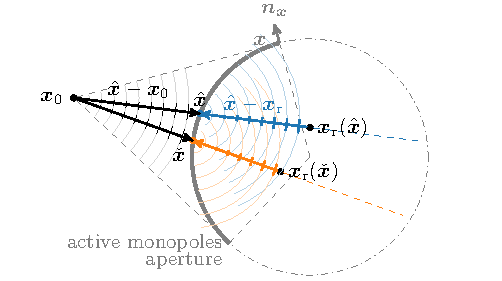
\includegraphics[width=85mm]{../graphics_ENG/spa_3d.pdf}
\end{plotfigures}
\caption{%3D-WFS.
Sound ray model for 3D WFS.
%
%Monopole bei $\xs$, angeordnet zu einem kugelförmigen Array, und eine
%virtuelle Punktquelle bei $\xp$.
Spherical array equipped with monopoles at positions $\xs$,
and a virtual point source at $\xp$.
%
%Die Sattelpunktsnäherung kann als akustisches Strahlenmodell interpretiert werden:
The stationary phase approximation can be interpreted as a
sound ray model\index{sound ray model}:
%
%nur der auf dem Direktpfad von virtueller Quelle zu Empfänger (Vektor $\xr - \xp$)
%auf der Hüllfläche liegende Monopol trägt maßgeblich zur
%Synthese des Schallfelds der virtuellen Quelle bei.
The direct path from the virtual source to the receiver
(cf. vector $\xr - \xp$)
intersects the spherical array at a certain position $\xs$.
Only the monopole at this position contributes significantly
to the synthesis of the sound field $p(\xr)$ of the virtual source.
%
%Für alle Punkte auf der Direktpfadverlängerung
%(beispielhaft ausgehend von $\hat{\bm{x}}$ entlang blau bzw. von $\check{\bm{x}}$
%entlang orange) ist die Synthese bei 3D-WFS amplitudenkorrekt.
All points on the direct path within $V$ (for example starting
from $\hat{\bm{x}}$ along the blue line and
from $\check{\bm{x}}$ along the orange line, respectively)
experience amplitude-correct synthesis for the 3D WFS case.
%
%Darstellung hier in 2D, man stelle sich eine Kugelkappe als
%Geometrie der aktiven Sekundärquellen vor, Empfängerpunkte innerhalb der Kugel.
For the 2D depiction here, imagine the geometry of the active
secondary monopole sources as a spherical cap, with receiver points
inside the sphere.
%
\cc
}
\label{fig:3DWFS_Schema}
\end{figure}



%Aus der Sattelpunktsnäherung lässt sich zudem schliessen,
%dass dieses lokal begrenzte Ergebnis
%maßgeblich von nur \textit{einem} Sekundärmonopol auf der Hüllfläche/-linie
%erzeugt wird.
The SPA theory further allows the deduction that only \textit{one}
secondary monopole has a physically meaningful impact on this local result.
%
%Er befindet sich an der Position $\xs$, wo der Direktpfad von virtueller
%Quelle $\xp$ zu Empfängerpunkt $\xr$ die Hülle durchstößt,
%vgl.~\myfig\ref{fig:3DWFS_Schema} und \ref{fig:25DWFS_Schema}.
This monopole is located at point $\xs$, where the direct path from the
virtual source position $\xp$ towards the probe point $\xr$ intersects
the secondary source hull, cf.~\myfigs\ref{fig:3DWFS_Schema} and
\ref{fig:25DWFS_Schema}.
%
%Dieses $\bm{x}$ ist für das Integral in \myeq\eqref{eq:KHIFarMono} ein
%Punkt stationärer Phase, der so genannt wird,
%weil in dessen Umgebung der Phasenterm des Integranden am wenigsten oszilliert.
For the integral in \myeq\eqref{eq:KHIFarMono}, this point $\bm{x}$
is a stationary phase point, which is defined as a point at which the phase
has a vanishing slope.
Therefore, the integrand in \eqref{eq:MonopolIntegral_3D} and
\eqref{eq:MonopolIntegral_25D} is free of local oscillations.
%
In \cite[Ch.~3.3]{Start1997_diss}, this specific point is called
the global `minimum phase' point.  % added in ENG version
%
%Genau dann gilt $\bm{\theta}_{\xs\text{-}\xr} = -\bm{\theta}_{\xs\text{-}\xp}$
%und damit für den Term in \myeq\eqref{eq:KHIFarMono} die Beziehung
%$\nxT \, \left(\bm{\theta}_{\xs\text{-}\xr} - \bm{\theta}_{\xs\text{-}\xp}\right)
%= - 2 \nxT \, \bm{\theta}_{\xs\text{-}\xp}$.
Then exactly $\bm{\theta}_{\xs\text{-}\xr} = -\bm{\theta}_{\xs\text{-}\xp}$ applies
and the term in \myeq\eqref{eq:KHIFarMono} results in
$\nxT \, \left(\bm{\theta}_{\xs\text{-}\xr} - \bm{\theta}_{\xs\text{-}\xp}\right)
= - 2 \cdot \nxT \, \bm{\theta}_{\xs\text{-}\xp}$.
%
%Dadurch vereinfacht sich das Integral, weil keine sekundären Dipolquellen mehr zur
%Synthese benötigt werden.
This considerably simplifies the integral, as the secondary dipole source type
is not necessary for synthesis.



% 2.5D-WFS
% please DO NOT rescale the figure and keep it single column
\begin{figure}
\centering
\begin{plotfigures}
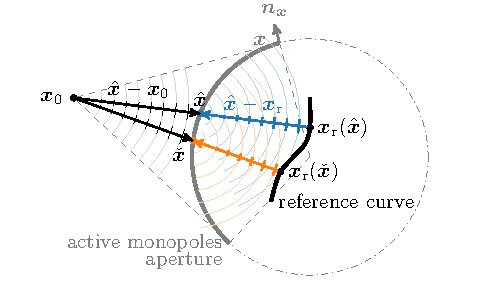
\includegraphics[width=85mm]{../graphics_ENG/spa_25d.pdf}
\end{plotfigures}
\caption{%2.5D-WFS. Alle Punkte und Vektoren in der gleichen Ebene.
Sound ray model for 2.5D WFS.
All points and vectors are assumed to lie in the same plane.
%
%Monopole bei $\xs$, angeordnet zu einem kreisförmigen Array, und eine
%virtuelle Punktquelle bei $\xp$.
Circular array equipped with monopoles at positions $\xs$,
and a virtual point source at $\xp$.
%
%Sattelpunktsnäherung für 2.5D-WFS:
The sound ray model $\xr - \xp$ determines the most significant monopole.
It is located at the point $\xs$ at which the ray intersects the secondary
source curve.
%entlang des in den Zuhörerbereich verlängerten Pfades $\xs - \xp$ trägt nur der
%Monopol am Hüllkontur-Durchstoßpunkt maßgeblich zum synthetisierten
%Schallfeld bei.
%
%Amplitudenkorrekte Synthese ist für genau einen Referenzpunkt
%$\xr(\xs)$ auf diesem Pfad möglich.
Amplitude-corrected synthesis is only possible for one receiver
position $\xr(\xs)$ lying on that ray.
%
%Umkehrschluss: Entlang einer in Grenzen wählbaren Referenzkurve mit den Punkten
%$\xr(\xs)$ -- in der Grafik angedeutet mit
%$\xr(\hat{\bm{x}})$ bzw. $\xr(\check{\bm{x}})$
%für die Monopole bei $\hat{\bm{x}}$ bzw.
%$\check{\bm{x}}$ -- findet sich für jeden Referenzpunkt genau eine Quelle $\xs$
%auf dem Pfad von virtueller Quelle zu Referenzpunkt.
%
Conversely, this means that a freely selectable reference curve
with points $\xr(\xs)$ -- in the graphics indicated with
$\xr(\hat{\bm{x}})$ and $\xr(\check{\bm{x}})$
for the monopoles at $\hat{\bm{x}}$ and $\check{\bm{x}}$, respectively -- can
be defined within certain limits, along which the synthesis can be corrected
in amplitude.
%
%Mittels Amplitudenkorrektur dieser Quelle $\xs$ (vgl.~\myeq\eqref{eq:Driving25D})
%gelingt amplitudenkorrekte
%Synthese entlang der gewählten Referenzkurve $\xr(\xs)$.
The respective monopoles are individually corrected in amplitude
according to \myeq\eqref{eq:Driving25D}.
%
\cc
}
\label{fig:25DWFS_Schema}
\end{figure}



%Beiträge zur Lösung mit potentiell anderen Punkten stationärer Phase
%-- unbrauchbare Spiegelreflexionen \cite{ZotterSchultz2020_White} -- werden
%formal mit der Maximum-Operation
%\begin{align}
%\label{eq:SecSrcSel}
%2\cdot\mathrm{max}\{-\nxT \, \bm{\theta}_{\xs\text{-}\xp}, 0\}
%\end{align}
%unterdrückt.
There might be other potential points that satisfy the stationary phase
condition.
However, the SPA evokes zero amplitude for these specular reflections, cf.
\cite{ZotterSchultz2020_White}.  % better stated in ENG version
The formal operator
\begin{align}
\label{eq:SecSrcSel}
2\cdot\mathrm{max}\{-\nxT \, \bm{\theta}_{\xs\text{-}\xp}, 0\}.
\end{align}
is used in the driving function \eqref{eq:Driving3D} to cover this property.
%Dieses sattelpunktsnäherung-inhärente Kriterium ist identisch mit dem sogenannten
%\textit{secondary source selection criterion}
%\index{secondary source selection criterion} \cite{Nicol1999, Spors2007b, Spors2008a},
%welches bei WFS-Herleitungen gesondert eingeführt wurde.
This criterion inherent to the SPA is identical to the
`secondary source selection criterion'\index{secondary source selection criterion}
\cite{Nicol1999, Spors2007b, Spors2008a}, which was initially introduced
separately from the SPA.
%
%Es ist auch im Kontext der HF-BEM bekannt und sorgt dafür,
%dass bei der Synthese keine Monopole aktiv sind,
%deren Wellenausbreitung in der Zuhörerfläche jener der virtuellen Quelle
%entgegenlaufen.
It is also used in the HF-BEM to deactivate monopoles with wave propagation
opposite to that of the virtual source within the listening area.
%
%In optischer Analogie sind nur die Monopole einer sinnvollerweise konvexen
%Hüllfläche aktiv, von denen aus eine direkte Sicht auf die virtuelle Quelle
%möglich ist, vgl.~\myfig\ref{fig:3DWFS_Schema}.
In an optical analogy, only those monopoles of a convex hull are activated when
there is a direct line of sight to the virtual source,
cf.~\myfig\ref{fig:3DWFS_Schema}.



%\subsection{WFS-Ansteuerung im Frequenzbereich}
\subsection{WFS Driving Functions in the Frequency Domain}

%Die Ergebnisse in \myeq\eqref{eq:pStat3D} und \eqref{eq:pStat25D} aus der
%Sattelpunktsnäherung besagen, dass zur Erzeugung des Schalldrucks
%an einem spezifizierten Punkt $\xr$ nur ein Monopol maßgeblich beteiligt ist,
%was sich als Schallstrahlenmodell interpretieren lässt.
The derivations from the SPA leading to
\myeqn\eqref{eq:pStat3D} and \eqref{eq:pStat25D}
suggest that only one monopole is significantly involved in generating the
sound pressure at a specified point $\xr$.
This can be interpreted as a sound ray model.
%
%Da die Erzeugung des korrekten Schalldrucks für mehrere Empfängerpunkte im Fokus
%der WFS steht, also mehrere Schallstrahlen zur korrekten Wellenfrontkrümmung
%\index{Wellenfrontkrümmung}
WFS aims to achieve the correct sound pressure for multiple receiver points.
This requires multiple sound rays that correctly contribute to an intended
wavefront curvature\index{wavefront curvature}.
%beitragen sollen, müssen die \myeqn\eqref{eq:pStat3D}, \eqref{eq:pStat25D},
%\eqref{eq:SecSrcSel} und
%\eqref{eq:KHIFarMono} sinnvoll verknüpft werden, damit für die Syntheseintegrale
%\eqref{eq:MonopolIntegral_3D}, \eqref{eq:MonopolIntegral_25D}
%die benötigten WFS-Ansteuerungsfilter angegeben
%werden können.
Therefore, \myeqn\eqref{eq:pStat3D}, \eqref{eq:pStat25D}, as well as
the secondary source selection criterion \eqref{eq:SecSrcSel},
and \eqref{eq:KHIFarMono} must be linked in a meaningful way so that
the required WFS driving functions can be specified for the synthesis integrals
\eqref{eq:MonopolIntegral_3D}, \eqref{eq:MonopolIntegral_25D}.
%
%Dem impliziten Lösungsansatz folgend, wird dazu die erste
%geschweifte Klammer in \myeq\eqref{eq:KHIFarMono} mit \eqref{eq:pStat3D} bzw.
%\eqref{eq:pStat25D} verglichen.
The implicit solution approach suggests a coefficient comparison for the
first curly bracket term in \myeq\eqref{eq:KHIFarMono} vs. the SPA results
\eqref{eq:pStat3D} and \eqref{eq:pStat25D}, respectively.
%
%Für eine breitbandige Ansteuerung resultiert der Filter-Frequenzgang
%für den 3D-Synthese-Fall
For broadband control, the driving function for 3D synthesis is
%
\begin{align}
D_\text{3D}(\xp,\xs,\omega) = 2\im\wc \mathrm{max}\{-\nxT \, \bm{\theta}_{\xs\text{-}\xp}, 0\} \, G(r_{\xs\text{-}\xp},\omega)
\label{eq:Driving3D}
\end{align}
%
%und der Filter-Frequenzgang für den 2.5D-Synthese-Fall, vgl. \cite{Deregowski1983,Bleistein1986}
and the driving function for 2.5D synthesis is,
cf. \cite{Deregowski1983,Bleistein1986}
%
\begin{align}
D_\text{2.5D}(\xp, \xs, \xr,\omega) = \underbrace{D_\text{3D}(\xp,\xs,\omega)}_{\text{3D WFS driving function \eqref{eq:Driving3D}}} \times\label{eq:Driving25D}\\
\underbrace{\sqrt{\frac{2\pi}{\im\wc} r_{\xs\text{-}\xr}}
\sqrt{\frac{r_{\xs\text{-}\xp}}{r_{\xs\text{-}\xr} + r_{\xs\text{-}\xp}}}}_{\text{reciprocal factors of \eqref{eq:pStat25D}}}\nonumber
\end{align}
%
%für jeden Monopol $\xs$.
individually for each secondary monopole source at position $\xs$.
%
%Bei 2.5D-Synthese sorgen die reziproken Wurzel-Faktoren
%für die Kompensation der bei der Sattelpunktsnäherungslösung in \myeq\eqref{eq:pStat25D}
%entstandenen Abweichung.
The 2.5D driving function requires the use of two reciprocal square root terms
to compensate for the deviations occurring in the 2.5D SPA result
\myeq\eqref{eq:pStat25D}.
%
%Der erste Wurzel-Ausdruck in \myeq\eqref{eq:Driving25D} ist ein Filter und
%kompensiert den Umstand,
%dass sich die 2D-Hüllkontur spektral anders verhält als die 3D-Hüllfläche,
The first square root expression in \myeq\eqref{eq:Driving25D} represents a
filter that compensates for the spectral differences between the 2D curve
and the 3D surface.
%während die zweite Wurzel als Gainwert die Amplitudenabnahme der 3D-Primärquelle
%bezüglich der 2D-Zuhörerebene normalisiert, vgl. \cite[Kap.~4.1.3]{Firtha2019_diss}.
The second square root term acts as a gain factor that normalises
the level loss of the 3D virtual source in relation to the 2D listening area,
cf. \cite[Ch.~4.1.3]{Firtha2019_diss}.
%
%Letzteres wird im Folgenden als Amplitudenkorrektur bezeichnet.
The latter is referred to as amplitude correction.
%
%Wenn $r_{\xs\text{-}\xp} \gg r_{\xs\text{-}\xr}$ eingehalten wird, weist die
%synthetisierte Welle eine verschwindende Wellenkrümmung bei $\xr$ auf und
%der zweite Wurzel-Ausdruck geht gegen Eins.
Under the condition $r_{\xs\text{-}\xp} \gg r_{\xs\text{-}\xr}$ the
synthesised wave exhibits a negligible wavefront curvature; the
second square root term approaches one.
%
%Dies kann für die 2.5D-WFS als ebenes Wellenmodell genutzt werden.
This can be used as a virtual plane wave model within the 2.5D WFS.



%Die für 2.5D-WFS erforderliche Amplitudenkorrektur ist nur möglich für Punktpaare
%stationärer Phase:
Amplitude correction for 2.5D WFS is only possible for
stationary phase point pairs:
%
%Für ein bestimmtes $\xs$ kann ein bestimmtes $\xr$
%festgelegt werden, für das die Synthese amplitudenkorrekt\index{amplitudenkorrekte Synthese}
%sein soll, vgl.~\myfig\ref{fig:25DWFS_Schema}, \cite[Kap.~3]{Start1997_diss}, \cite[Kap.~4]{Firtha2019_diss}.
For a given $\xs$, amplitude-corrected synthesis allows the selection
of exactly one dedicated $\xr$ along the specific sound ray,
cf.~\myfig\ref{fig:25DWFS_Schema},
\cite[Ch.~3]{Start1997_diss} and
\cite[Ch.~4]{Firtha2019_diss}.
%
%Der 3D-Fall ist amplitudenkorrekt für alle $\xr$, falls die oben eingeführten
%Näherungsbedingungen eingehalten werden, vgl.~\myfig\ref{fig:3DWFS_Schema}.
Assuming the above approximations are valid, the 3D WFS provides
amplitude-correct synthesis for all $\xr$, cf.~\myfig\ref{fig:3DWFS_Schema}.



%Die Lösungen in \myeq\eqref{eq:Driving3D}, \eqref{eq:Driving25D}
%für die Syntheseintegrale
%\eqref{eq:MonopolIntegral_3D}, \eqref{eq:MonopolIntegral_25D}
%sind nur dann eine valide Näherung, wenn -- neben Einhaltung
%der Fernfeld-/Hochfrequenznäherung --
%sowohl die Wellenlänge als auch die Wellenfrontkrümmung in Nähe der Hülle
%deutlich kleiner als die räumliche Ausdehnung der aktiven Hüllfläche bzw. -kontur
%(sogenannte Apertur\index{Apertur}) sind;
%dies folgt aus der Theorie der Kirchhoff- bzw.
%Fresnel-Kirchhoff-Beugung, für die WFS detailliert diskutiert in
%\cite{Schultz2016_diss, Firtha2019_diss}.
The solutions
\eqref{eq:Driving3D} and \eqref{eq:Driving25D}
for the synthesis integrals
\eqref{eq:MonopolIntegral_3D} and \eqref{eq:MonopolIntegral_25D}
require compliance with the far-field/high-frequency approximation.
This means that the wavelength and the local wavefront curvature
near the surface/curve must be considerably smaller than
the spatial extent of the active part of the surface/curve,
i.e. the aperture\index{aperture}.
This follows from the Fresnel-Kirchhoff diffraction theory,
for WFS applications discussed, e.g. in \cite{Schultz2016_diss,
Firtha2019_diss}.



% please DO NOT rescale the figure and keep it double column
\begin{figure*}
\centering
\begin{plotfigures}
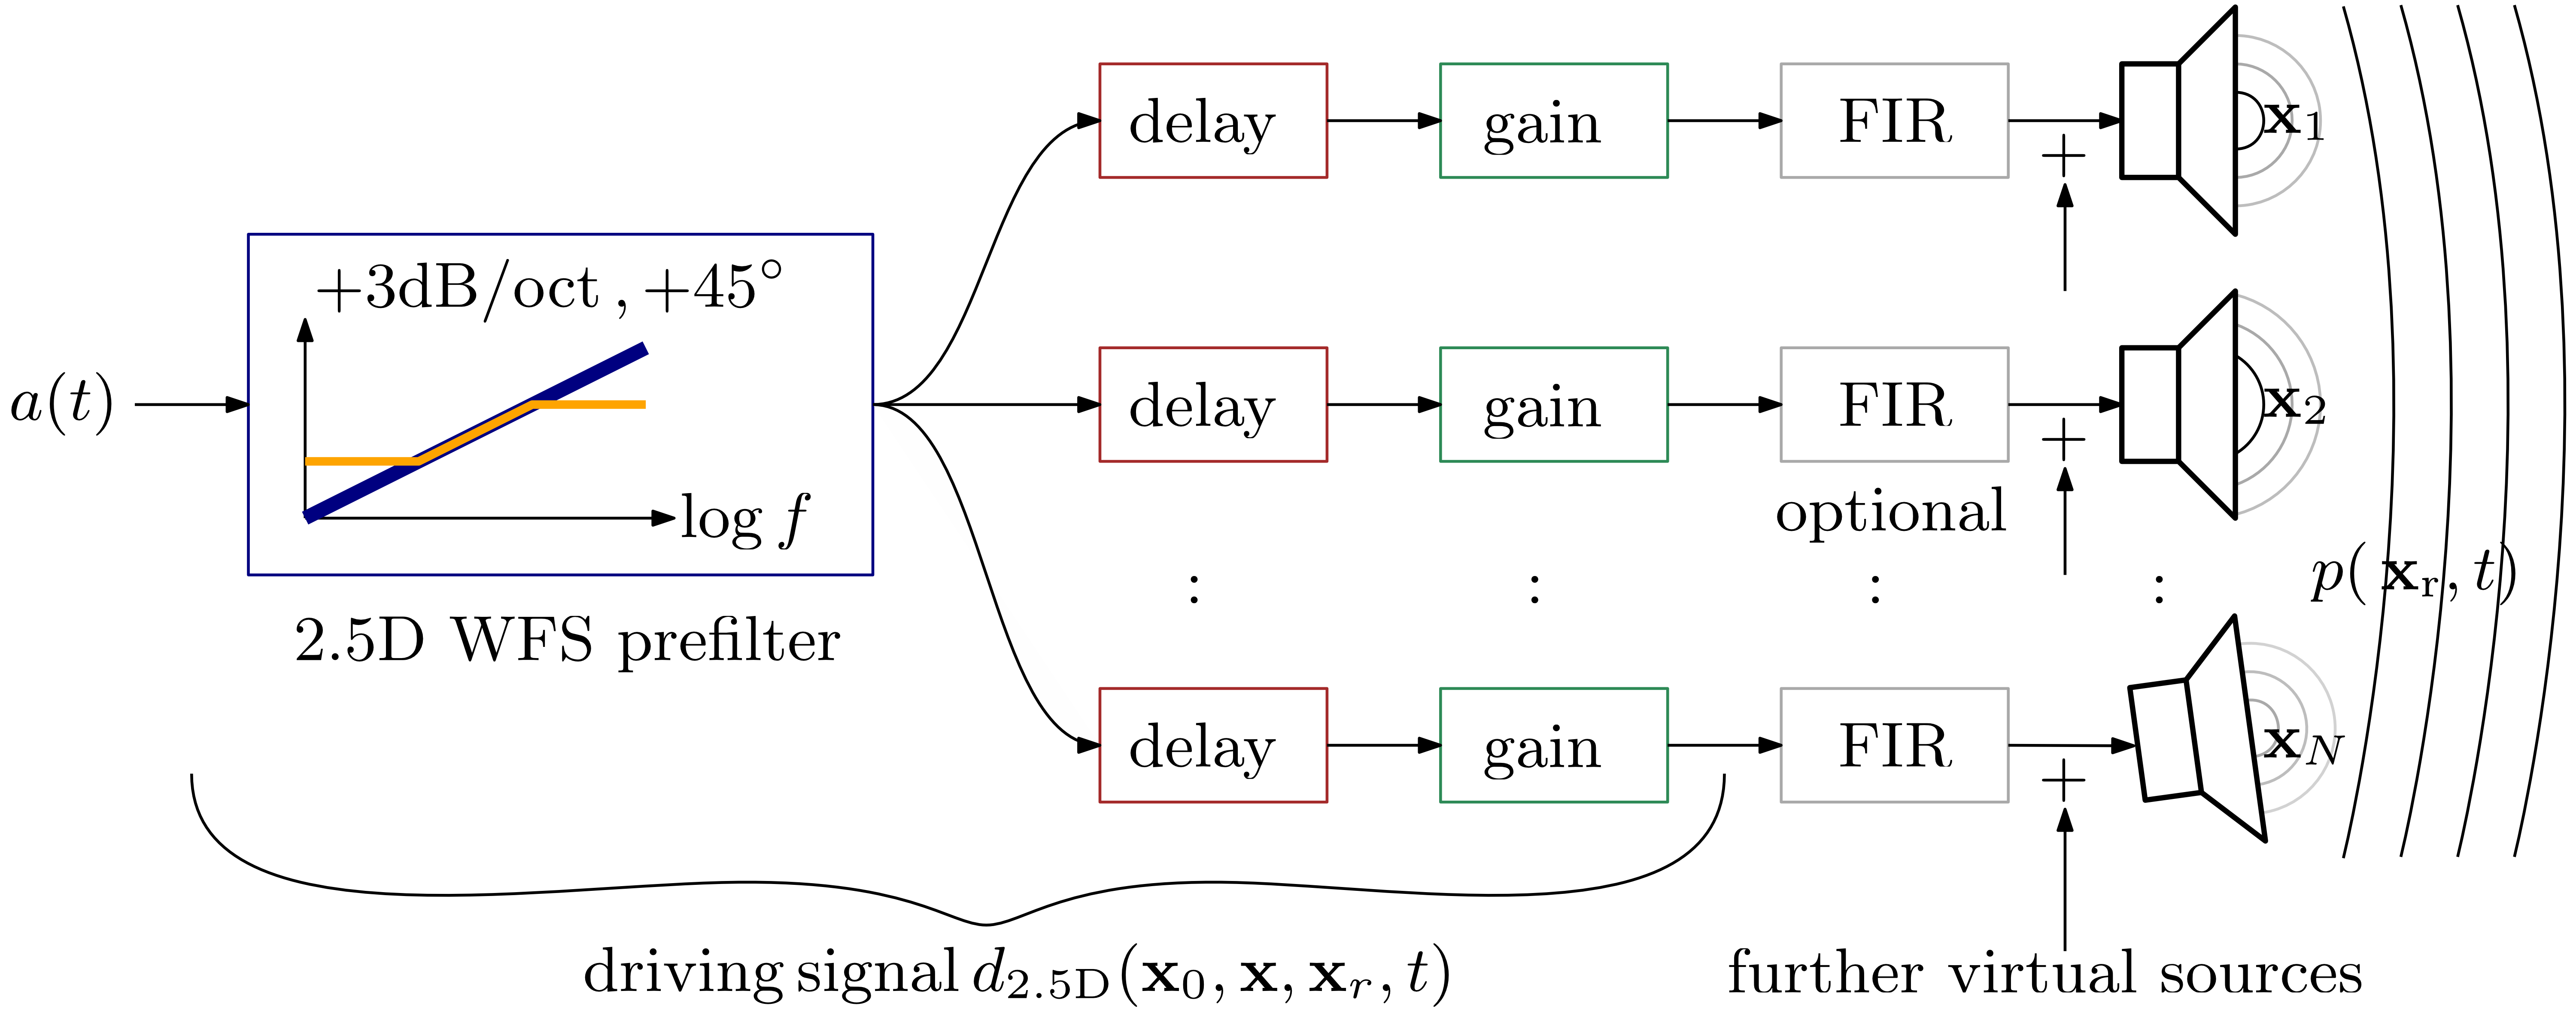
\includegraphics[width=145mm]{../graphics_ENG/WFS_Blockdiagramm.png}
\end{plotfigures}
\caption{%Signalfluss von Audiosignal $a(t)$ zu Schalldruck $p(\xr, t)$
%für die modellbasierte 2.5D-WFS.
Signal flow from audio signal $a(t)$ to sound pressure $p(\xr, t)$ for the
model-based 2.5D WFS.
%Das Audio-Eingangssignal $a(t)$ wird zunächst mit dem sogenannten 2.5D-WFS-Vorfilter
%\index{WFS-Vorfilter} gefiltert.
First, the audio input signal $a(t)$ is filtered with the
WFS prefilter\index{WFS prefilter}.
%
%Danach folgen lautsprecherindividuelles Delay und Gain $\gain_\text{2.5D}$, welche sich aus der
%Parametrik der virtuellen Quelle und Array-Geometrie ergeben,
%siehe Treiberfunktion im Zeitbereich
%in \myeq\eqref{eq:h25d_time}.
This is followed by applying loudspeaker-specific delay and gain,
which result from the parameters of the virtual source and the
array geometry, cf. the driving signals \myeq\eqref{eq:h25d_time}.
%
%Die akustische Superposition von komplex gewichteten, akustischen Übertragungsfunktionen
%$G(r_{\xs\text{-}\xr})$ führt zum Schalldruck $p(\xr, t)$.
The acoustic superposition of the individual sound fields from
the loudspeakers results in the sound pressure $p(\xr, t)$.
%
%Optionale Schallfeldoptimierung erfolgt typisch mit
%lautsprecherindividuellen FIR-Filtern.
Optional sound field optimisation is usually carried out using
loudspeaker-specific FIR filters.
%
%Die Superposition von Ansteuerungssignalen erlaubt die Synthese mehrerer virtueller
%Quellen gleichzeitig.
Superimposing driving signals enables multiple virtual sources to
be synthesised simultaneously.
%
\cc
}
\label{fig:WFS_Blockdiagramm}
\end{figure*}



%\subsection{WFS-Ansteuerung im Zeitbereich}
\subsection{WFS Driving Signals in the Time Domain}
\label{sec:WFS_Ansteuerung_im_Zeitbereich}

%WFS-Signalverarbeitung im Zeitbereich erfordert pro Lautsprecher
%einen individuellen Gain- und Delaywert, sowie ein spezielles Hochpassfilter,
%vgl.~\myfig\ref{fig:WFS_Blockdiagramm} für die 2.5D-WFS.
WFS signal processing in the time domain requires individual gain and
delay for each loudspeaker, as well as a special high-pass filter,
cf.~\myfig\ref{fig:WFS_Blockdiagramm} for the case of 2.5D WFS.
%
%Dies sind vergleichsweise einfache Operationen in der Signalverarbeitung.
These are elementary signal processing operations.
%
%Wegen Präzision und Flexibilität sollte die Umsetzung mit Digitaltechnik
%erfolgen.
They should be implemented using digital technology to ensure
precision and flexibility.
%
%Das WFS-Ansteuerungsfilter im Zeitbereich, also die
%Filter-Impulsantwort für den Monopol an der
%Position $\xs$, wird für 3D-Synthese mit
The WFS driving signal
for the secondary monopole source at $\xs$ is
\begin{align}
d_\text{3D}(\xp,\xs, t) =
\underbrace{\gain_\text{3D}(\xp,\xs)}_{\text{gain}} \cdot
\underbrace{\delta(t-\frac{r_{\xs\text{-}\xp}}{c})}_{\text{delay}} \,\ast_t\,
\underbrace{h_\text{3D,Pre}(t)}_{\text{prefilter}}
\end{align}
for 3D synthesis
%und für 2.5D-Synthese mit
and
\begin{align}
d_\text{2.5D}(\xp,\xs,\xr, t) =
&\gain_\text{2.5D}(\xp,\xs,\xr) \times\nonumber\\
&\delta(t-\frac{r_{\xs\text{-}\xp}}{c}) \,\ast_t\,
h_\text{2.5D,Pre}(t)
\label{eq:h25d_time}
\end{align}
for 2.5D synthesis, respectively.
%beschrieben.
%
%Die Faltungsoperation $\ast_t$ bezüglich der Zeit $t$ ist die
%korrespondierende Operation zur Multiplikation von $\omega$-abhängigen
%Frequenzgängen.
According to the Fourier transform theory, the convolution operation,
denoted by $\ast_t$, is the time-domain equivalent of the frequency-domain
spectrum multiplication.



%Die $\im\frac{\omega}{c}$-unabhängigen Terme in den Filter-Frequenzgängen
%in den \myeqn\eqref{eq:Driving3D}, \eqref{eq:Driving25D}
The expressions that are independent of $\im\frac{\omega}{c}$
in the driving functions \eqref{eq:Driving3D}, \eqref{eq:Driving25D}
%
\begin{align}
&\gain_\text{3D}(\xp,\xs) = 2 \, \mathrm{max}\{-\nxT \, \bm{\theta}_{\xs\text{-}\xp}, 0\} \, \frac{1}{4\pi \, r_{\xs\text{-}\xp}}\\
%
&\gain_\text{2.5D}(\xp,\xs,\xr) =
\sqrt{2\pi}
\sqrt{\frac{r_{\xs\text{-}\xr} \cdot r_{\xs\text{-}\xp}}{r_{\xs\text{-}\xr} + r_{\xs\text{-}\xp}}}
\cdot \gain_\text{3D}(\xp,\xs)\nonumber\\
&={\frac{1}{\sqrt{2\pi}}}
\sqrt{\frac{r_{\xs\text{-}\xr}}{r_{\xs\text{-}\xr} + r_{\xs\text{-}\xp}}} \frac{1}{\sqrt{r_{\xs\text{-}\xp}}}
\,\mathrm{max}\{-\nxT \, \bm{\theta}_{\xs\text{-}\xp}, 0\}
\end{align}
%
%verhalten sich bezüglich der Fourier-Transformation wie konstante Faktoren, treten
%daher im Frequenz- und Zeitbereich gleich auf.
constitute constant factors for the Fourier transform, therefore being present
equally in the frequency and time domains.
%
%Diese stellen die lautsprecherindividuellen Gewichte (\textit{gain}) für den
%3D-~bzw.~2.5D-Fall dar.
They represent the individual weighting factors (\textit{gain}) of the
loudspeakers for the 3D and 2.5D case, respectively.
%
%Im 3D-Fall ist das Gewicht pro Lautsprecher nur von der Position $\xp$  der
%virtuellen Punktquelle und natürlich von der Lautsprecherposition $\xs$ abhängig.
In the case of 3D, the gain per loudspeaker is calculated using the virtual
source position $\xp$, and the loudspeaker position $\xs$.
%
%Im 2.5D-Fall ergibt sich eine zusätzliche Abhängigkeit zu genau dem Empfängerpunkt
%$\xr(\xs)$, für den eine amplitudenkorrekte Synthese realisiert werden soll,
%vgl.~\myfig\ref{fig:25DWFS_Schema}.
In the case of 2.5D, the dependency of the amplitude-corrected receiver points
$\xr(\xs)$ must also be taken into account, cf.~\myfig\ref{fig:25DWFS_Schema}.



%In den Filter-Frequenzgängen in den \myeqn\eqref{eq:Driving3D}, \eqref{eq:Driving25D}
%resultiert für den in $G(r_{\xs\text{-}\xp},\omega)$ (vgl.~\myeq\eqref{eq:G03D})
%auftretenden komplexen Zeiger
%$\e^{-\im\wc r_{\xs\text{-}\xp}}$
%die zeitliche Korrespondenz
%\begin{align}
%\e^{-\im\wc r_{\xs\text{-}\xp}}
%\quad\Laplace\quad
%\delta\left(t-\frac{r_{\xs\text{-}\xp}}{c}\right)
%\end{align}
%aus inverser Fourier-Transformation (angedeutet mit dem Operator $\,\Laplace\,$).
The driving functions \eqref{eq:Driving3D}, \eqref{eq:Driving25D} further
include the complex exponential
$\e^{-\im\wc r_{\xs\text{-}\xp}}$ from the spectrum
$G(r_{\xs\text{-}\xp},\omega)$, cf.~\myeq\eqref{eq:G03D}.
With the operator symbol $\,\Laplace\,$ for the inverse Fourier transform,
the correspondence
\begin{align}
\e^{-\im\wc r_{\xs\text{-}\xp}}
\quad\Laplace\quad
\delta\left(t-\frac{r_{\xs\text{-}\xp}}{c}\right)
\end{align}
is written.
%
%Dies liefert den um
%$\tau_\text{Delay}=\frac{r_{\xs\text{-}\xp}}{c}$
%verzögerten Dirac-Impuls
%$\delta(t)$.
Hence, in the time domain, this provides the Dirac delta function
$\delta(t)$ shifted by $\tau_\text{Delay}=\frac{r_{\xs\text{-}\xp}}{c}>0$.
%
%Es handelt sich somit um eine Verzögerung (\textit{delay}) und
%bildet die von der Schallgeschwindigkeit $c$ abhängige Laufzeit des Schalls
%von der virtuellen Quelle bei $\xp$ zum jeweilig betrachteten Lautsprecher bei
%$\xs$ ab.
This represents a \textit{delay} that encodes the propagation time of the sound
from the virtual source at $\xp$ to the specific loudspeaker at $\xs$, which
naturally depends on the speed of sound $c$.



%Aus den \myeqn\eqref{eq:Driving3D}, \eqref{eq:Driving25D} sind nun noch die
%$\im\frac{\omega}{c}$-abhängigen Terme
The remaining expressions for the 3D and 2.5D cases
%
\begin{align}
&H_\text{3D,Pre}(\omega) = \im\frac{\omega}{c} \quad\Laplace\quad h_\text{3D,Pre}(t)
\label{eq:Prefilter3D}\\
%
&H_\text{2.5D,Pre}(\omega) = \frac{\im\frac{\omega}{c}}{\sqrt{\im\frac{\omega}{c}}} = \sqrt{\im\frac{\omega}{c}} \quad\Laplace\quad h_\text{2.5D,Pre}(t)
\label{eq:Prefilter25D}
\end{align}
%
in \myeqn\eqref{eq:Driving3D}, \eqref{eq:Driving25D}
are dependent from $\im\wc$.
%für den 3D-~bzw.~2.5D-Fall zu diskutieren.
%
%Diese Frequenzgänge beschreiben Hochpässe, die den inhärenten
%spektralen Tiefpasscharakter der Hüllfläche bzw. -kontur kompensieren.
These frequency responses describe high-pass filters to counteract the
inherent low-pass characteristics of the secondary source surface and
secondary source curve, respectively.
%
%Im 3D-Fall hat der kompensierende Hochpass eine Flanke von $+6$\,dB/Oktave mit
%$+90^\circ$ konstantem Phasenverlauf, im 2.5D-Fall hat das kompensierende Filter
%eine Flanke von $+3$\,dB/Oktave mit $+45^\circ$ konstanter Phase.
For 3D WFS, the compensating high-pass filter has a slope of $+6$\,dB/octave with
a constant phase of $+90^\circ$ (i.e. a differentiator),
whereas for 2.5D WFS, the high-pass filter features
a $+3$\,dB/octave slope and $+45^\circ$ constant phase
(i.e. a half-differentiator).
%
%Da die Hochpassfilter in den \myeqn\eqref{eq:Prefilter3D}, \eqref{eq:Prefilter25D}
%unabhängig von der virtuellen Quelle sind, erscheint es ganz vernünftig,
%das Audio-Eingangssignal $a(t)$ damit vorzufiltern
Since the high-pass filter %\myeqn\eqref{eq:Prefilter3D}, \eqref{eq:Prefilter25D}
is independent of the virtual source, it is reasonable to filter the audio
input signal $a(t)$ with it first -- hence the commonly used term
`WFS prefiltering'\index{WFS prefiltering} --
%-- dies führt auf den
%oft benutzten, englischen Begriff
%\textit{WFS pre-filtering}\index{WFS pre-filtering} -- und
%erst danach die lautsprecherindividuellen Verzögerungen und Gewichte
%auf das vorgefilterte Signal anzuwenden.
before applying the loudspeaker-specific delays and gain factors.
%
%\myfig\ref{fig:WFS_Blockdiagramm} verdeutlicht die beschriebenen
%Verarbeitungsschritte in einem Signalflussgraphen.
\myfig\ref{fig:WFS_Blockdiagramm} illustrates the described
processing steps in a signal flow graph.



%Das Schallfeld -- genauer die räumliche Ausbreitung der Wellenfront über die
%Zeit -- einer virtuellen Quelle mit der Ansteuerung des Audiosignals
%$a(t) \,\,\laplace\,\, A(\omega)$
%wird mittels der WFS also synthetisiert, indem die lautsprecherindividuelle
%Faltung $a(t) \ast_t d(t)$ (elektrische Ansteuerung) realisiert wird und
%sich die ausbreitenden Schallfelder der Lautsprecher zur gewünschten Wellenfront
%überlagern (akustisches Resultat).
In conclusion, the WFS of a virtual source with its audio signal
$a(t) \,\,\laplace\,\, A(\omega)$ goes by the loudspeaker-specific
convolution $a(t) \ast_t d(t,\xs)$ with the driving signal $d(t,\xs)$
(i.e. the active electrical control per loudspeaker), resulting in the
superposition of the loudspeaker sound fields towards the intended
wavefront (i.e. the acoustic result due to interference).
%
%In der Praxis wird die Faltung $a(t) \ast_t d(t)$, wie oben diskutiert,
%oft aufgeteilt in Hochpassfilter, Delay und Gain.
In practice, as discussed above, the convolution $a(t) \ast_t d(t,\xs)$
is often split into the signal processing blocks
prefilter, delay and gain.



%\section{Simulationen für die WFS einer virtuellen Punktquelle}
\section{Simulations for the WFS of a Virtual Point Source}
\label{sec:WFS_PointSource_Simulationen}

%In diesem Abschnitt illustrieren Ergebnisse von numerischen Simulationen die
%Funktionsweise und die wichtigsten Eigenschaften von 2.5D-WFS,
This section presents the results of numerical simulations, which
illustrate the functionality and key properties of the 2.5D WFS,
cf. \cite{Berkhout1993_JASA,Boone1995_JAES,Start1997_diss,Spors2010a}.
%
%Die Simulationen beruhen auf dem obigen Formelapparat für 2.5D-WFS
These simulations are based on the mathematical formulae for
2.5D WFS described above.
%und können z.B. mit der Sound Field Synthesis
%Toolbox \cite{Winter2019dagaposter}\footnote{\url{https://github.com/sfstoolbox}}
%und der Referenzimplementierung zu diesem
%Kapitel\footnote{\url{https://github.com/spatialaudio/wfs_chapter_hda}}
%nachvollzogen und durchgeführt werden.
They can be performed with the accompanying reference
implementation\footnote{\url{https://github.com/spatialaudio/wfs_chapter_hda}}
and the
Sound Field Synthesis Toolbox\footnote{\url{https://github.com/sfstoolbox/sfs-python}}.
%\cite{Winter2019dagaposter}.  % omit DAGA poster/paper in ENG version
%
%Für alle folgenden Simulationen ist die Schallgeschwindigkeit $c=343$\,m/s.
The simulations use the speed of sound $c=343$\,m/s.
%
%Zunächst werden monofrequente Schallfelder in den
%%\myfig\ref{fig:wfs25d_lineSSD},~\ref{fig:wfs25d_circSSD},~\ref{fig:wfs25d_lineSSD_truncation},~\ref{fig:wfs25d_lineSSD_aliasin%g},~\ref{fig:wfs25d_lineSSD_polar_plot_overlay},~\ref{fig:wfs25d_circSSD_aliasing},
%\myfig\ref{fig:wfs25d_lineSSD} bis \ref{fig:wfs25d_circSSD_aliasing},
%und anschließend
%%in fig:td_0m_noaliasing \myfig\ref{fig:td_-1m},~\ref{fig:td_0m},~\ref{fig:td_1m}
%impulsartige Schallfelder im Zeit- und Frequenzbereich
%in den \myfig\ref{fig:td_0m_noaliasing} bis \ref{fig:td_1m}
%diskutiert.
First, single-frequency sound fields are discussed by means of the
\myfigs\ref{fig:wfs25d_lineSSD}--\ref{fig:wfs25d_circSSD_aliasing},
followed by broadband sound fields in the time and frequency domains
using the \myfigs\ref{fig:td_0m_noaliasing}--\ref{fig:td_1m}.



%\subsection{Nah-/Fernfeld vs. Wellenfront-/Abstrahlsynthese}
\subsection{Nearfield/Farfield vs. Wavefront/Radiation Synthesis}

%Vorangestellt sei noch, dass sich die folgende Diskussion des Konzepts der Fraunhofer-
%bzw. Fresnel-Region \cite[Kap.~26]{Skudrzyk1971} bedient:
%It should be noted in advance that
The following discussion refers to the Fraunhofer and Fresnel regions
\cite[Ch.~26]{Skudrzyk1971}.
%Interferenzeffekte
%sind an verschiedenen Empfängerpunkten näherungsweise analytisch zugänglich und
%damit aus Formeln heraus interpretierbar.
The interference phenomena that occur in these regions can be analysed
approximately using equations for certain receiver points.
%
%Das Konzept wird hier stark vereinfacht benutzt und die Fraunhofer-Region mit dem
%Fernfeld\index{Fernfeld} bzw. die Fresnel-Region mit dem
%Nahfeld\index{Nahfeld} endlicher Lautsprecherarrays gleichgesetzt.
Although simplified, it is essentially true that, for finite-size
loudspeaker arrays,
the Fraunhofer region corresponds to the far field\index{far field},
while the Fresnel region corresponds to the near field\index{near field}.
%
%Für eine endlich große Quelle mit größter Abmessung $l$ (d.h. die aktive Apertur)
%befindet sich ein Messpunkt mit Quellenabstand $R$ im Fernfeld, wenn die
%drei Kriterien
For a sound source with the largest dimension $l$ (i.e. the active aperture),
a probe point is considered to be in the far field at a distance $R$ if the
following three conditions are met \cite[Ch.~3.5.4]{Moeser2009_book}:
%a) $R \gg l$,
%b) $\frac{R}{l} \gg \frac{l}{\lambda}$ und
%c) $R \gg \lambda$ (ähnlich der oben gemachten Fernfeld-/Hochfrequenznäherung
%$\frac{\omega}{c} R \gg 1$) erfüllt werden, vgl. \cite[Kap.~3.5.4]{Moeser2009_book}.
a) $R \gg l$,
b) $\frac{R}{l} \gg \frac{l}{\lambda}$ and
c) $R \gg \lambda$ (the latter is similar to the far-field/high-frequency
approximation $\frac{\omega}{c} R \gg 1$).
%
%Würde der Schalldruck um das mit den Treiberfunktionen angesteuerte,
%endliche Lautsprecherarray auf einer Kugeloberfläche erfasst, würde sich ab einer
%bestimmten Entfernung -- der aus den Bedingungen a) bis c) resultierenden,
%frequenzabhängigen Nah-/Fernfeldgrenze -- eine
%frequenzabhängige
%Fernfeldrichtcharakteristik\index{Fernfeldrichtcharakteristik} ausprägen, welche in
%noch weiterer Entfernung vom Array
%$6$\,dB-Pegelverlust pro Entfernungsverdopplung verzeichnet.
Now, consider a finite-length loudspeaker array that is controlled using
WFS driving signals.
Conditions a), b) and c) imply a frequency-dependent near-field/far-field
transition.
The resulting sound pressure, measured at a far-field distance along a
spherical surface reveals the frequency-dependent
far-field directivity\index{far-field directivity}.
In the far field, a $6$\,dB level loss per doubling of distance holds.



%Bei Schallfeldsynthese wird gezielt Interferenz erzeugt, so dass sich im Nahfeld des
%Lautsprecherarrays die gewünschte Wellenfrontkrümmung mit charakteristischer
%Amplitudenabnahme ergibt.
Sound field synthesis purposely generates interference so that the desired
wavefront curvature with characteristic amplitude decay is realised in the
near field of the loudspeaker array.
%
%Hingegen wird bei Abstrahlsynthese (\textit{beam forming}) gezielt mit
%Interferenz gearbeitet, um eine gewünschte Fernfeldrichtcharakteristik zu
%realisieren.
In contrast, radiation synthesis uses interference to achieve
a desired far-field directivity (cf. beamforming).
%
%Die Wellenfrontkrümmung im Fernfeld einer Quelle ist wegen des $6$\,dB-Pegelverlustes
%immer punktquellenartig,
%
%auch wenn in einem räumlich begrenzten Bereich in sehr weitem Abstand zur Quelle
%diese Krümmung verschwindend klein erscheinen kann.
Due to the $6$\,dB level loss, the wavefront curvature in the far field
always corresponds to that of a point source.
However, when considering a small local area at a great distance
from the source, the curvature becomes imperceptible.
%
%Dieser Effekt wird genau bei der Modellierung der virtuellen ebenen Welle mittels
%einer sehr weit entfernten virtuellen Punktquelle ausgenutzt.
This effect can be exploited precisely for modelling a virtual plane wave
by using a virtual point source located far away.



% please DO NOT rescale the figure and keep it single column
\begin{figure}
\centering
\begin{plotfigures}
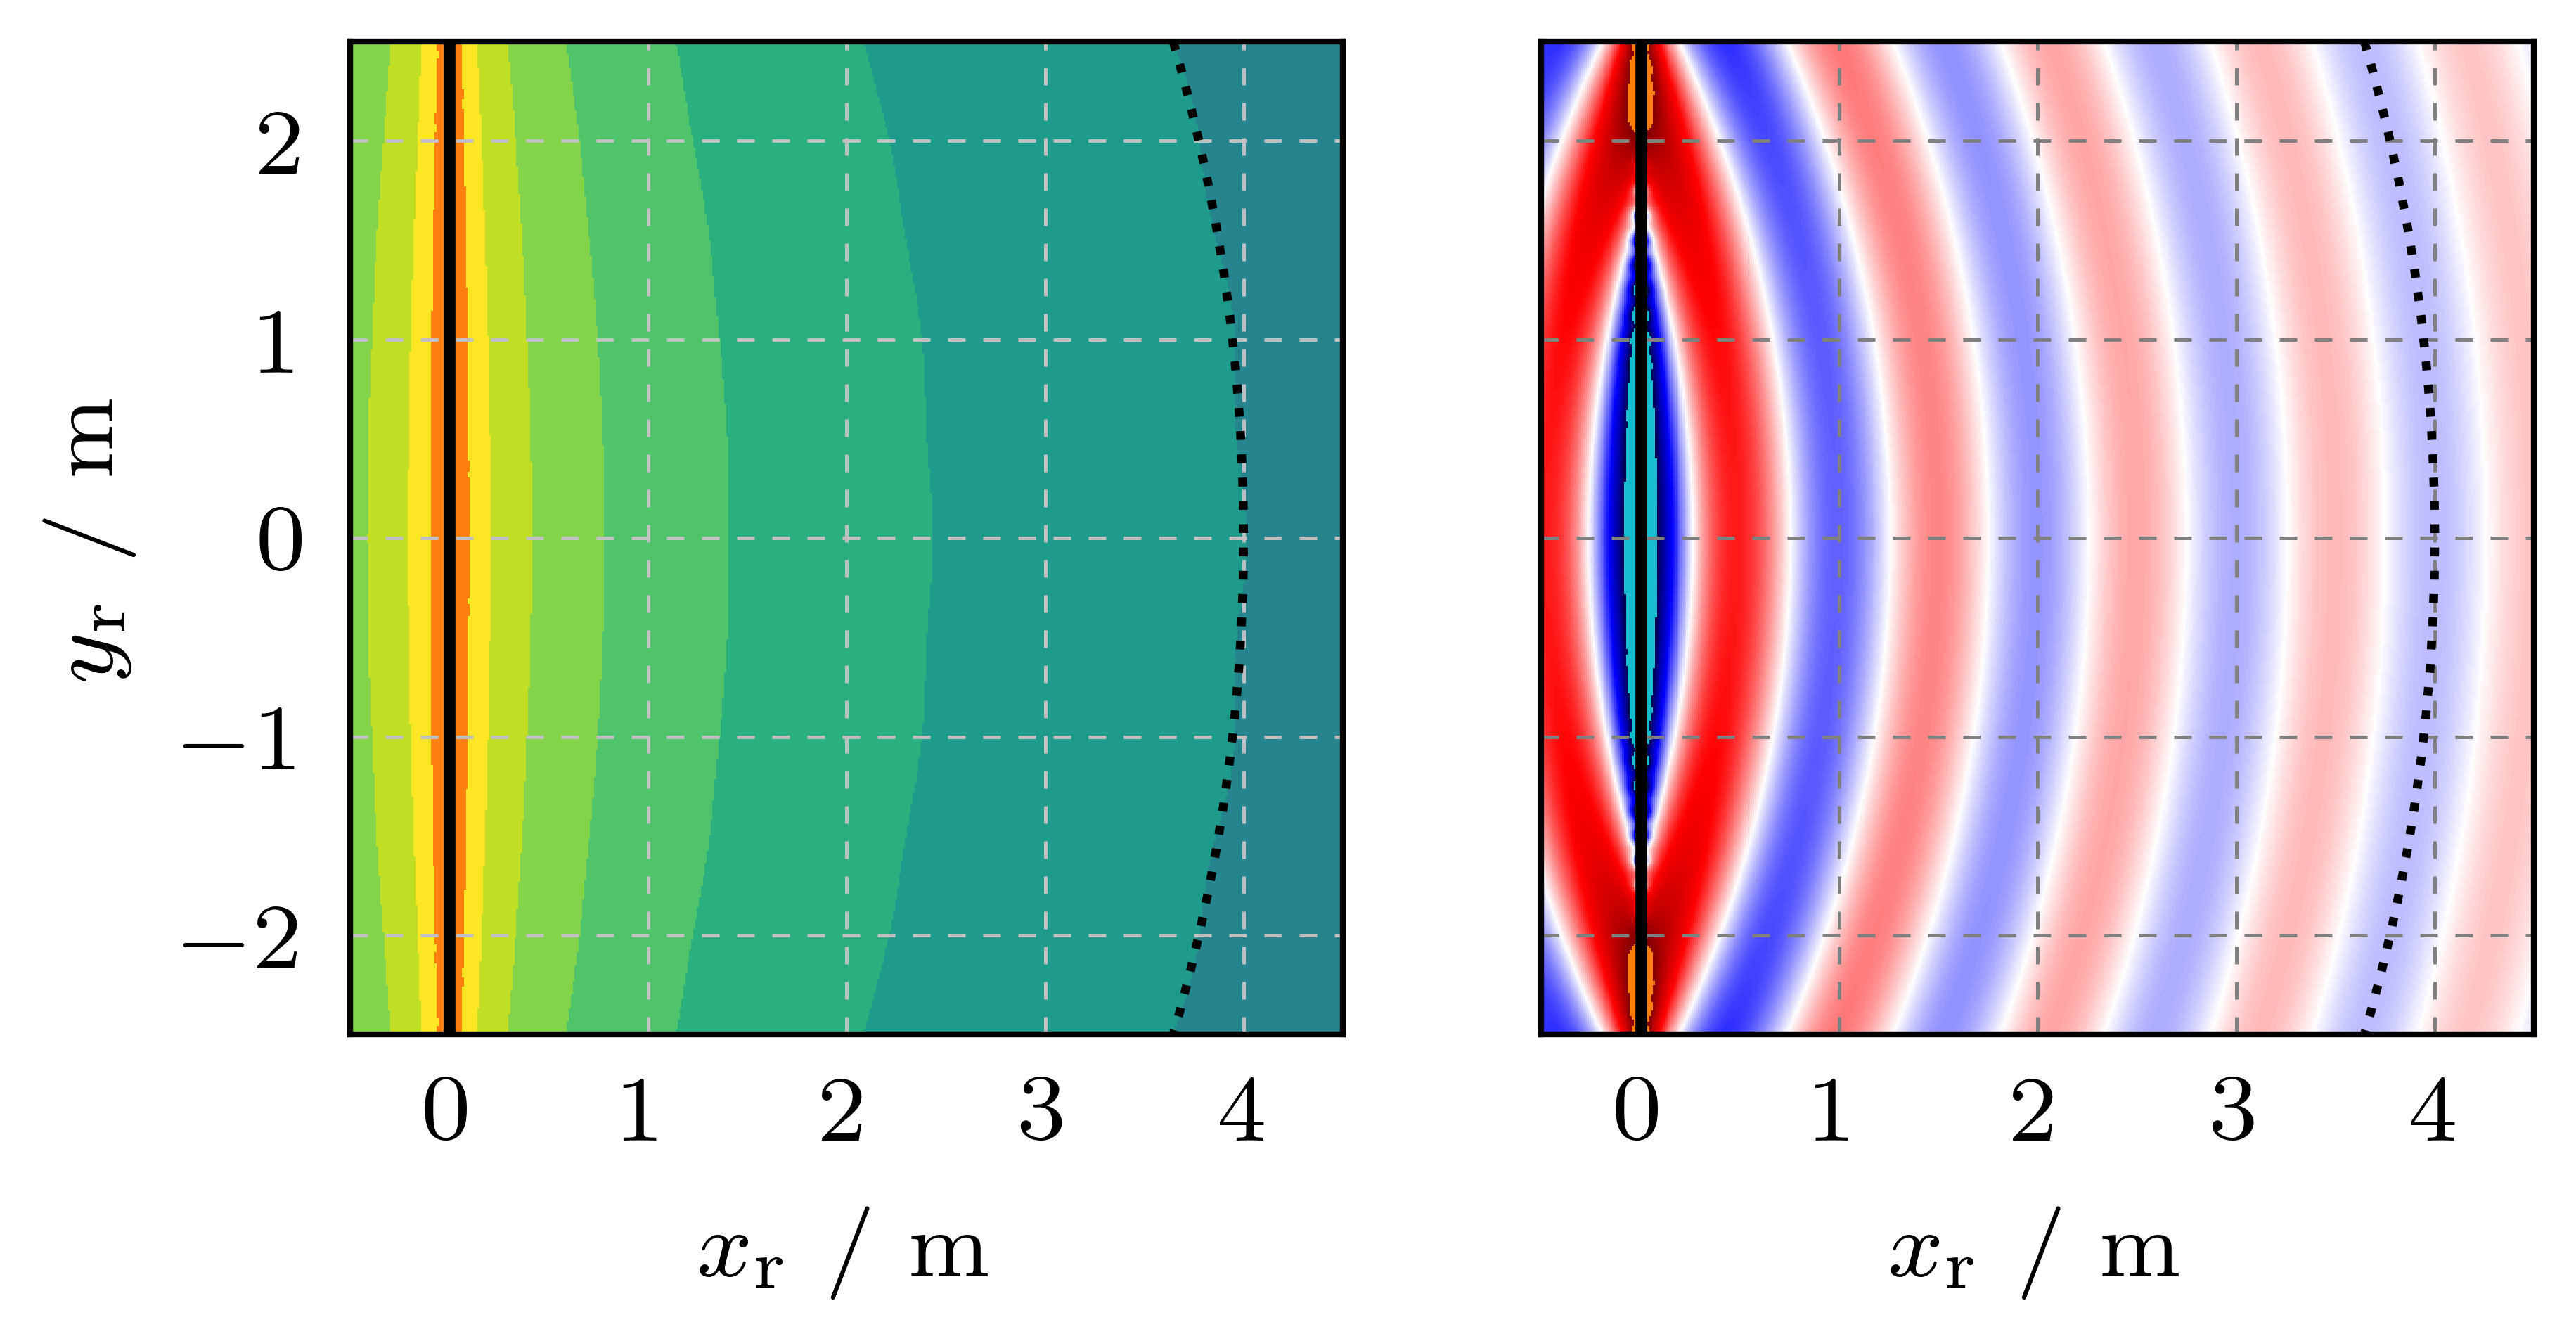
\includegraphics[width=85mm]{../python/wfs25d_lineSSD.png}
\end{plotfigures}
\caption{%2.5D-WFS einer virtuellen Punktquelle bei $\xp = (-5,0,0)^\mathrm{T}$\,m
%mit einem unendlichen Monopol-Array auf der $y$-Achse (schwarz) für
%die Wellenlänge $\lambda=1$\,m.
2.5D WFS of a virtual point source at $\xp = (-5,0,0)^\mathrm{T}$\,m with
the wavelength $\lambda=1$\,m using an infinite, continuous monopole array
on the $y$-axis (black).
%
%Entlang der Referenzkurve -- der gestrichelte, schwarze Kreisbogen -- erfolgt eine
%Amplitudenkorrektur auf Schalldruckamplitude Eins (rechts) bzw. $0$\,dB-Schalldruckpegel (links).
Amplitude correction is applied for the reference curve, i.e. the dotted black
arc.
Along this curve, unit amplitude (right) and $0$\,dB level (left)
results.
%
%Schallfeld mit deutlich erkennbarer Kugel-Wellenfrontkrümmung und gezeigtem
%Zeitbezug für einen Schalldruckwert~$-1$ entlang der Referenzkurve.
The chosen time yields an instantaneous sound pressure value $-1$
along the reference curve.
The sound field exhibits a spherical wavefront curvature.
%
%Farbskalierung wie in \myfig\ref{fig:plot_colorbar}.
Colour scaling according to \myfig\ref{fig:plot_colorbar}.
\cc
}
\label{fig:wfs25d_lineSSD}
\end{figure}



%\subsection{Monofrequentes Schallfeld}
\subsection{Single-Frequency Sound Fields}

%\myfig\ref{fig:wfs25d_lineSSD} zeigt die 2.5D-WFS einer virtuellen Punktquelle
%mit sekundären Monopolquellen infinitesimalen Abstands entlang einer unendlich
%langen Linie auf der $y$-Achse.
\myfig\ref{fig:wfs25d_lineSSD} shows the 2.5D WFS of a virtual point source
using an infinite, linear array on the $y$-axis with secondary monopole sources
at infinitesimal spacing.
%
%Amplitudenkorrekte Synthese ergibt sich entlang des eingezeichneten Kreisbogens,
%der den Punkt $\xr = (4,0,0)^\mathrm{T}$\,m schneidet.
Amplitude-corrected synthesis results along the dotted circular arc,
which intersects the point $\xr = (4,0,0)^\mathrm{T}$\,m.
%
%Die Wellenfrontkrümmung\index{Wellenfrontkrümmung} einer Punktquelle ist ersichtlich.
The wavefront curvature\index{wavefront curvature} of a point source
is evident.
%
%Da für das unendlich lange Array kein Nah-/Fernfeldübergang existiert,
%bleibt die gewünschte Wellenfrontkrümmung der virtuellen Quelle
%über alle Entfernungen erhalten.
Since there is no near-field/far-field transition for the infinite
array, the desired wavefront curvature of a virtual source is
maintained for all distances.
%
%Die für 2.5D-WFS charakteristische Schalldruckamplitudenabnahme
%kann mit \myeq\eqref{eq:pStat25D} quantitativ für ein Punktpaar
%stationärer Phase beschrieben werden.
The decay in sound pressure, which is characteristic of 2.5D WFS, can be
quantitatively described by \eqref{eq:pStat25D}
for a stationary phase point pair.
%
%Wenn Schalldrücke und Pegel jenseits der pegelrichtigen Referenzkurve von
%Interesse sind, muss diese nichtlineare Funktion bezüglich $\xs$, $\xr$ und
%der Primärquellenposition
%$\xp$ (welche die Wellenfrontkrümmung beeinflusst) analysiert
%werden, vgl. \cite{Sonke2000_diss,Wittek2007_diss, Spors2010a}.
This non-linear function can also be used for the analysis of the sound
pressure at the stationary phase positions off the amplitude-corrected
reference curve in relation to $\xs$, $\xr$ and the position of
the virtual source $\xp$,
cf. \cite{Sonke2000_diss,Wittek2007_diss,Spors2010a}.
%
%Dies ist in der 2.5D-WFS-Praxis (bzw. allgemeingültig für alle
%2.5D-Schallfeldsyntheseverfahren) vor allem dann relevant, wenn mehrere virtuelle
%Quellen gleichzeitig und näherungsweise pegelrichtig für einen größeren
%Zuhörerbereich synthetisiert werden sollen.
While it generally applies to all 2.5D sound field synthesis methods,
this analysis is particularly relevant for 2.5D WFS when synthesising
multiple virtual sources with proper mixing balance for a larger listening area.



% please DO NOT rescale the figure and keep it single column
\begin{figure}
\centering
\begin{plotfigures}
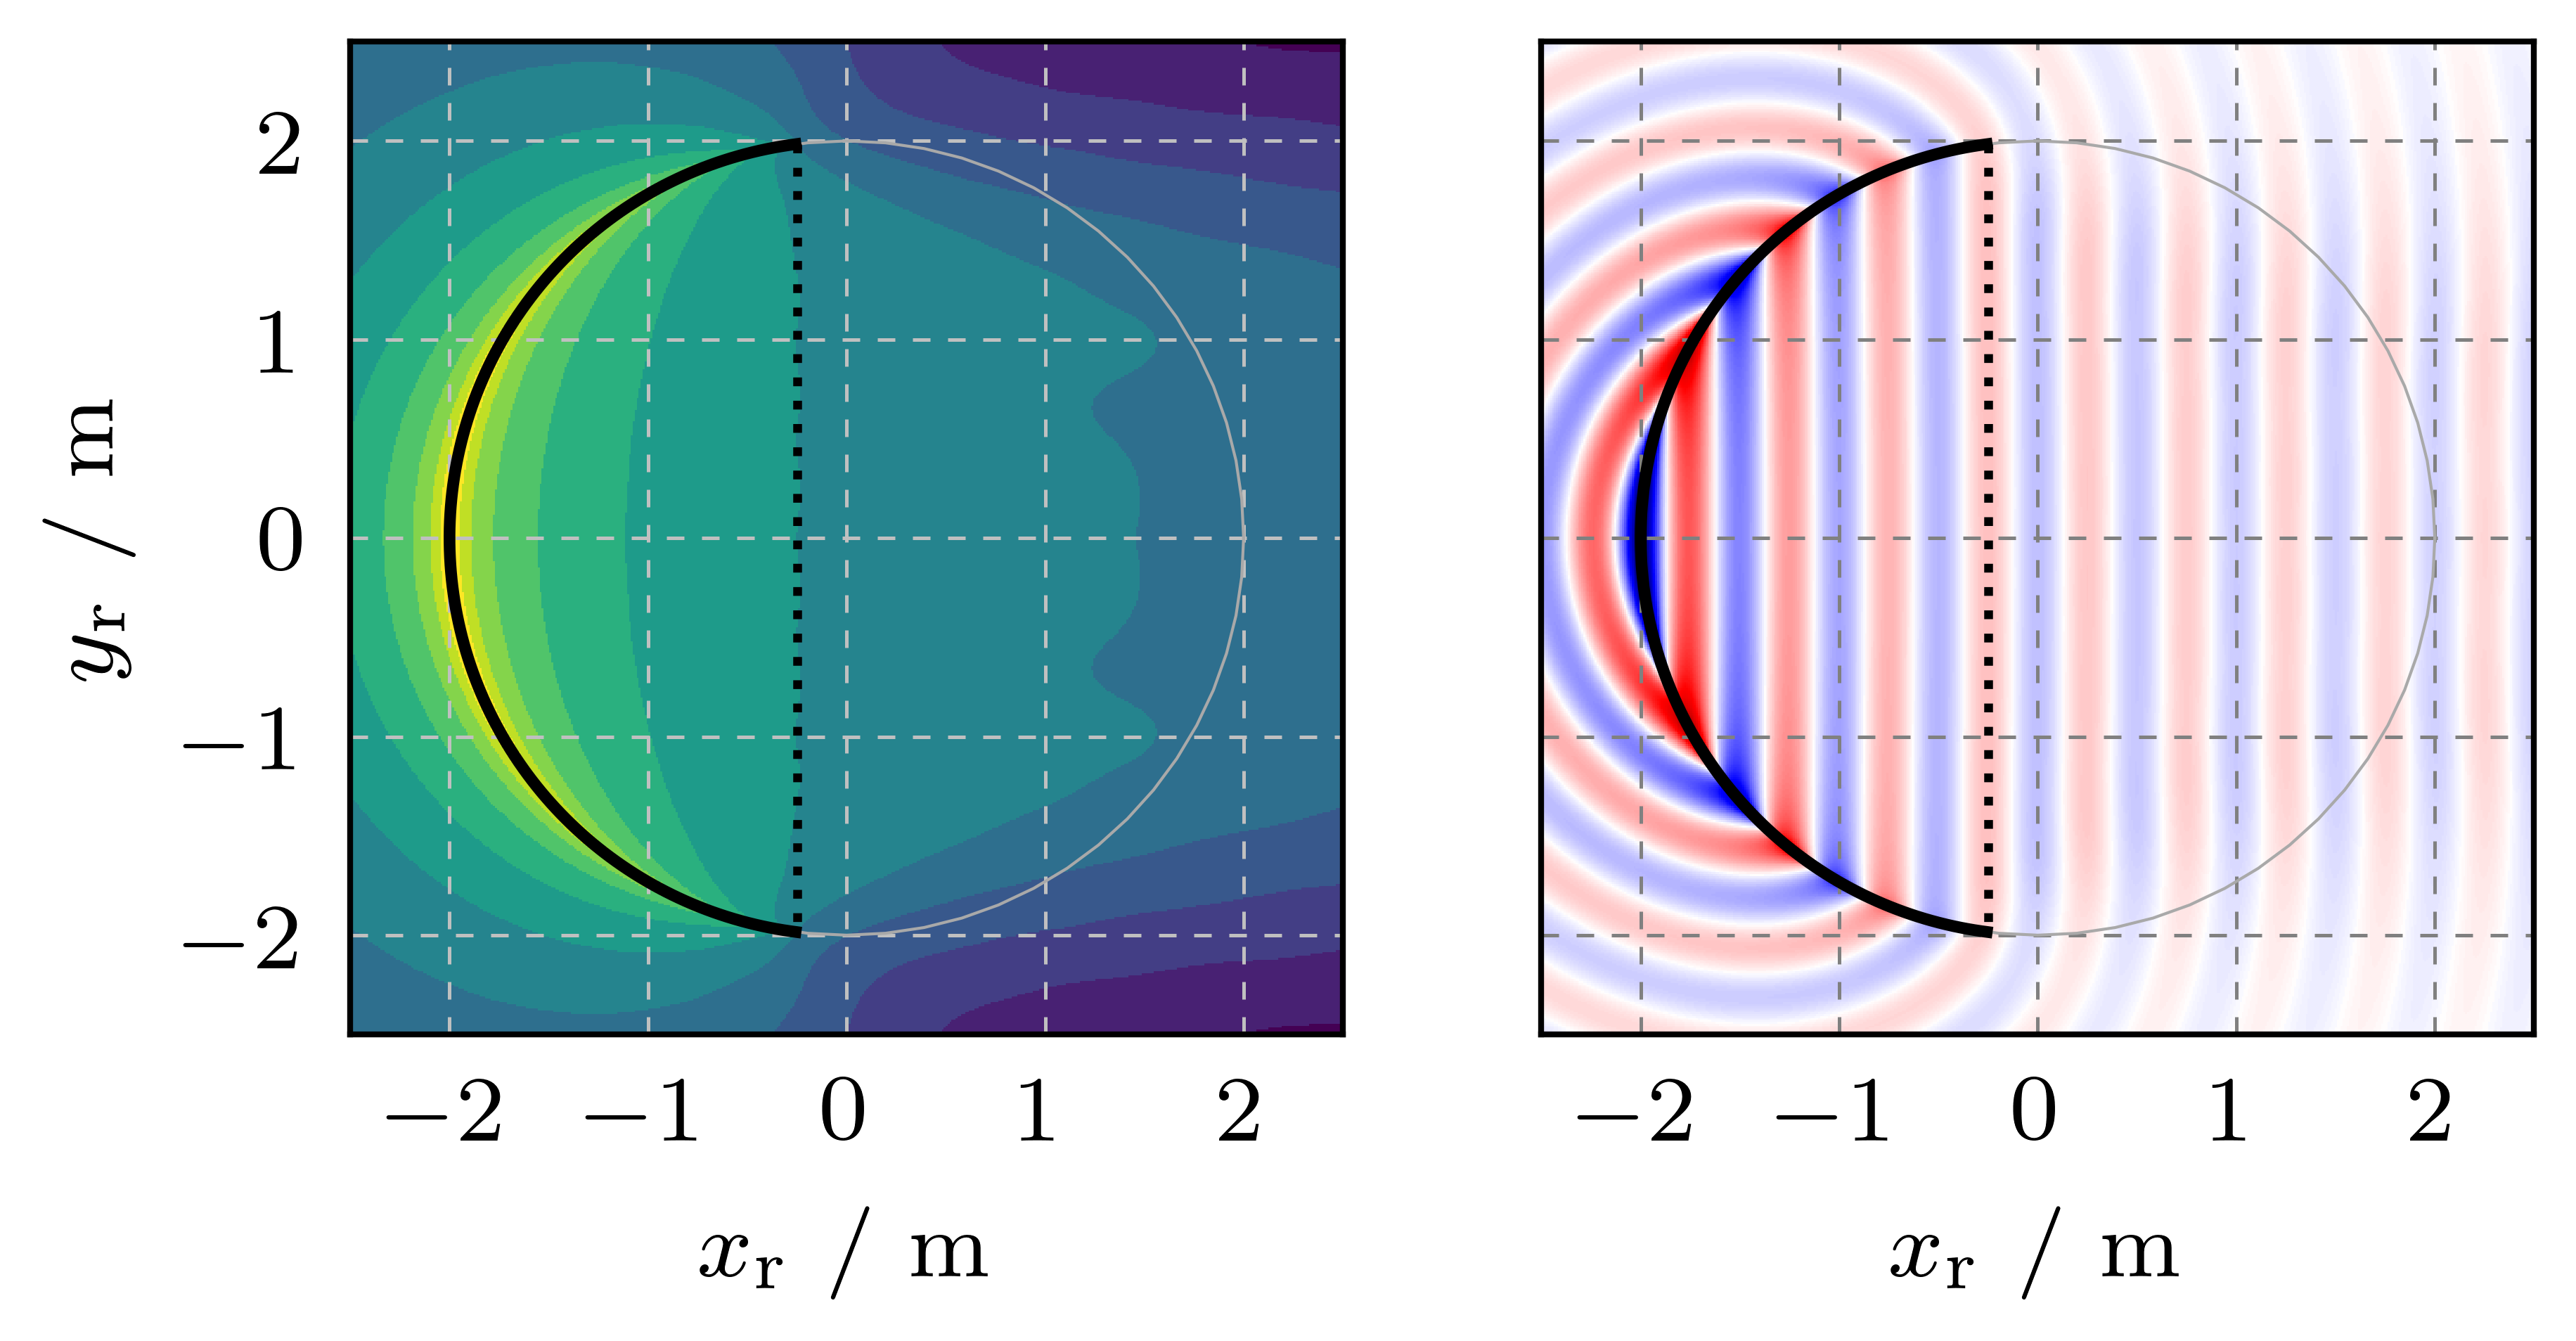
\includegraphics[width=85mm]{../python/wfs25d_circSSD.png}
\end{plotfigures}
\caption{%2.5D-WFS einer virtuellen Punktquelle bei $\xp = (-100,0,0)^\mathrm{T}$\,m
%mit einem 2\,m-Radius-Kreisarray (aktiv beitragende Monopole in schwarz, vgl.~\eqref{eq:SecSrcSel})
%für die Wellenlänge $\lambda=\frac{1}{2}$\,m.
2.5D WFS of a virtual point source at $\xp = (-100,0,0)^\mathrm{T}$\,m with the
wavelength $\lambda=\frac{1}{2}$\,m using a continuous, circular monopole
array with a radius of 2 m.
Active monopoles according to the secondary source selection \eqref{eq:SecSrcSel}
drawn in black.
%
%Entlang der Referenzkurve -- hier die gestrichelte schwarze Linie bei
%$x=-\frac{1}{4}$\,m -- erfolgt
%eine Amplitudenkorrektur auf Schalldruckamplitude Eins bzw. $0$\,dB-Schalldruckpegel.
%
Amplitude correction is applied for the reference curve, i.e. the dotted vertical
line at $x=-\frac{1}{4}$\,m.
Along this line, unit amplitude (right) and $0$\,dB level (left) results.
%
%Schallfeld, mit im Zuhörerbereich verschwindender Wellenfrontkrümmung, visualisiert
%für einen Zeitpunkt bei dem Schalldruckwert~$+1$ entlang der Referenzlinie vorliegt.
The chosen time yields an instantaneous sound pressure value $+1$
along the reference line.
The sound field exhibits a quasi-planar wavefront in the vicinity of the array.
%
\cc
}
\label{fig:wfs25d_circSSD}
\end{figure}



%In \myfig\ref{fig:wfs25d_circSSD} wird ein kreisförmiges,
%kontinuierliches Monopol-Array benutzt.
In \myfig\ref{fig:wfs25d_circSSD}, a circular, continuous monopole array is used.
%
%
%2.5D-WFS einer ebenen Wellenfront -- also eine Welle
%mit verschwindender Wellenfrontkrümmung innerhalb der Zuhörerfläche -- wurde
%mit einer sehr weit entfernten virtuellen Punktquelle angenähert.
A distant virtual point source produces a negligible wavefront curvature
within the listening area.
This is employed for the 2.5D WFS of a planar wavefront.
%
%Amplitudenkorrekte Synthese erfolgt für \myfig\ref{fig:wfs25d_circSSD}
%auf der Linie bei $x=-\frac{1}{4}$\,m.
The amplitude-corrected synthesis for \myfig\ref{fig:wfs25d_circSSD}
occurs along the vertical line at $x=-\frac{1}{4}$\,m.
%
%Für alle anderen Empfängerpunkte gilt wieder die in 2.5D-WFS
%charakteristische Schalldruckamplitudenabnahme im Nahfeld des Arrays.
For all other probe points in the near field of the array, the 2.5D
characteristic decay applies to the sound pressure over distance.
%
%Im frequenzabhängigen Fernfeld des Arrays geht die ebene Wellenfrontkrümmung
%(virtuelle Quelle) in die einer Punktquelle (Lautsprecherarray) über,
%einhergehend mit $6$\,dB-Pegelverlust pro Entfernungsverdopplung.
In the frequency-dependent far field of the array, the curvature of the planar
wavefront (i.e. the characteristic of the virtual source)
changes to that of a point source (i.e. the characteristic of the
physical loudspeaker array), accompanied by a $6$\,dB level loss per
doubling of distance.



% please DO NOT rescale the figure and keep it single column
\begin{figure}
\centering
\begin{plotfigures}
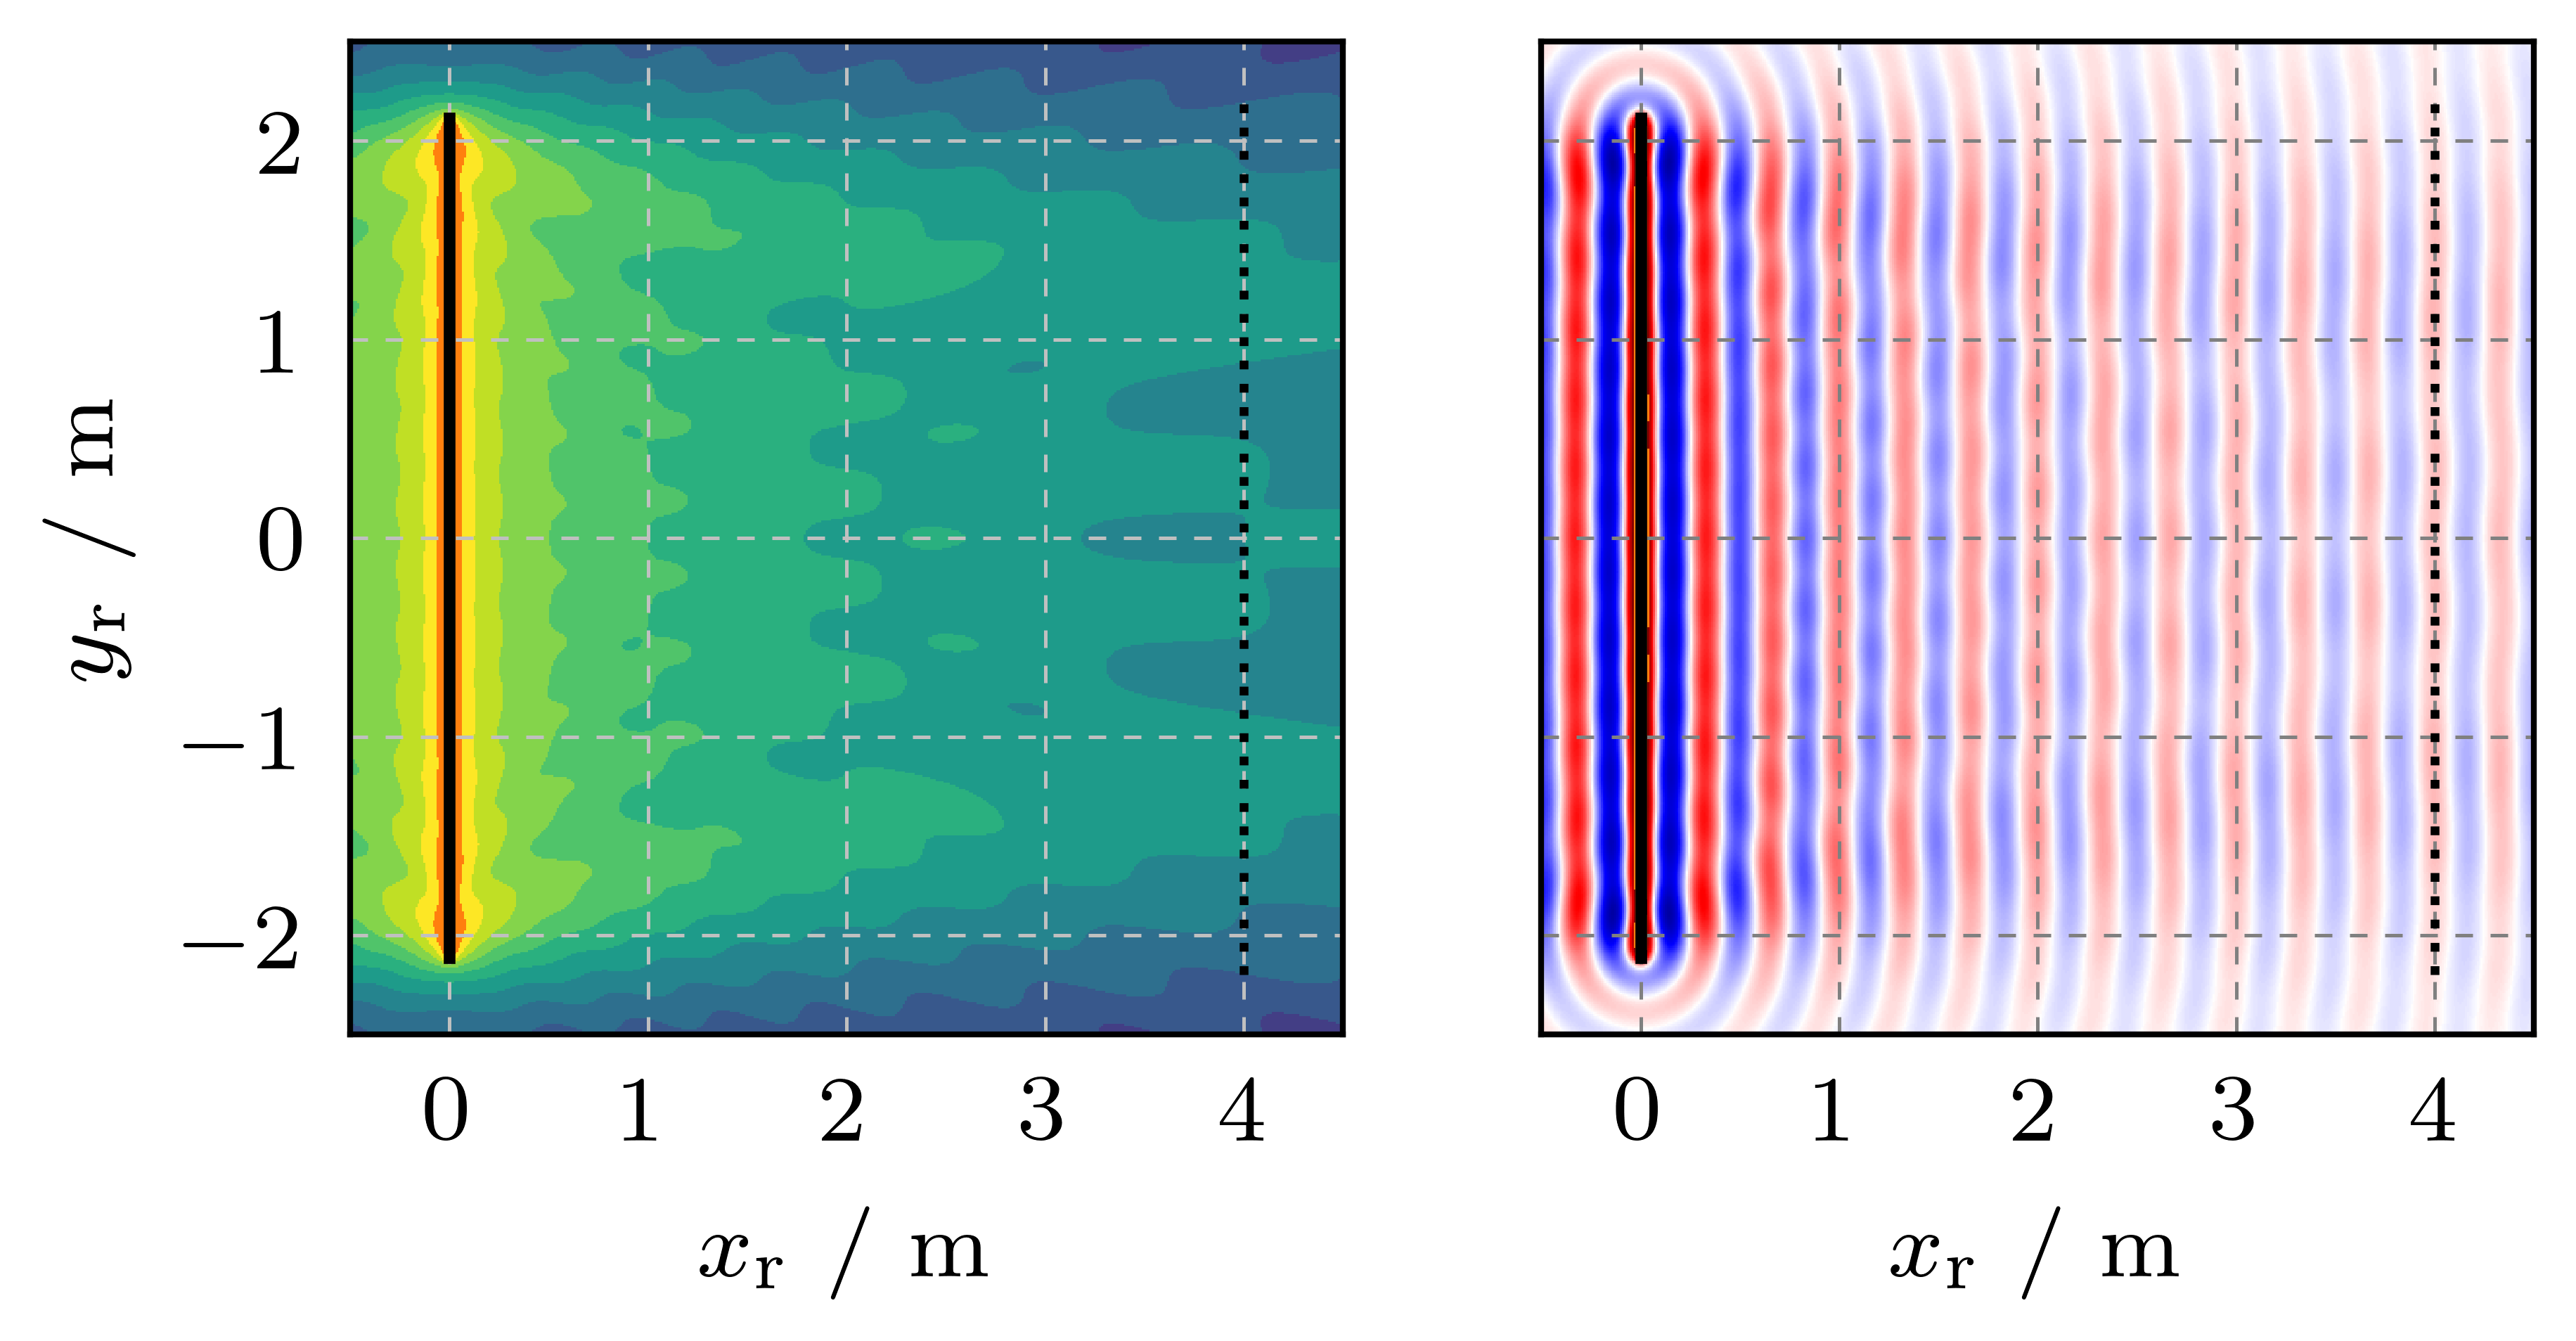
\includegraphics[width=85mm]{../python/wfs25d_lineSSD_truncation.png}
\end{plotfigures}
\caption{%2.5D-WFS einer virtuellen Punktquelle bei
%$\xp = (-100,0,0)^\mathrm{T}$\,m mit endlichem, kontinuierlichen Monopol-Array
%entlang der $y$-Achse für die Wellenlänge $\lambda=\frac{1}{3}$\,m.
2.5D WFS of a virtual point source at $\xp = (-100,0,0)^\mathrm{T}$\,m with
the wavelength $\lambda=\frac{1}{3}$\,m using a finite-length, continuous
monopole array on the $y$-axis (black).
%
%Amplitudenkorrektur auf $0$\,dB-Pegel entlang der schwarz-gestrichelten
%Referenzlinie bei $x=4$\,m.
Amplitude correction towards $0$\,dB level is applied for the reference
line at $x=4$\,m (dotted black line).
%
%Beugung an einem endlichem Array:
Diffraction artefacts due to the finite-length array can be observed:
%Wellen mit anderen Laufrichtungen beeinträchtigen die
%gewünschte ebene Wellenfront im Nahfeld des Arrays. Im Fernfeld des Arrays
%bildet sich die linke Richtcharakteristik in
%\myfig\ref{fig:wfs25d_lineSSD_polar_plot_overlay} aus.
In the near field of the array, waves with different
propagation directions interfere with the desired $0^\circ$-planar
wavefront.
In the far field, the directivity shown in
\myfig\ref{fig:wfs25d_lineSSD_polar_plot_overlay}~(left) applies.
%
\cc
}
\label{fig:wfs25d_lineSSD_truncation}
\end{figure}



% please DO NOT rescale the figure and keep it single column
\begin{figure}
\centering
\begin{plotfigures}
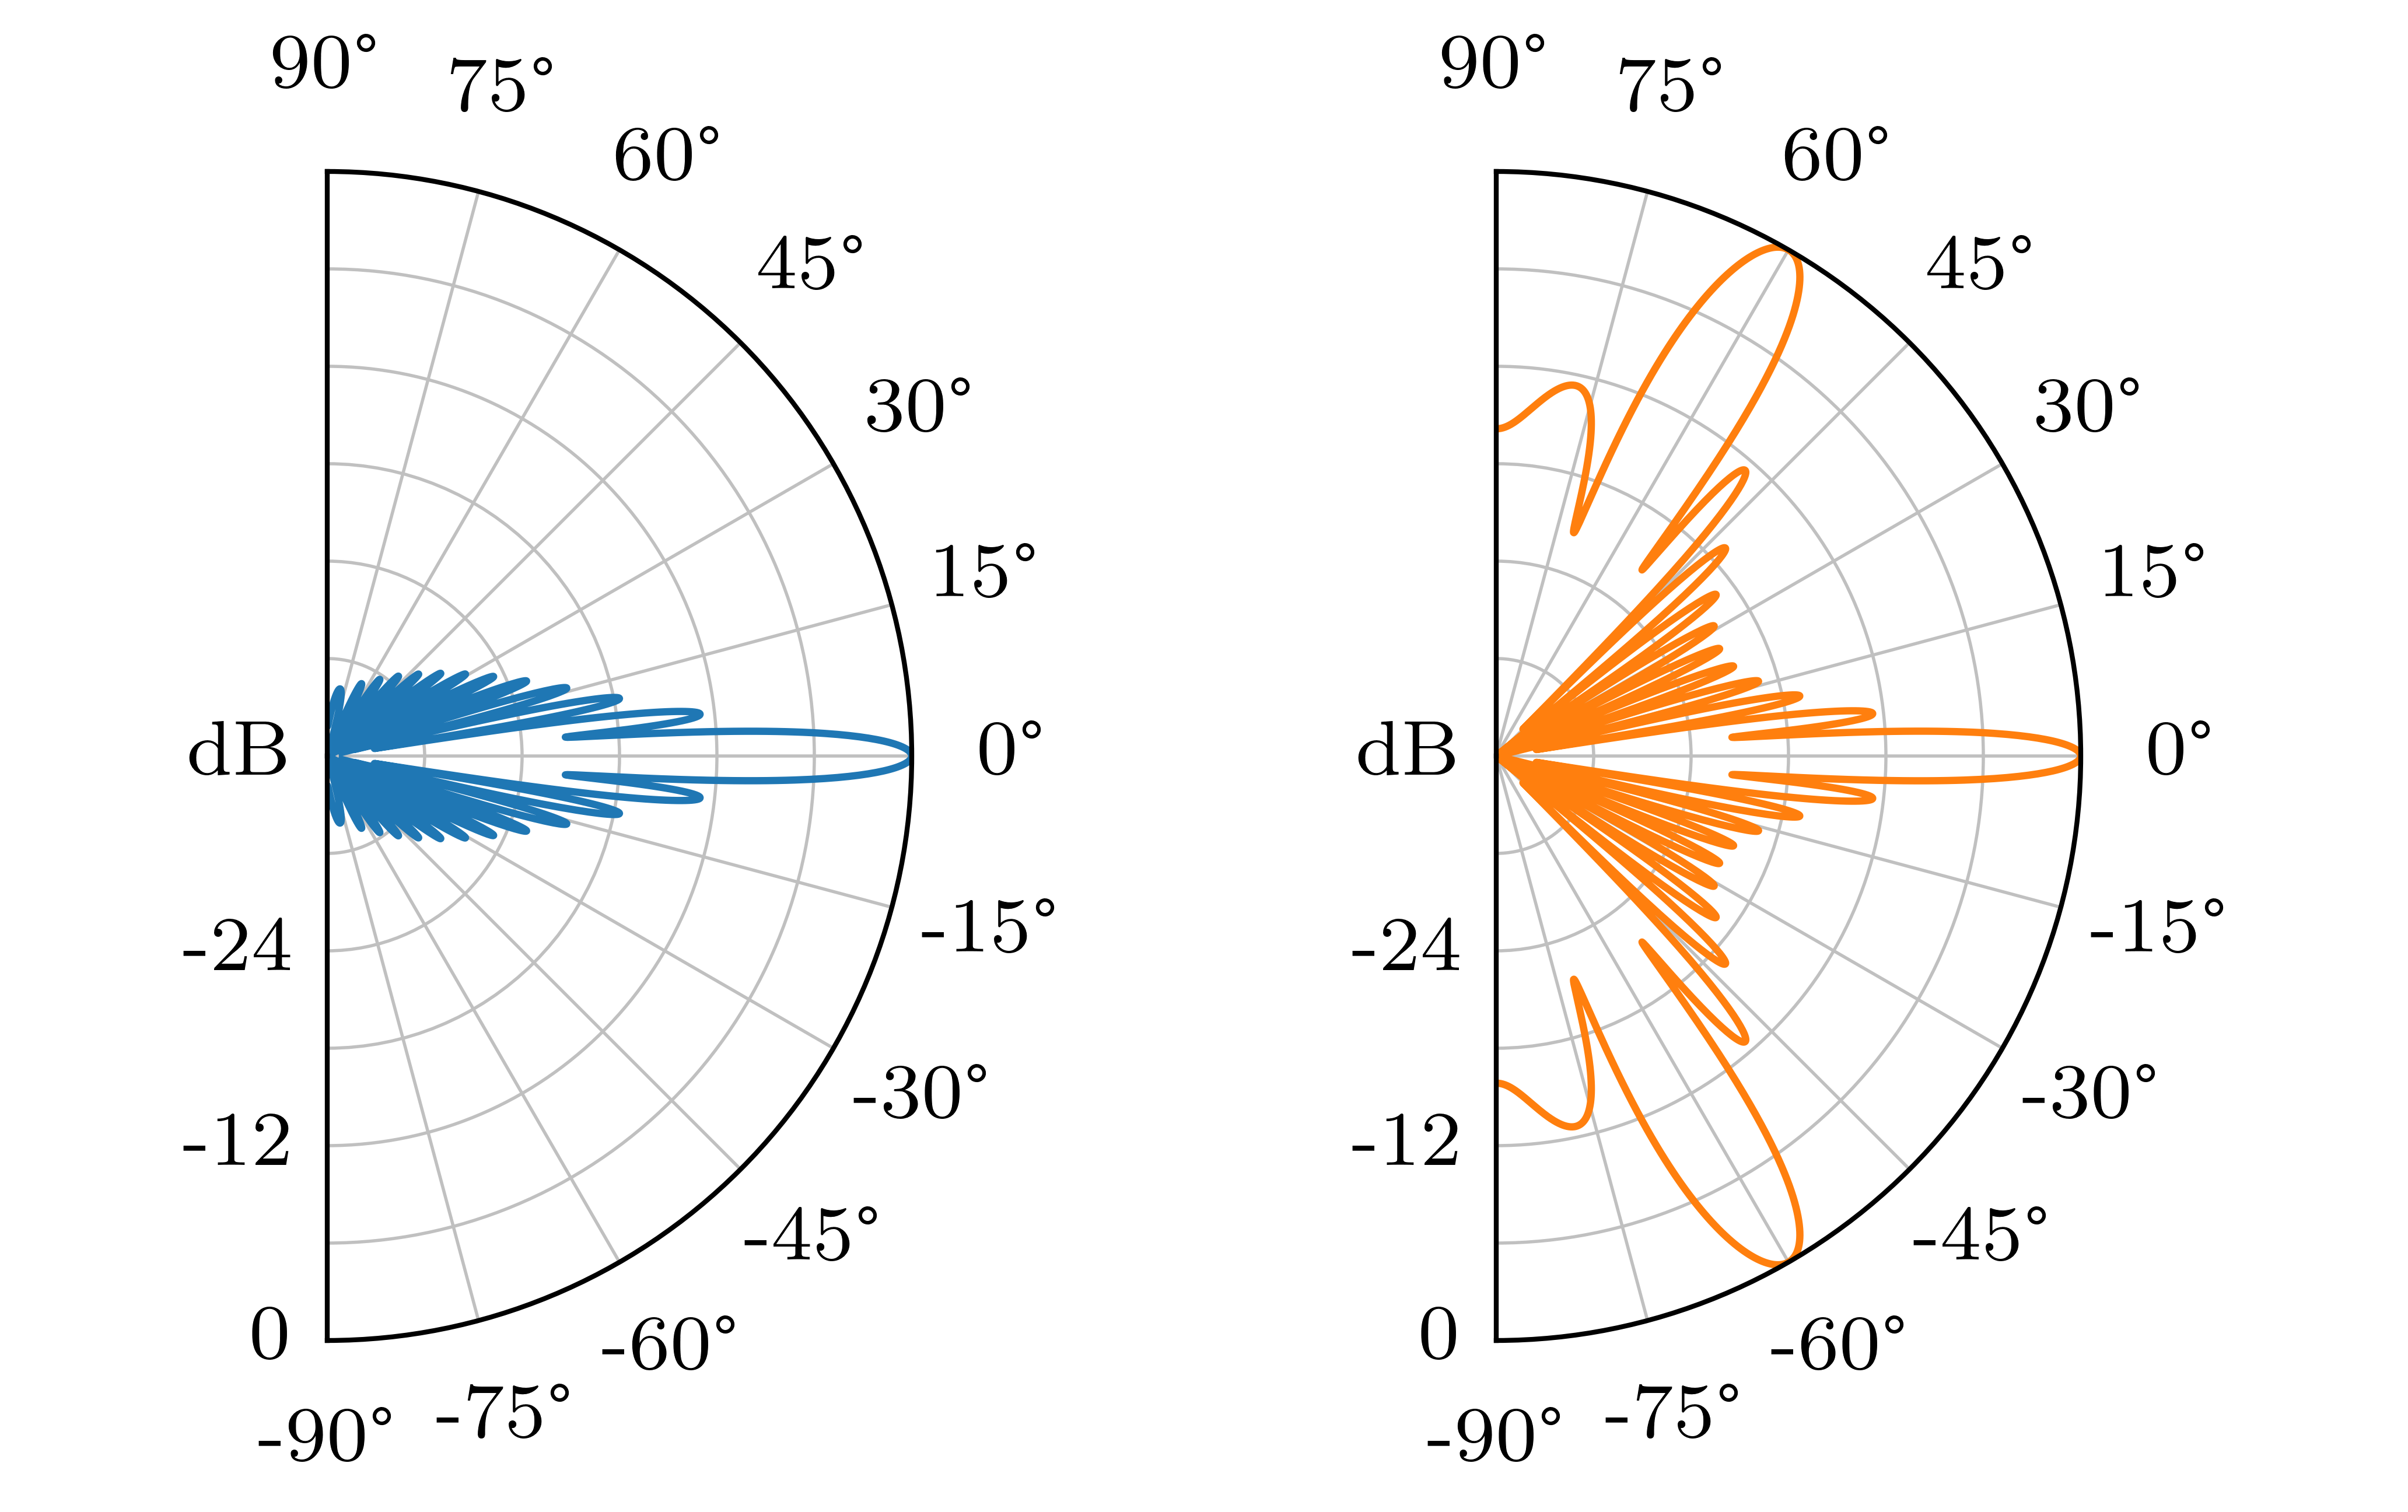
\includegraphics[width=85mm]{../python/wfs25d_lineSSD_polar_plot_overlay.png}
\end{plotfigures}
\caption{
%Fernfeldrichtcharakteristiken für
%Wellenlänge $\lambda=\frac{1}{3}$\,m, $\frac{2\pi}{\lambda} L \approx 79{,}807$
%und gleicher virtueller Primärquelle, aber
%verschiedene Sekundärquellenverteilungen.
Far-field directivities for
$\lambda=\frac{1}{3}$\,m, $\frac{2\pi}{\lambda} L \approx 79{.}807$\,rad
of the same primary source (a distant virtual point source), but for two
different secondary source distributions (finite-length,
linear monopole array).
%
%Links, blau für \myfig\ref{fig:wfs25d_lineSSD_truncation} und
%rechts, orange für \myfig\ref{fig:wfs25d_lineSSD_aliasing}.
The blue directivity on the left is related
to \myfig\ref{fig:wfs25d_lineSSD_truncation}
and the orange directivity on the right corresponds
to \myfig\ref{fig:wfs25d_lineSSD_aliasing}.
%
%Das Szenario aus \myfig\ref{fig:wfs25d_lineSSD_truncation} erzeugt im Fernfeld
%eine $0^\circ$-Hauptkeule\index{Hauptkeule}
%(\textit{main lobe}\index{main lobe})
%und viele Nebenkeulen\index{Nebenkeule}
%(\textit{side lobes}\index{side lobe}).
The \myfig\ref{fig:wfs25d_lineSSD_truncation} shows a scenario
that yields a main lobe\index{main lobe} at $0^\circ$
and numerous side lobes\index{side lobe} in the far-field directivity.
%
%Das Szenario aus \myfig\ref{fig:wfs25d_lineSSD_aliasing} erzeugt im Fernfeld zusätzlich
%zur $0^\circ$-Hauptkeule für die gewählte Wellenlänge zwei etwas breitere
%Gitterkeulen\index{Gitterkeule} (\textit{grating lobes}\index{grating lobe})
%bei exakt $\pm 60^\circ$ mit gleichem Pegel, sowie viele Nebenkeulen.
%
The \myfig\ref{fig:wfs25d_lineSSD_aliasing} shows a scenario
that yields a main lobe at $0^\circ$, two additional, slightly broader
so called grating lobes\index{grating lobe} at (intentionally) exactly
$\pm 60^\circ$ with the same level,
as well as numerous side lobes in the far-field directivity.
%
%Gitterkeulen stehen in Verbindung zu räumlichem Aliasing, Nebenkeulen zu Beugung.
Grating lobes are related to spatial aliasing\index{spatial aliasing},
side lobes are related to diffraction.
%
The direction of these lobes depends on the frequency.  % added in ENG version
%
\cc
}
\label{fig:wfs25d_lineSSD_polar_plot_overlay}
\end{figure}



%In \myfig\ref{fig:wfs25d_lineSSD_truncation} ist die 2.5D-WFS einer ebenen
%Wellenfront mit einem linearen, auf der $y$-Achse liegenden, endlichen
%Monopol-Array visualisiert.
\myfig\ref{fig:wfs25d_lineSSD_truncation} shows the 2.5D WFS of a planar
wavefront using a linear, finite monopole array on the $y$-axis.
%
%Die ebene Wellenfront weist wegen frequenzabhängiger Beugung Artefakte auf.
The planar wavefront exhibits artefacts due to (frequency-dependent)
diffraction.
%
%Diese lassen sich anschaulich mit der in
%\myfig\ref{fig:wfs25d_lineSSD_polar_plot_overlay}~(links)
%dargestellten Fernfeldrichtcharakteristik der gewählten Frequenz erklären.
These can be illustratively explained by means of the (frequency-dependent)
far-field directivity shown in
\myfig\ref{fig:wfs25d_lineSSD_polar_plot_overlay}~(left).
%
%Nebenkeulen korrespondieren mit Wellenfronten im Nahfeld, welche die im
%Polardiagramm indizierten -- im Vergleich zur $0^\circ$-Hauptrichtung der ebenen
%Wellenfront -- anderen Abstrahlrichtungen  aufweisen.
Side lobes in the far field are related to additional wavefronts in
the near field.
Their propagation directions can be deduced from the polar diagram.
These directions apparently differ from the direction of the main lobe,
i.e. the $0^\circ$-direction of the planar wavefront.
%
%Die Wellenfronten interferieren und erzeugen so die Beugungsartefakte.
The wavefronts interfere, which causes diffraction artefacts.
%
%Die Pegel der Nebenkeulen und damit die Beugungsartefakte lassen sich durch
%sogenanntes \textit{tapering} bzw. \textit{gain shading},
%vgl. \cite{Vogel1993_diss,Start1997_diss}, verringern.
The levels of the side lobes can be reduced, and thus the diffraction
artefacts can be modified by means of so called `tapering' or
`gain shading' the driving function,
cf. \cite{Vogel1993_diss,Start1997_diss}.
%
%Dies geht jedoch immer zu Kosten einer breiteren Hauptkeule
%im Fernfeld (vgl. kompromissbehaftetes Fensterdesign in der Signalverarbeitung,
%\cite[Kap.~3.5]{Moeser2009_book}, \cite{Trees2002_book}) und wirkt sich
%daher im Nahfeld auch auf die gewünschte $0^\circ$-Wellenfront aus.
However, this always comes at the expense of a broader main lobe
in the far field (cf. window design compromise in signal processing
\cite[Ch.~3.5]{Moeser2009_book}, \cite[Ch.~3]{Trees2002_book}), and
inherently affects the near field of the desired $0^\circ$-wavefront.



% please DO NOT rescale the figure and keep it single column
\begin{figure}
\centering
\begin{plotfigures}
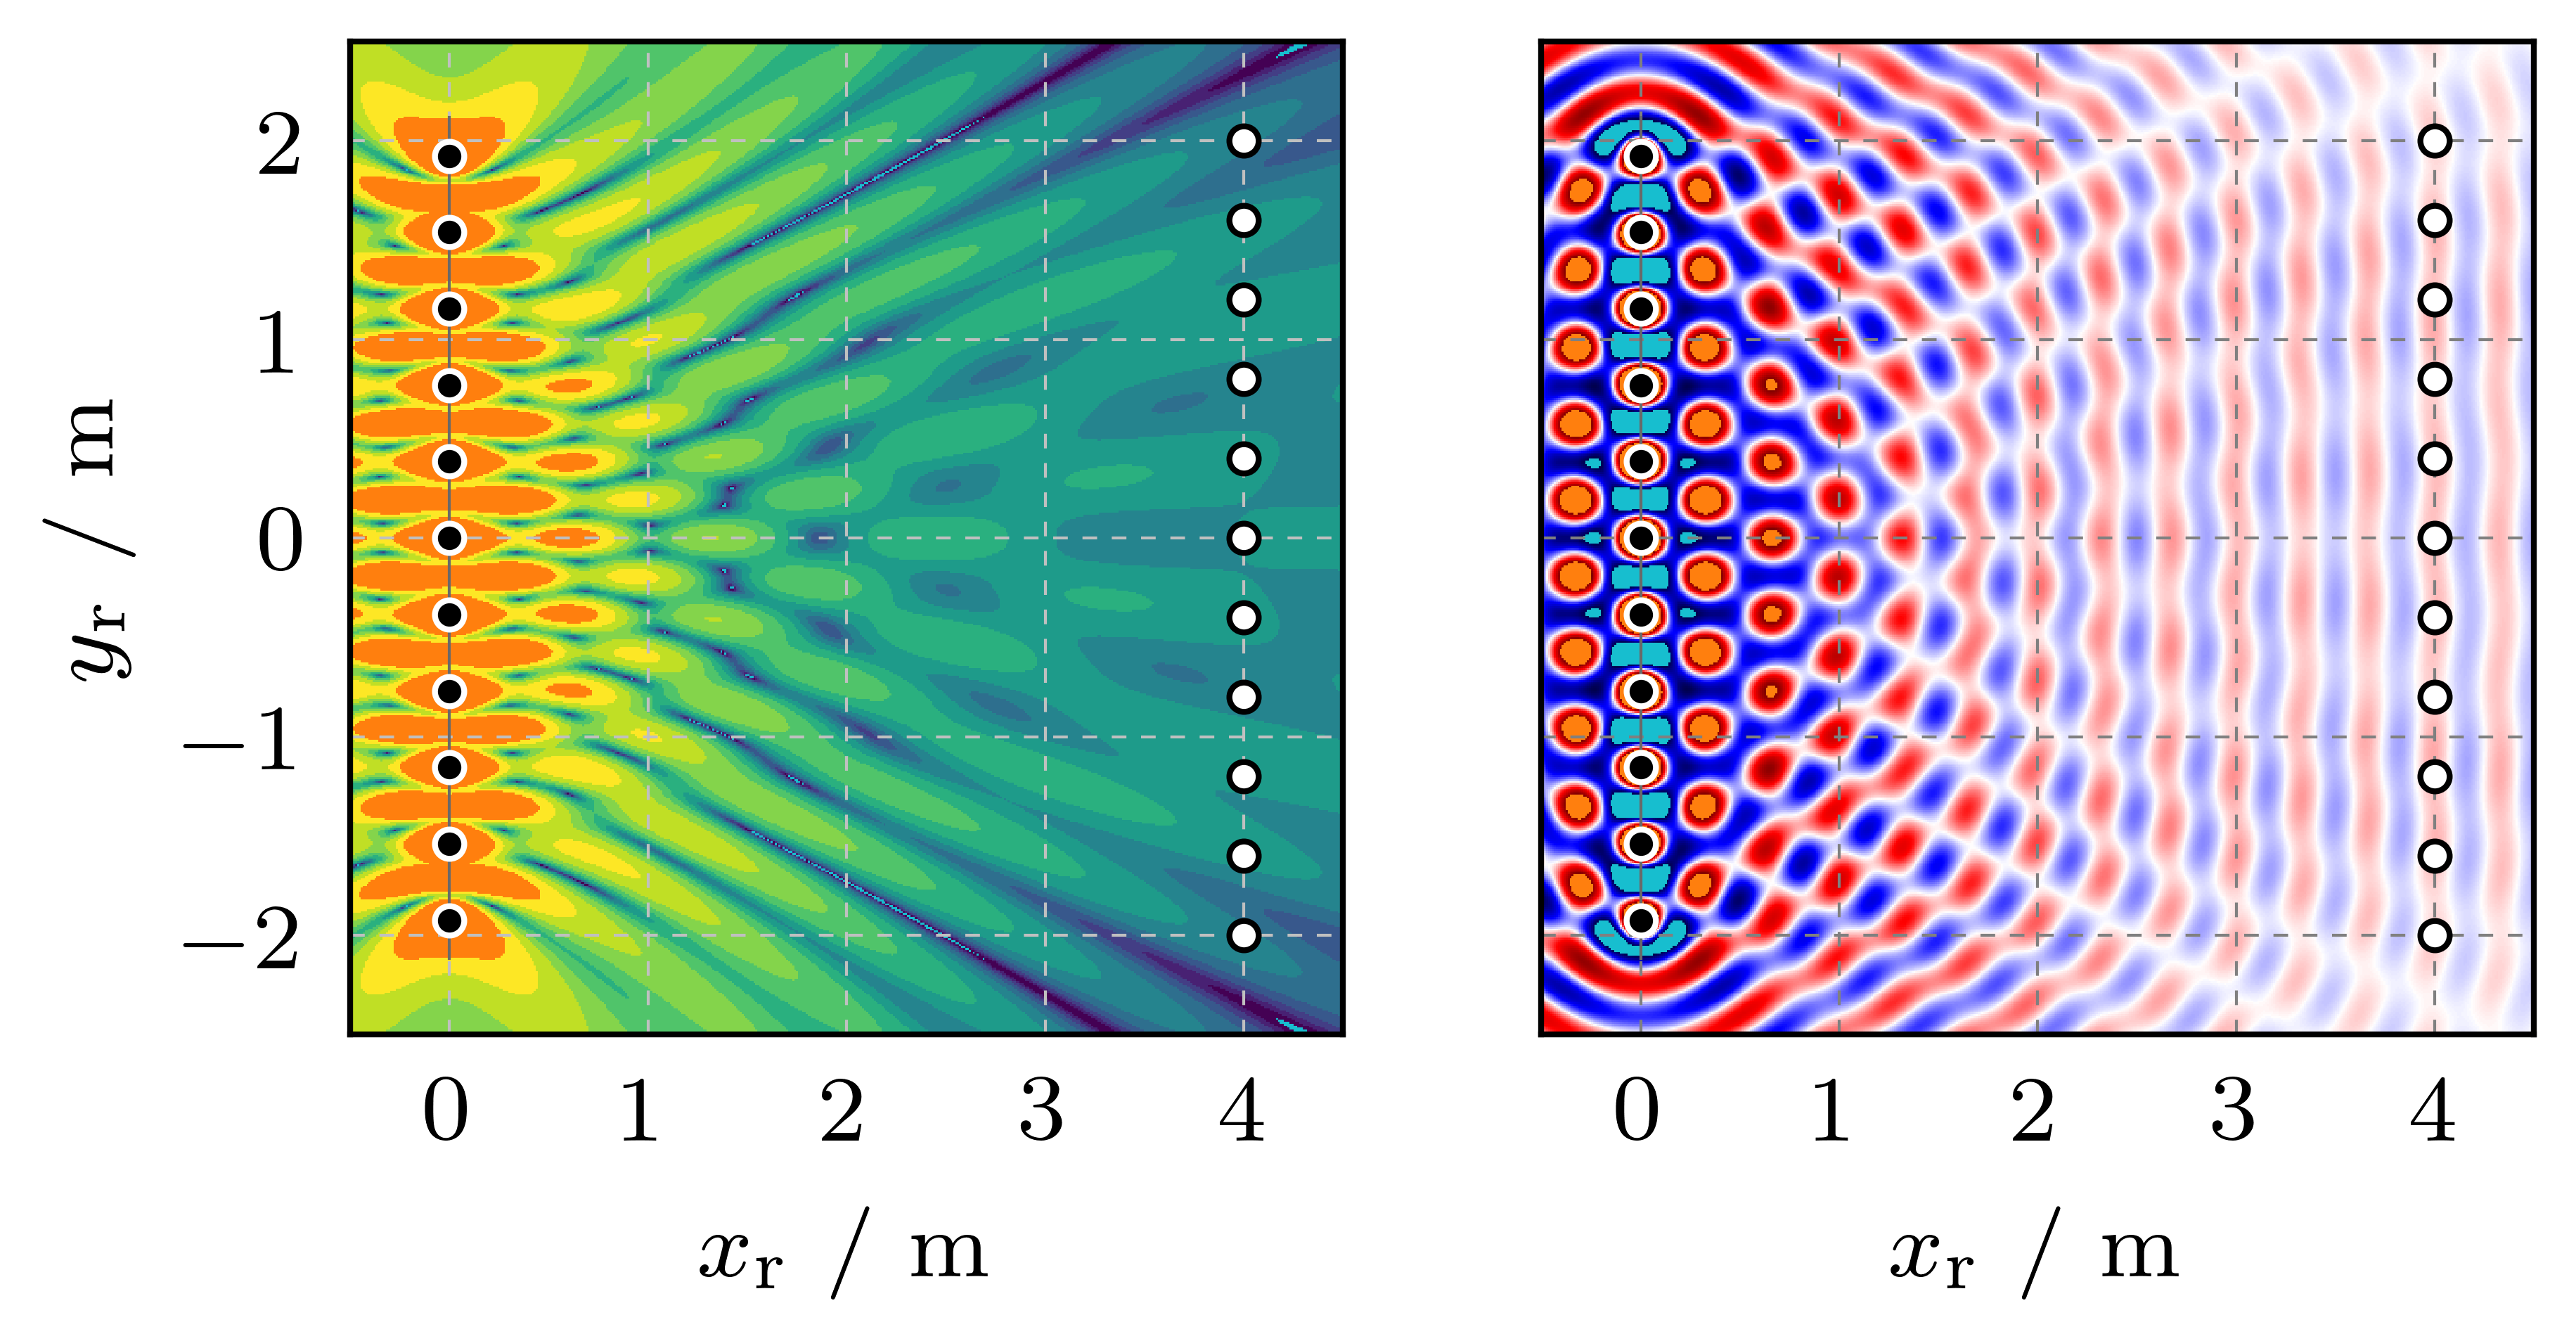
\includegraphics[width=85mm]{../python/wfs25d_lineSSD_aliasing.png}
\end{plotfigures}
\caption{%2.5D-WFS einer virtuellen Punktquelle bei
%$\xp = (-100,0,0)^\mathrm{T}$\,m mit 11 Monopolen entlang der $y$-Achse
%(schwarze Punkte, Abstand $\Delta_{\xs}\approx 0{,}3849$\,m)
%für die Wellenlänge $\lambda=\frac{1}{3}$\,m.
2.5D WFS of a virtual point source $\xp = (-100,0,0)^\mathrm{T}$\,m with
the wavelength $\lambda=\frac{1}{3}$\,m using a finite-length,
discretised monopole array on the $y$-axis (11 monopoles shown with black dots,
equidistant spacing $\Delta_{\xs}\approx 0{.}3849$\,m).
%
%2.5D-WFS-Amplitudenkorrektur auf $0$\,dB-Pegel entlang der Referenzlinie bei
%$x=4$\,m.
Amplitude correction towards $0$\,dB is applied for the reference
line at $x=4$\,m.
%
%Die 11 weißen Punkte auf dieser bilden mit den 11 Monopolen jeweils ein
%Punktpaar mit stationärer Phasenbedingung.
Each of the eleven white dots along the reference line is
related to one monopole.
This establishes eleven pairs of points for a stationary phase condition.
%
%Zusätzlich zur Beugung tritt räumliches Aliasing wegen zu großem Lautsprecherabstand
%$\Delta_{\xs} $ auf:
In addition to diffraction, spatial aliasing occurs because the loudspeaker
distance $\Delta_{\xs}$ is too large for the selected frequency.
%
%vor allem die Wellenanteile mit hohem Pegel und
%Ausbreitungsrichtungen um $\pm 60^\circ$ beeinträchtigen die
%gewünschte ebene $0^\circ$-Wellenfront im Nahfeld des Arrays.
In particular, the wave components with propagation directions around
$\pm 60^\circ$ and high levels heavily affect the desired $0^\circ$-planar
wavefront in the near field of the array.
%
%Im Fernfeld des Arrays bildet sich die Richtcharakteristik
%\myfig\ref{fig:wfs25d_lineSSD_polar_plot_overlay}~(rechts) aus.
In the far field, the directivity shown in
\myfig\ref{fig:wfs25d_lineSSD_polar_plot_overlay}~(right) applies.
%
\cc
}
\label{fig:wfs25d_lineSSD_aliasing}
\end{figure}



%In \myfig\ref{fig:wfs25d_lineSSD_aliasing} ist die 2.5D-WFS einer ebenen Wellenfront
%mit einem endlichen, linearen Monopol-Array entlang der $y$-Achse visualisiert.
In \myfig\ref{fig:wfs25d_lineSSD_aliasing}, the 2.5D WFS of a planar wavefront
with a linear, finite monopole array along the $y$-axis is visualised.
%
%Die Arraylänge $L \approx 4{,}234$\,m und die Wellenlänge $\lambda=\frac{1}{3}$\,m sind
%gleich gewählt wie bei \myfig\ref{fig:wfs25d_lineSSD_truncation}.
The array length $L \approx 4{.}234$ m and the wavelength
$\lambda=\frac{1}{3}$ m are chosen to be the same as
in \myfig\ref{fig:wfs25d_lineSSD_truncation}.
%
%Nun aber weisen die sekundären Monopole einen Abstand von
%$\Delta_{\xs}\approx 0{,}3849$\,m auf; das Array ist räumlich diskretisiert.
However, the array is spatially discretised here: The secondary monopoles
are arranged at a distance of $\Delta_{\xs}\approx 0{.}3849$\,m.
%
%Für dieses Szenario treten neben Beugungsartefakten zusätzlich
%frequenzabhängige Artefakte auf, welche auf den endlichen Abstand der
%Sekundärquellen zurückzuführen sind.
In addition to diffraction, frequency-dependent artefacts occur in this
scenario due to the finite distance between the secondary sources.
%
%Diese Artefakte sind bekannt als räumliches Aliasing und beeinträchtigen die
%gewünschte Wellenfront deutlich ausgeprägter als Beugung.
These artefacts are referred to as spatial aliasing\index{spatial aliasing}
and have a much greater impact on the desired wavefront than diffraction.



%Gemäß des räumlichen Abtastkriteriums\index{Abtastkriterium, räumlich},
%vgl. \cite[Kap.~26.4]{Skudrzyk1971}, wird räumliches Aliasing\index{Aliasing, räumlich}
%in der Wellenfront vollständig vermieden, wenn für die höchste im Ansteuerungssignal
%vorkommende Frequenz $f_\text{max}$ der hüllkonturspezifische Abstand
%$\Delta_{\xs}$
%\begin{align}
%\label{eq:SamplingCriterion}
%\Delta_{\xs} < \frac{c}{2 f_\text{max}}\quad\leftrightarrow\quad
%\Delta_{\xs} < \frac{\lambda_\text{min}}{2}
%\end{align}
%zwischen zwei Lautsprechern eingehalten wird, vgl. \cite[S.~246]{Stenzel1927},
%\cite[Kap.~4]{Winter2019_diss}.
According to the spatial sampling criterion\index{spatial sampling criterion},
cf. \cite[Ch.~26.4]{Skudrzyk1971}, spatial aliasing does not occur
under the condition \cite[p.~246]{Stenzel1927}
%, \cite[Ch.~4]{Winter2019_diss} omit Fiete's thesis in favour of
%strengthening Stenzel's innovation for acoustics and
%Skudrzyk's classical textbook
\begin{align}
\label{eq:SamplingCriterion}
\Delta_{\xs} < \frac{c}{2 f_\text{max}}\quad\leftrightarrow\quad
\Delta_{\xs} < \frac{\lambda_\text{min}}{2},
\end{align}
where $f_\text{max}$ denotes the maximum occurring frequency
(and $\lambda_\text{min}$ the minimum occurring wavelength)
in the audio signal, and $\Delta_{\xs}$ the contour-specific distance
between adjacent loudspeakers.
%
%Im Falle eines linearen Arrays entspricht $\Delta_{\xs}$ direkt dem
%Lautsprecherabstand.
In the case of a uniform linear array, $\Delta_{\xs}$
directly corresponds to the loudspeaker spacing.
%
%Für konvexe Arrays gilt dieses harte Kriterium als sehr gute Näherung;
%im Fall des dichtbepackten Kreisarrays kann die Kreisbogenlänge zwischen
%zwei benachbarten Lautsprechern für $\Delta_{\xs}$ verwendet werden.
For convex arrays, this strict criterion is considered a very good
approximation; in the case of a densely packed circular array,
the arc length between two adjacent loudspeakers can be used for
$\Delta_{\xs}$.



%Für die oberen 3--4 Oktaven des menschlichen Hörvermögens bedingt
%die \myeq\eqref{eq:SamplingCriterion}
%erheblichen Hardwareaufwand wegen der erforderlichen sehr kleinen
%Lautsprecherabstände.
For the upper three to four octaves of the human hearing range,
\myeq\eqref{eq:SamplingCriterion} necessitates a dense arrangement of
loudspeakers. This requires considerable hardware effort.
%
%Bei praxisnahen WFS-Systemen mit typischen Lautsprecherabständen zwischen
%$0{,}1 \dots 0{,}25\,\text{m}$ tritt räumliches Aliasing bei Frequenzen oberhalb
%$1715 \dots 686\,\text{Hz}$
%auf.
In practical WFS systems with typical loudspeaker distances between
$0{.}1 \dots 0{.}25\,\text{m}$, spatial aliasing occurs at frequencies
above $1715 \dots 686\,\text{Hz}$.
%(calculation for $c=343$\,m/s).



%Im Beispiel von \myfig\ref{fig:wfs25d_lineSSD_aliasing} wird die
%\myeq\eqref{eq:SamplingCriterion}
%wegen
%$\Delta_{\xs}\approx 0{,}3849\,\text{m} > \frac{\lambda}{2}=\frac{1}{6}\,\text{m}$
%verletzt.
In the example in \myfig\ref{fig:wfs25d_lineSSD_aliasing},
\myeq\eqref{eq:SamplingCriterion} is not satisfied because
$\Delta_{\xs}\approx 0{.}3849\,\text{m} > 0{.}1\bar{6}\,\text{m} = \frac{1}{6}\,\text{m} = \frac{\lambda}{2}$.
%
%Artefakte von räumlichem Aliasing entstehen durch Wellenfronten anderer
%Ausbreitungsrichtungen, die mit der gewünschten, hier ebenen $0^\circ$-Wellenfront
%interferieren.
Spatial aliasing artefacts arise when aliasing wavefronts
with different propagation directions interfere with the desired planar
$0^\circ$-wavefront.
%
%Die frequenzabhängige Anzahl und Ausbreitungsrichtung(en) der
%Aliasing-Wellenfronten,
%vgl. \cite{Stenzel1927,Berkhout1993_JASA,Start1997_diss, Winter2019_diss},
%lässt sich u.a. aus der
%Fernfeldrichtcharakteristik in
%\myfig\ref{fig:wfs25d_lineSSD_polar_plot_overlay}~(rechts) bestimmen.
The (frequency-dependent) number and propagation direction(s) of these
additional aliasing wavefronts, cf.
\cite{Stenzel1927,Berkhout1993_JASA,Start1997_diss,Winter2019_diss},
can be determined from the (frequency-dependent) far-field
directivity shown in \myfig\ref{fig:wfs25d_lineSSD_polar_plot_overlay}~(right).
%
%Im Beispiel sind es die beiden sogenannten Gitterkeulen
%bei exakt $\pm 60^\circ$,
%welche bei Benutzung von omnidirektional abstrahlenden
%Monopol-Sekundärquellen
%den gleichen Pegel wie die $0^\circ$-Hauptkeule
%aufweisen.
In this example, two so called grating lobes\index{grating lobe}
occur at exactly $\varphi=\pm 60^\circ$, due to the relation
$\frac{2\pi}{\Delta_{\xs}} = \frac{\omega}{c} \sin(|\varphi|)$,
cf. \cite[Ch.~2.4]{Trees2002_book}.
As secondary monopole sources exhibit no spatial filtering characteristics,
grating lobes have the same level as the desired $0^\circ$ main lobe.



%Das Schallfeld ist im Nahfeld erst in einiger Entfernung zum endlichen Array
%näherungsweise aliasing-frei, im Beispiel gilt das bei der gewählten Frequenz
%grob jenseits der Referenzlinie bei $x=4$\,m mittig vor dem Array.
The sound field becomes approximately aliasing-free
at a certain distance for the chosen example.
For the selected frequency, this applies roughly at the midpoint of the
array behind the reference line at $x=4$\,m.



% please DO NOT rescale the figure and keep it single column
\begin{figure}
\centering
\begin{plotfigures}
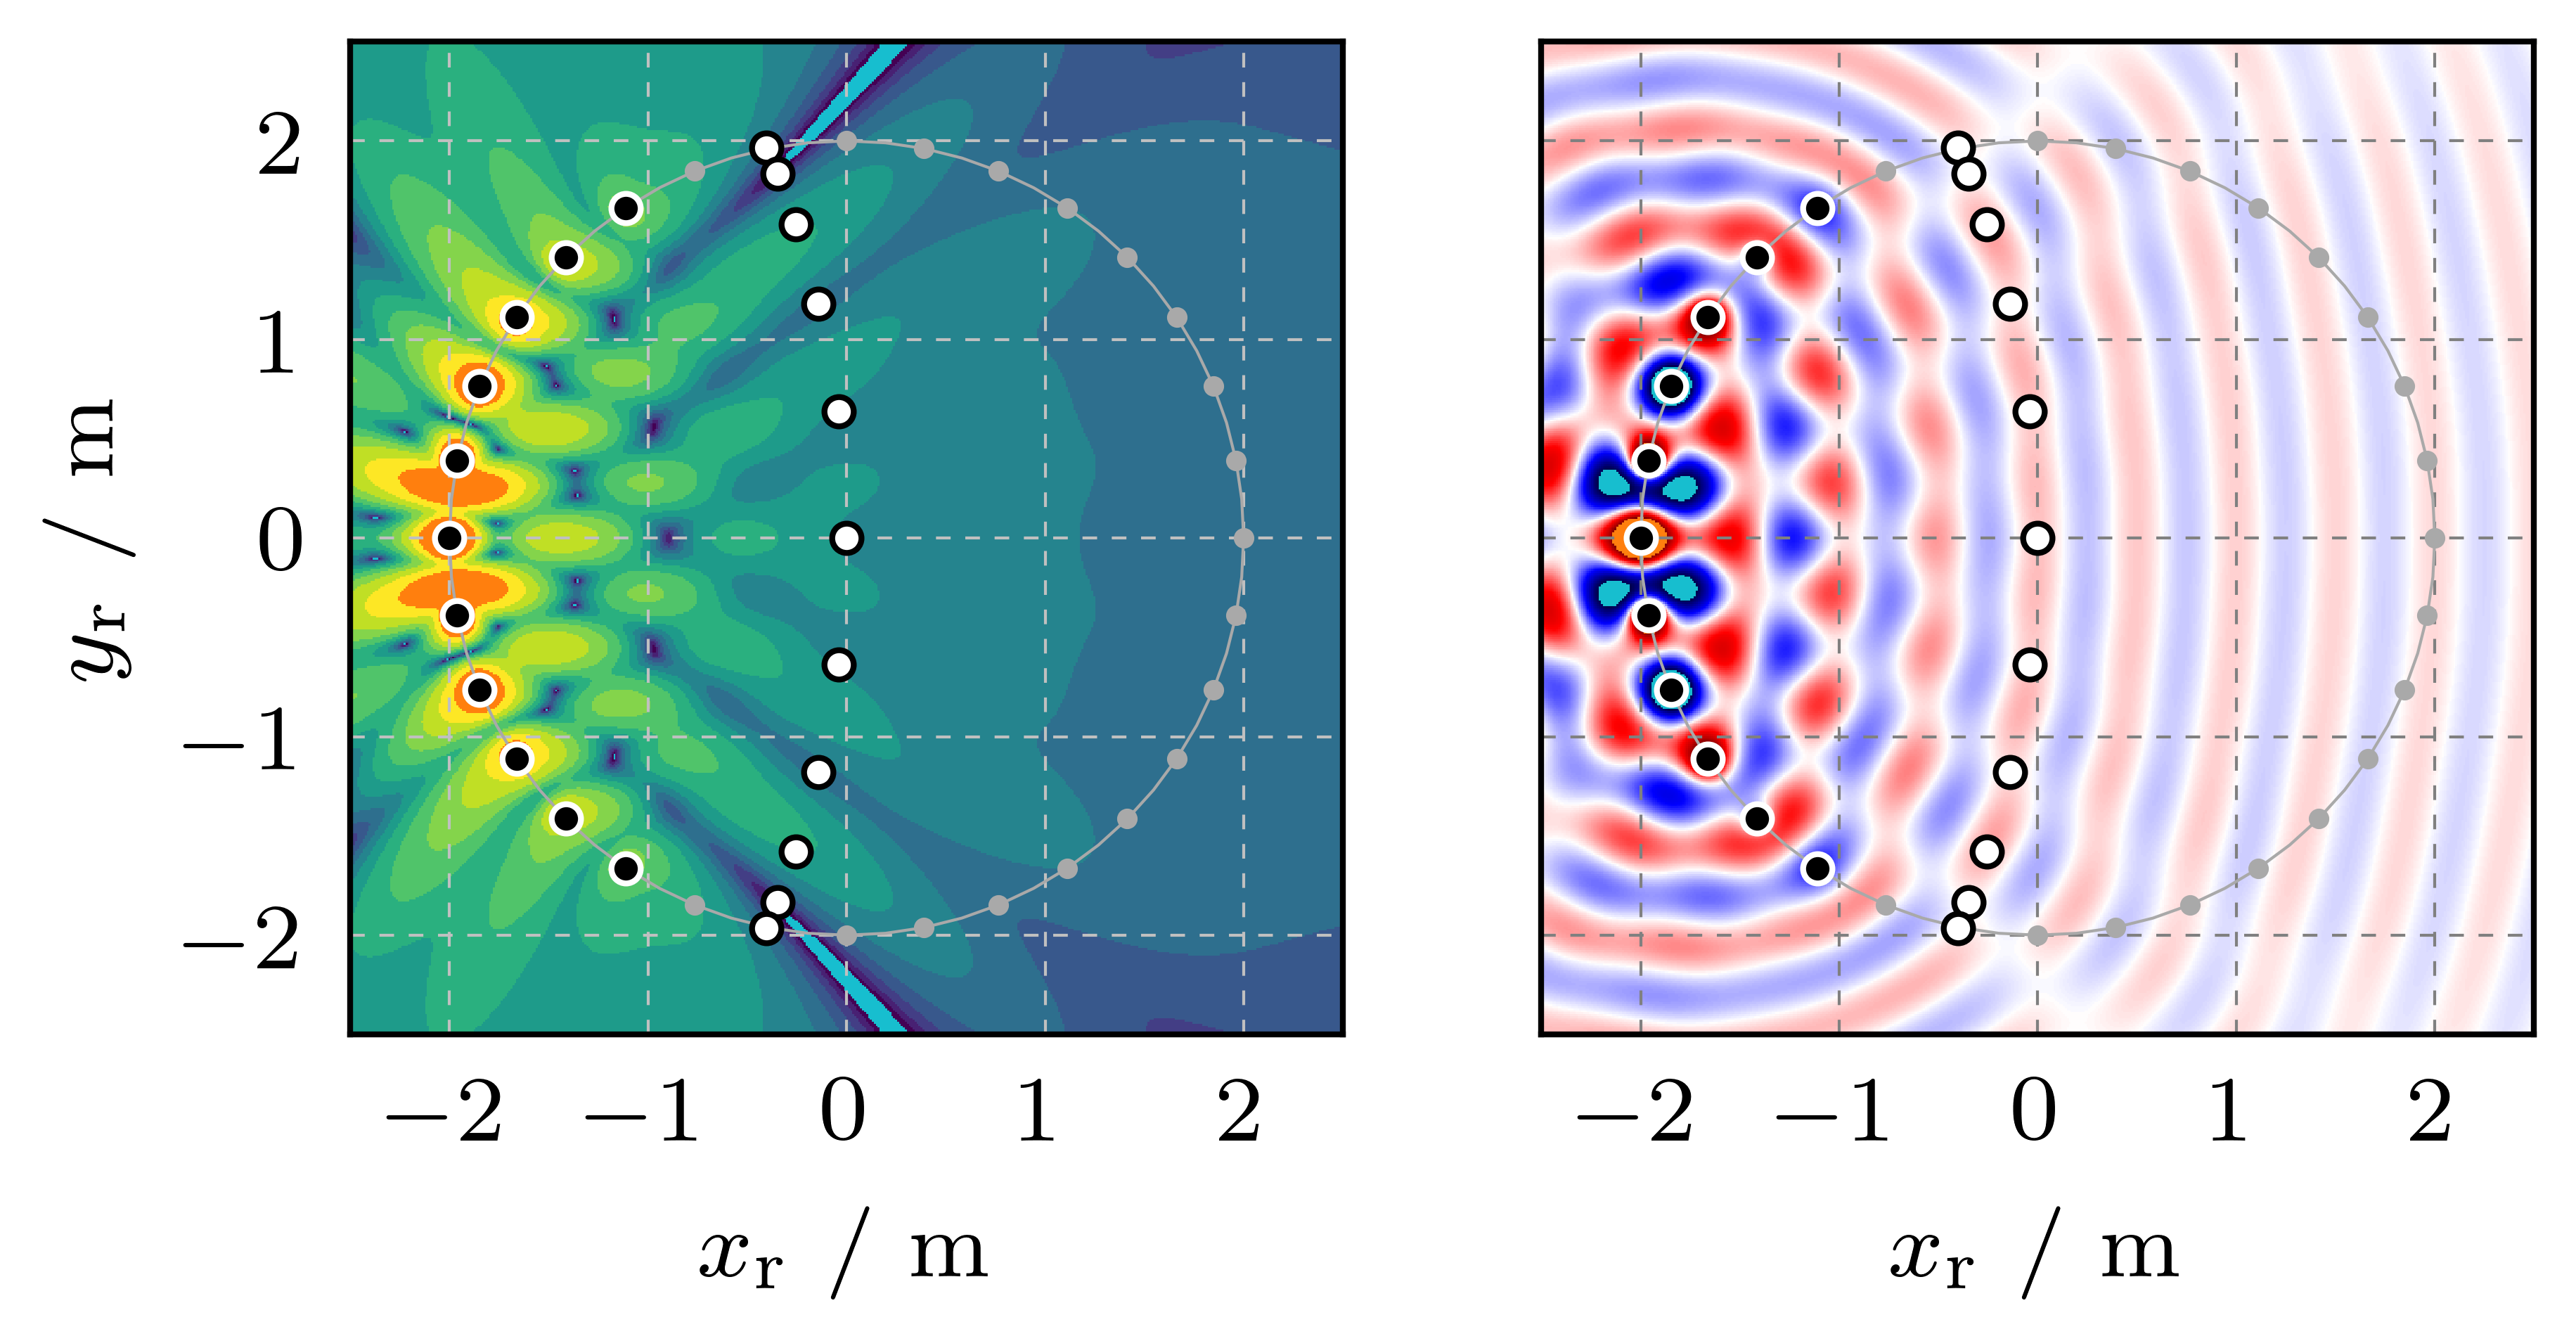
\includegraphics[width=85mm]{../python/wfs25d_circSSD_aliasing.png}
\end{plotfigures}
\caption{%2.5D-WFS einer virtuellen Punktquelle bei $\xp = (-5,0,0)^\mathrm{T}$\,m
%mit 32 äquiangular verteilten Monopolen auf einem 2\,m-Radius-Kreisarray
%für die Wellenlänge $\lambda=\frac{1}{2}$\,m.
2.5D WFS of a virtual point source at $\xp = (-5,0,0)^\mathrm{T}$\,m
with the wavelength $\lambda=\frac{1}{2}$\,m using a circular, discretised
monopole array (32 equiangularly spaced monopoles, radius 2 m).
%
%2.5D-WFS-Amplitudenkorrektur auf $0$\,dB-Pegel entlang des mittigen Kreisbogens.
Amplitude correction towards $0$\,dB level is applied for the arc shown in the
middle.
%
%Die 11 weißen Punkte auf diesem Kreisbogen bilden mit den 11 aktiven Monopolen
%(schwarze Punkte) jeweils ein Punktpaar mit stationärer Phasenbedingung.
There are eleven white dots along this arc-shaped reference curve,
each of which is related to one of the eleven active monopoles
(black dots).
These form eleven stationary phase point pairs.
%
%Bei der, zur sinnvollen Veranschaulichung, gewählten Frequenz gilt speziell, dass
%im linken bzw. rechten Teil der kreisförmigen Zuhörerfläche viel bzw. wenig
%Aliasingartefakte die gewünschte Wellenfront beeinträchtigen.
The frequency is chosen for illustrative purposes:
In the left/right part of the circular listener area,
many/few spatial aliasing artefacts, respectively,
interfere with the desired wavefront.
%
\cc
}
\label{fig:wfs25d_circSSD_aliasing}
\end{figure}



%In \myfig\ref{fig:wfs25d_circSSD_aliasing} ist ein weiteres aliasing-behaftetes
%Schallfeld dargestellt, bedingt durch ein räumlich diskretisiertes,
%kreisförmiges Array.
In \myfig\ref{fig:wfs25d_circSSD_aliasing}, another spatial-aliasing-affected
sound field is shown, caused by a spatially discretised circular array.
%
%Für den gewählten Radius ist die Verwendung von 32 bis 64 Lautsprechern
%praxisnah.
For the selected radius, using 32--64 loudspeakers is practical.
%
%Für die gewünschte gekrümmte Wellenfront einer virtuellen Punktquelle
%ist räumliches Aliasing rechts der gewählten Kreisbogen-Referenzkurve
%bei der gewählten Frequenz annähernd vernachlässigbar.
For the chosen frequency, the impact of spatial aliasing on the desired curved
wavefront of a virtual point source is only negligible in the right-hand part
of the plots.
%
%Für die betrachtete Frequenz enthält das Schallfeld links der Referenzkurve,
%also näher an den aktiven Monopolen, deutlich Aliasingartefakte.
For the frequency under consideration, the sound field in the left-hand
part of the plots, i.e. closer to the active monopoles, apparently
contains spatial aliasing artefacts.



%Während sich für planare, lineare, sphärische und zirkuläre Arrays
%die Entstehung räumlichen Aliasings mittels räumlicher Fourier-Transformation
%vergleichsweise bequem studieren lässt,
%vgl. \cite{Start1997_diss,Spors2008b,Ahrens2010_IEEE,Fazi2010,Schultz2016_diss},
%ist vor allem für kompliziertere Geometrien und damit einhergehend fehlender
%analytischer Lösungen ein akustisches Strahlenmodell\index{Schallstrahlenmodell}
%nützlich, vgl. \cite{Winter2019_diss}.
%
The formation of spatial aliasing can be conveniently and analytically
studied for planar, linear, spherical and circular arrays using their
spatial Fourier transforms, cf. \cite{Start1997_diss,Spors2008b,Ahrens2010_IEEE,
Fazi2010,Schultz2016_diss, Firtha2019_diss}.
However, analytical solutions are lacking for more complex geometries,
making a sound ray model\index{sound ray model} useful, cf. \cite{Winter2019_diss}.
%
%Dies kann vorteilhaft genutzt werden, um aliasing-freie Zonen über einen großen
%Frequenzbereich näherungsweise zu prädizieren ohne aufwändige Simulationen von
%Schallfeldern und Richtcharakteristiken durchführen zu müssen.
This can be used to predict spatial-aliasing-free zones over a wide
frequency range without having to perform complex simulations of
sound fields and far-field directivities.



%\subsection{Impulsartiges Schallfeld}
\subsection{Broadband Sound Fields}

%Die
%fig:td_0m_noaliasing %Abb.~\ref{fig:td_-1m},~\ref{fig:td_0m},~\ref{fig:td_1m}
%\myfig\ref{fig:td_0m_noaliasing} bis \ref{fig:td_1m}
%zeigen wie sich die 2.5D-WFS bei impulshafter Audiosignal-Anregung unter Benutzung
%des theoretischen WFS-Vorfilters in \myeq\eqref{eq:Prefilter25D} verhält.
The \myfigs\ref{fig:td_0m_noaliasing}--\ref{fig:td_1m}
show how a band-limited impulse as audio input is rendered by
the 2.5D WFS using the theoretical WFS prefilter
in \myeq\eqref{eq:Prefilter25D}.
%
%Die virtuelle Punktquelle wird zum Zeitpunkt
%$t=0$\,s mit einem auf $15$\,kHz tiefpassbegrenzten, zeitlichen Dirac-Impuls angeregt,
%welcher sich im Freifeld räumlich mit Schallgeschwindigkeit $c=343$\,m/s
%auf eine immer größer werdende Kugelfläche ausbreitet, also ein Monopol-Schallfeld mit
%$15$\,kHz-Bandbreite darstellt.
At time $t=0$\,s, the virtual point source is excited by a Dirac delta function
filtered with a $15$\,kHz low-pass filter.
In the free field, this impulse would be emitted omnidirectionally at the speed
of sound, thus representing the virtual sound field of a monopole with a flat
spectrum up to 15 kHz.



%Für die Synthese dieser 3D-Wellenfront mit einem räumlich diskretisierten 2D-Array
%und der 2.5D-Filter-Impulsantwort in \myeq\eqref{eq:h25d_time}
%sind ähnliche Artefakte wie bei monofrequenter Ansteuerung zu erwarten:
%a) 2.5D charakteristische Amplitudenabnahme
%über den Ausbreitungsweg,
%b) frequenzabhängiger Nah-/Fernfeldübergang und
%c) frequenzabhängiges räumliches Aliasing.
Similar artefacts to those seen at single frequencies are to be expected
when synthesising this 3D wavefront with the 2.5D driving signals
\eqref{eq:h25d_time} using a spatially discretised 2D array:
a) 2.5D characteristic amplitude decay along the propagation path,
b) a frequency-dependent near-field/far-field transition and
c) frequency-dependent spatial aliasing.



%\myfig\ref{fig:td_0m_noaliasing} bis \ref{fig:td_1m} zeigen
%jeweils rechts die impulshafte Wellenfront in der $xy$-Ebene zu einem
%bestimmten Ausbreitungszeitpunkt,
%jeweils links/oben die Antwort des akustischen Systems auf den tiefpassbegrenzten,
%zeitlichen Eingangsimpuls, die mit einem Messmikrofon am Aufpunkt $\times$ gemessen
%würde und
%jeweils links/unten den zugehörigen Frequenzgang.
The \myfigs\ref{fig:td_0m_noaliasing}--\ref{fig:td_1m} depict,
on the right plot,
the impulsive wavefront in the $xy$-plane at a specific propagation time,
on the left/top plot,
the acoustic system's response to the input impulse, which would be measured
with a microphone at the probe point $\times$,
and on the left/bottom plot,
its corresponding spectrum.
For convenience, it is referred to as the acoustic system's impulse response and
frequency response in the following, even though the excitation is
performed with a low-pass filtered impulse.
%
%Die Simulationen erfolgten mit Abtastfrequenz $f_s = 192$\,kHz.  % not included in GER and ENG version



% please DO NOT rescale the figure and keep it double column
\begin{figure*}
\centering
\begin{plotfigures}
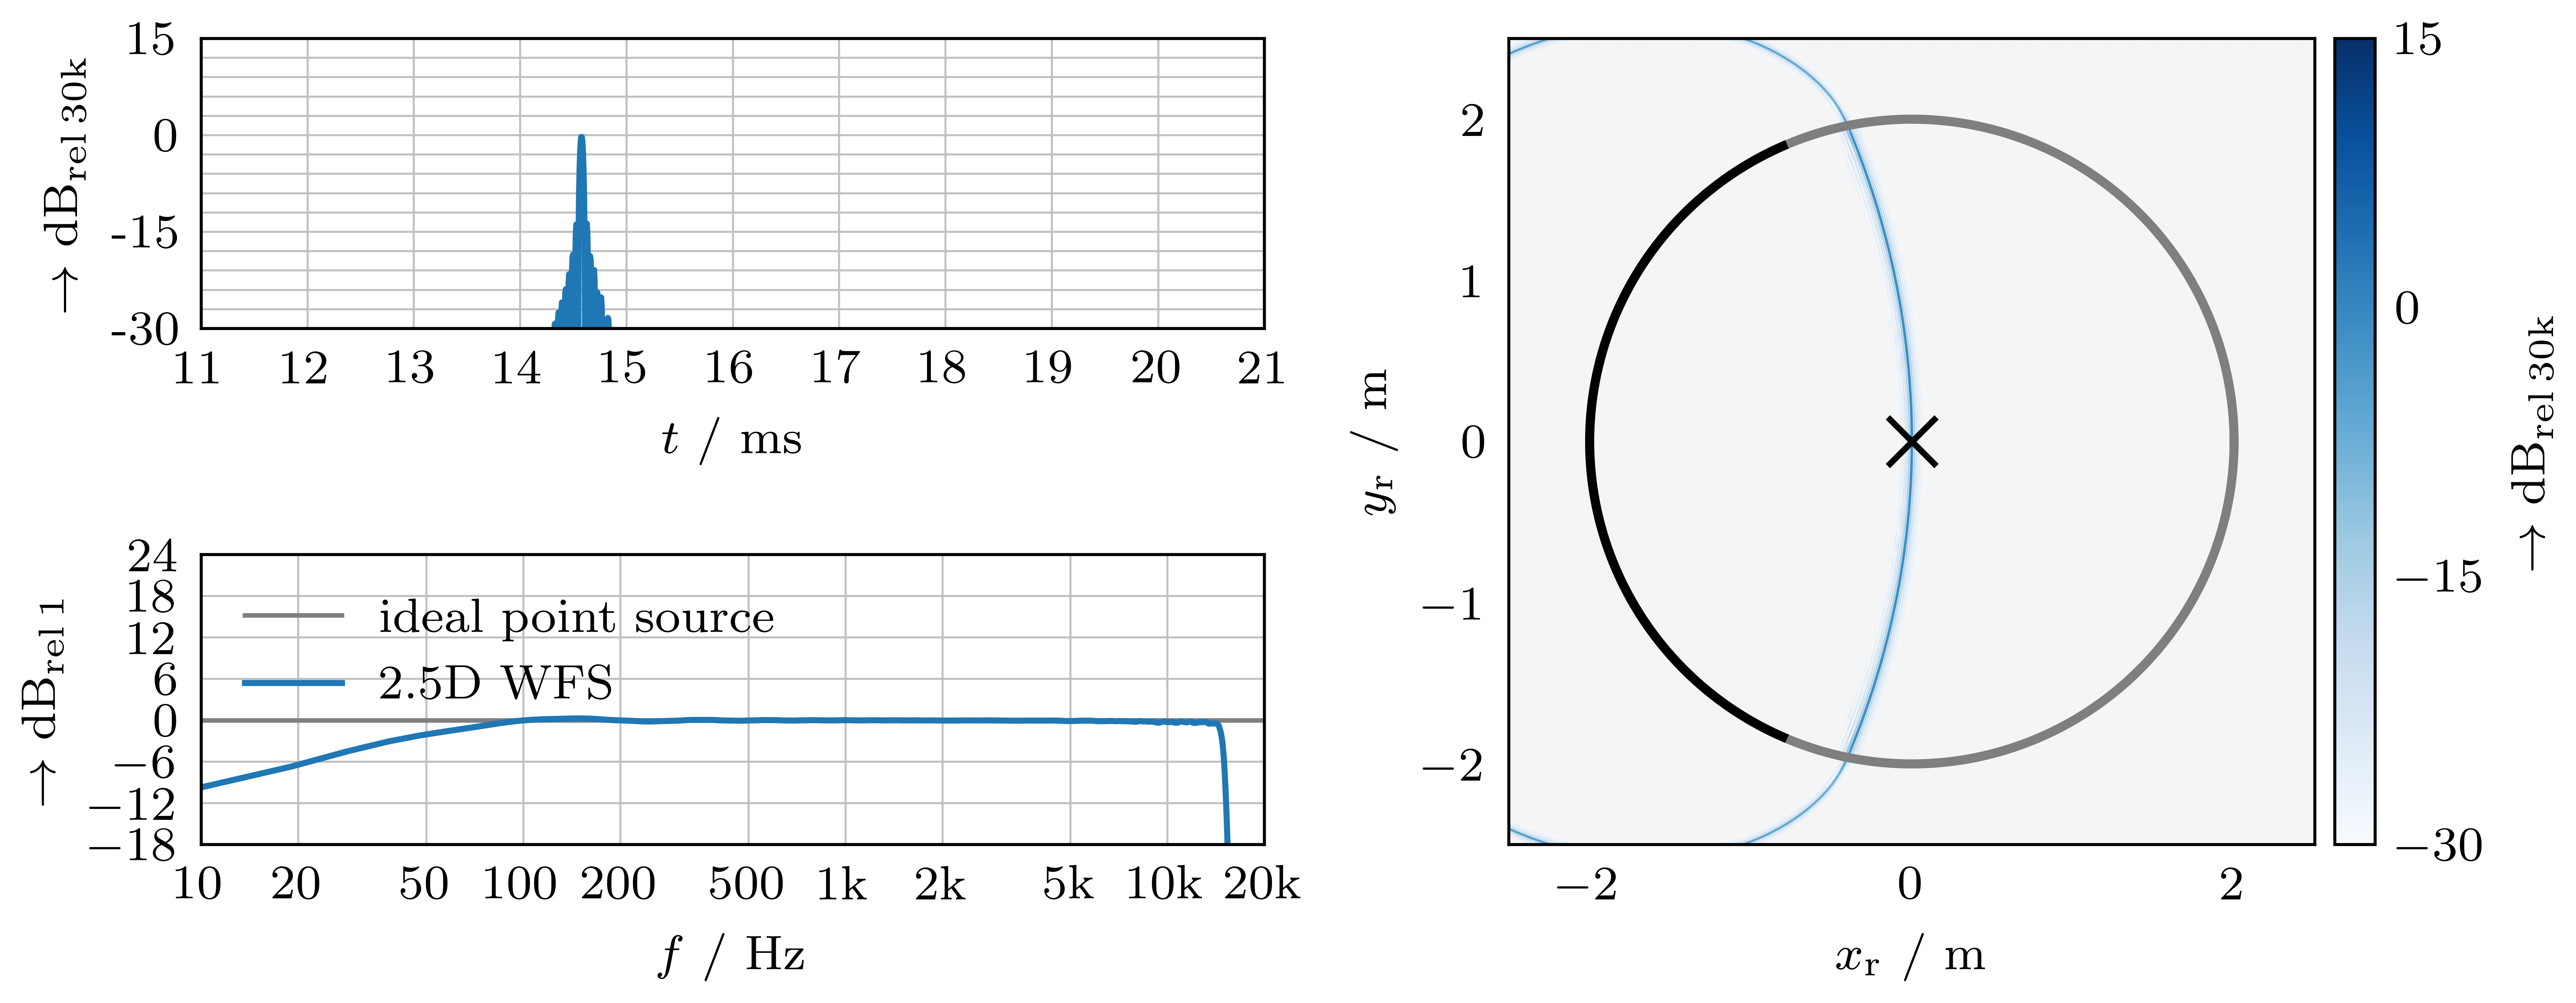
\includegraphics[width=145mm]{../python/wfs25d_circSSD_noaliasing_time_domain_x0.00_m_py_ENG.png}
\end{plotfigures}
\caption{%2.5D-WFS-Schallfeld bei impulshafter Anregung zum Zeitpunkt $t=0$\,s
%(rechts) für das Szenario aus \myfig\ref{fig:wfs25d_circSSD_aliasing}, allerdings
%hier mit kontinuierlichem Kreisarray, aktiver Teil des Arrays in schwarz,
%inaktiver Teil in grau.
2.5D WFS sound field (right) due to impulsive excitation at time $t=0$\,s
for the setup shown in \myfig\ref{fig:wfs25d_circSSD_aliasing},
but with a continuous array.
The active part of the array is shown in black, while the
inactive part is shown in dark grey.
%
%Hier und in \myfig\ref{fig:td_-1m} bis \ref{fig:td_1m} gilt für die
%rechte Grafik des impulshaften Schallfelds:
Here and in \myfigs\ref{fig:td_-1m}--\ref{fig:td_1m},
the following applies to the right-hand graph of the impulsive sound field:
%
%Pegel $>+15\,\text{dB}$ erfahren eine Farbsättigung mit schwarz,
%Pegel $<-30\,\text{dB}$ hingegen mit grau.
Level $>+15$\,dB is saturated to black,
level $<-30$\,dB is saturated to grey.
%
%Der dargestellte Zeitpunkt $t \approx 14{,}578$\,ms entspricht der
%Schallausbreitungszeit der virtuellen Punktquelle zum Messpunkt $\times$ bei
%$\xr=(0,0,0)^\mathrm{T}$\,m für die Schallgeschwindigkeit $c=343$\,m/s.
The snapshot shown corresponds to the time $t \approx 14{.}578$\,ms
during which the sound propagated from the virtual point
source to the measurement point at $\xr=(0,0,0)^\mathrm{T}$\,m,
assuming a speed of sound of $c=343$\,m/s.
%
%Akustische Impulsantwort (links, oben) und Frequenzgang (links, unten)
%am Messpunkt $\times$.
For the measurement point marked with $\times$,
the acoustic impulse response is shown in the upper-left diagram
and the frequency response in the lower-left diagram.
%
%Die perfekt synthetisierte Wellenfront ist koinzident mit der Referenzkurve,
%daher im Frequenzgang gewünschter $0$\,dB-Referenzpegel
%zwischen ca. $100$\,Hz und $15$\,kHz.
The perfectly synthesised wavefront coincides with the reference curve,
resulting in a frequency response of $0$\,dB between approximately
$100$\,Hz and $15$\,kHz.
%
%Impulsspezifischer Pegel in $\text{dB}_{\text{rel }30\text{k}}$ relativ zum
%endlichen Amplitudenwert $30{.}000$ des zeitkontinuierlichen, $15$\,kHz-tiefpassbegrenzten Anregeimpulses.
The dB scale used to depict the acoustic impulse responses originates from the
continuous-time low-pass filter with a cut-off frequency of $15$\,kHz,
meaning the band-limited sinc-shaped excitation impulse exhibits
a maximum peak of 30,000; hence the notation $\text{dB}_{\text{rel\,}30\text{k}}$.
%
\cc
}
\label{fig:td_0m_noaliasing}
\end{figure*}



%\myfig\ref{fig:td_0m_noaliasing} zeigt das Ergebnis einer Simulation mit einem
%kontinuierlichen Kreisarray.
\myfig\ref{fig:td_0m_noaliasing} shows the result of a simulation using a
continuous circular array.
%
%Es treten daher nur die Artefakte der Punkte a) und b) auf.
Therefore, only the artefacts related to items a) and b) can occur,
but no spatial aliasing.
%
At the selected time, the wavefront matches the chosen
reference curve for amplitude-corrected synthesis.
%
%Für den Frequenzbereich $100\,\text{Hz} < f < 15\,\text{kHz}$
%wird eine nahezu perfekte Wellenfront synthetisiert.
A nearly perfect wavefront is synthesised for the frequency
range $100\,\text{Hz} < f < 15\,\text{kHz}$.
%
%Zum dargestellten Zeitpunkt ist die Wellenfront koinzident mit der gewählten
%Referenzkurve.
%At the selected time, the wavefront matches the chosen
%reference curve for amplitude-corrected synthesis. -> kommt sinnvollerweise ein Satz früher
% phrase moved up for more streamlined story
%
%Der Frequenzgang entspricht daher dem gewünschten $0$\,dB-Referenzpegel in diesem
%Frequenzbereich.
The frequency response corresponds to the desired reference level of $0$\,dB
within this frequency range.
%
%Unterhalb $100$\,Hz tritt Hochpassverhalten auf.
Below 100 Hz, a low-frequency roll-off is observed.
%
%In diesem Beispiel sind dafür zwei Aspekte konfundiert verantwortlich.
In this example, this is due to two interrelated aspects.
%
%Zum einen sind für kleiner werdende Frequenzen
%die zugehörigen Wellenlängen zunehmend größer als die Apertur\index{Apertur}.
As the frequencies decrease, the corresponding wavelengths become considerably
larger than the aperture\index{aperture}.
%
%Das Array bietet für diese Wellenlängen keine Kontrolle von Interferenz
%in einem ausgedehnten Nahfeld, es strahlt in vergleichsweise naher Entfernung
%schon ins Fernfeld ab.
For these wavelengths, the array offers no control of interference
for the near field.
The array already radiates into the far field at comparatively close distances.
%
%Zum anderen gilt die Fernfeld-/Hochfrequenznäherung $\wc r_{\xs\text{-}\xr} \gg 1$
%für die tiefen Frequenzen und den gewählten Aufpunkt nicht.
On the other hand, the far-field/high-frequency approximation
$\wc r_{\xs\text{-}\xr} \gg 1$ does not apply to the low frequencies
and the selected probe point.
%
%Es ist also zu erwarten, dass die tatsächliche physikalische Synthese von der
%gewünschten WFS-Lösung abweicht.
Therefore, it is to be expected that the actual physical synthesis will
deviate from the desired synthesis solution.



% please DO NOT rescale the figure and keep it double column
\begin{figure*}
\centering
\begin{plotfigures}
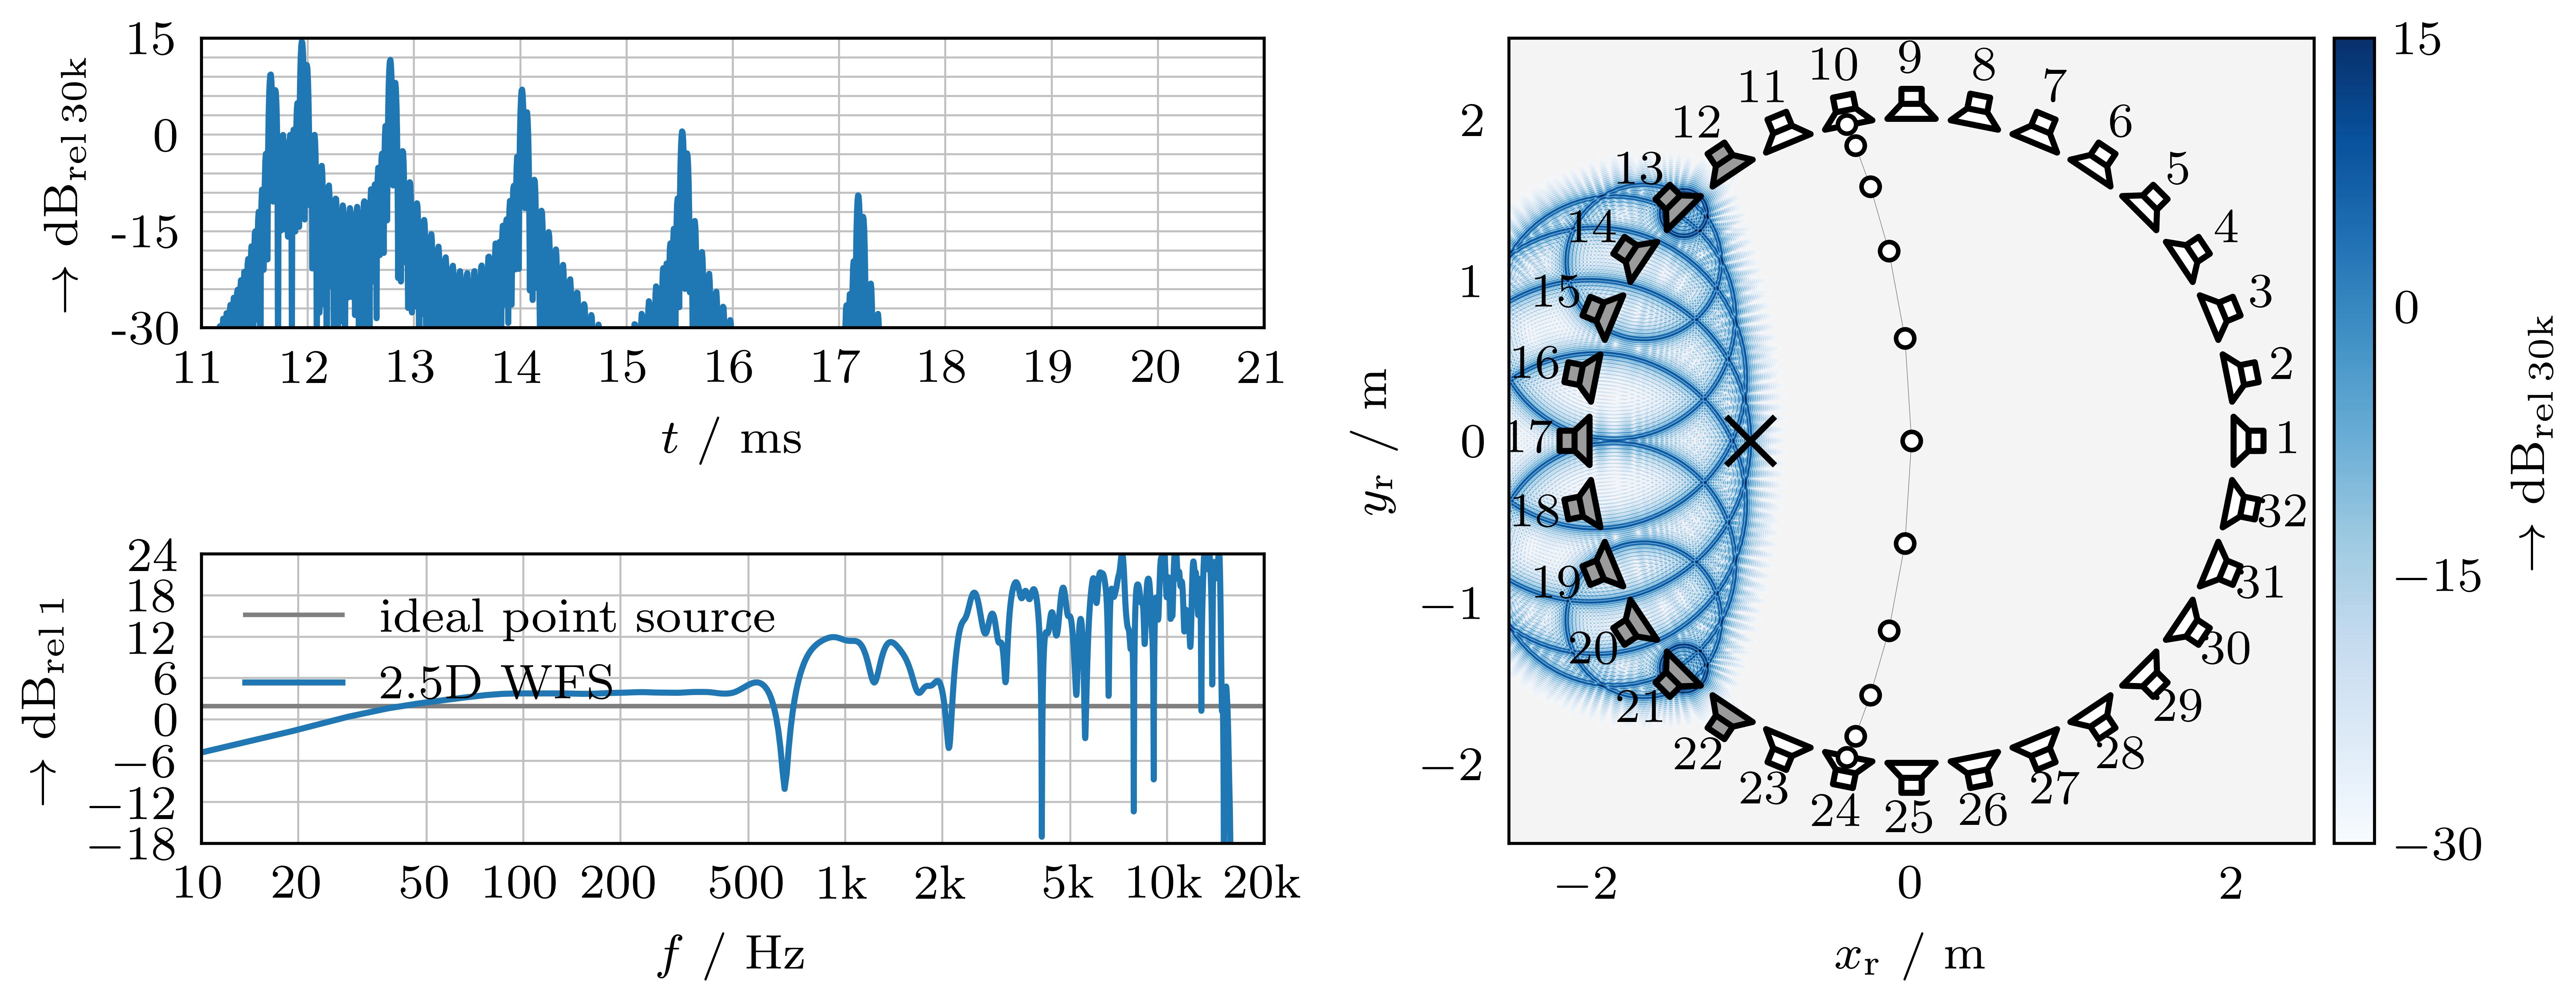
\includegraphics[width=145mm]{../python/wfs25d_circSSD_aliasing_time_domain_x-1.00_m_py_ENG.png}
\end{plotfigures}
\caption{%2.5D-WFS-Schallfeld (rechts) bei impulshafter Anregung zu $t=0$\,s für das
%Szenario aus \myfig\ref{fig:wfs25d_circSSD_aliasing}.
2.5D WFS sound field (right) due to impulsive excitation at time $t=0$\,s
for the setup shown in \myfig\ref{fig:wfs25d_circSSD_aliasing}.
%
%Pegelreferenzkurve als Kreisbogen durch $\xr=(0,0,0)^\mathrm{T}$\,m (rechts).
Amplitude-corrected synthesis occurs at the arc-shaped reference curve passing
through $\xr=(0,0,0)^\mathrm{T}$\,m.
%
%Dargestellter Zeitpunkt $t\approx 11{,}662$\,ms bei Schallgeschwindigkeit
%$c=343$\,m/s entspricht der Wellenlaufzeit der virtuellen Punktquelle zum
%Messpunkt $\times$ bei $\xr=(-1,0,0)^\mathrm{T}$\,m.
The specified time $t\approx 11{.}662$\,ms corresponds to the sound
propagation from the virtual point source to the measurement point $\times$ at
$\xr=(-1,0,0)^\mathrm{T}$\,m, for which
%
%Akustische Impulsantwort (links, oben) und Frequenzgang (links, unten) vom Messpunkt $\times$.
the acoustic impulse response is shown in the upper-left plot
and the frequency response in the lower-left plot.
%
\cc
}
\label{fig:td_-1m}
\end{figure*}



%\myfig\ref{fig:td_-1m} bis \ref{fig:td_1m} entsprechen dem Szenario aus
%\myfig\ref{fig:wfs25d_circSSD_aliasing}, d.h. einem räumlich diskretisierten
%Kreisarray mit 32 Monopolen.
The \myfigs\ref{fig:td_-1m}--\ref{fig:td_1m} correspond to the setup
shown in \myfig\ref{fig:wfs25d_circSSD_aliasing}, i.e. a spatially
discretised circular array with 32 monopoles.
%
%Durch die räumliche Diskretisierung des Arrays entstehen für $f>f_\text{max}$
%räumliche Aliasingartefakte, die in den drei Darstellungen unterschiedlich
%repräsentiert werden: entweder als nicht geschlossene Wellenfront bzw.
%als eine Wellenfronteinhüllende (rechts),
%als zeitliche Folge von Impulsen (links/oben, im Folgenden wegen der
%Tiefpassbegrenzung technisch zwar ungenau aber wesentlich korrekt als
%Impulsantwort bezeichnet) oder als hochfrequente Frequenzgangsverzerrungen
%(links/unten).
The spatial discretisation of the array causes
spatial aliasing\index{spatial aliasing} artefacts for $f>f_\text{max}$.
These are illustrated differently in the three subplots of each figure:
The plot on the right shows a wavefront envelope instead of a closed wavefront.
The upper-left diagram shows that the impulse response consists of a sequence
of impulses.
The frequency response in the lower-left plot reveals deviations from a flat
spectrum, particularly at higher frequencies.

%Insgesamt sind wie auch in \myfig\ref{fig:wfs25d_circSSD_aliasing} elf Monopole, die
%Lautsprecher (LS) 12--22, gemäß des \textit{secondary source selection criterion}
%nach \myeq\eqref{eq:SecSrcSel} an der Synthese beteiligt und definieren die Apertur.
As in \myfig\ref{fig:wfs25d_circSSD_aliasing}, a total of eleven monopoles,
i.e. the loudspeakers (LS) 12--22, are involved in the synthesis.
These define the aperture due to the secondary source selection
\myeq\eqref{eq:SecSrcSel}.
%
%Die anderen Lautsprecher werden für die gewählte Parametrik der virtuellen Quelle
%nicht benötigt und daher nicht angesteuert.
The other loudspeakers are not required for the chosen virtual source parameters
and are therefore not activated.
%
% sentence moved to here from the bottom of this paragraph:
The resulting impulse responses of this 2.5D WFS scenario are not compact in
time and represent spatial aliasing in the time domain.
%
%In den Impulsantworten dieses 2.5D-WFS-Szenarios lässt sich immer eine Abfolge von
%sechs Impulsen in der Impulsantwort erkennen.
The impulse responses of the three examples always contain a sequence of six
impulses.
%
%Der erste stammt von LS 17.
The first impulse is assigned to LS 17.
%
%Dieser befindet sich auf der $x$-Achse in Linie mit der
%Primärquellenposition und allen drei gezeigten Messpunkten, ist für diese also
%genau der Monopol mit stationärer Phasenbedingung und weist die kürzeste
%Distanz zur virtuellen Quelle auf.
This loudspeaker is located on the $x$-axis, in line with the
position of the virtual source and the three probe points $\times$.
Therefore, it is the loudspeaker that is closest to the virtual source.
It is also the one that fulfils the stationary phase condition with the
three measurement points.
%
%Es folgen zeitlich fünf Impulse nach, die den, wegen des Delays in der
%Treiberfunktion, verzögert spielenden Monopolen zuordenbar sind.
The following five impulses are attributed to the delays in the
corresponding loudspeakers' driving function.
%
%Der zweite Impuls wird demzufolge von den LS 16 und 18 zu exakt gleichen
%Anteilen erzeugt und hat höhere Amplitude als der Erstimpuls.
LS 16 and 18, therefore, generate the second impulse in equal proportions,
yielding a higher amplitude than that of the first impulse.
%
%Der letzte Impuls stammt entsprechend von LS 12 und 22.
The last impulse comes from LS 12 and 22, respectively.
%
%Diese paarweise Koinzidenz entsteht durch die gewählte Geometrie:
This coincidental loudspeaker pairing is the result of the chosen
geometry and setup:
%
%das Array ist symmetrisch zur $x_\mathrm{r}$-Achse, auf der wie
%erwähnt auch die Primärquelle und die Messpunkte positioniert sind.
The array is symmetrical to the $x$-axis,
and, as already mentioned, the virtual source and the probe
points are also located on this axis.
%
%Das sechsfach Impulsmuster ist also für alle Messpunkte auf der
%horizontalen Symmetrieachse gleich, allerdings ändern sich über die
%Entfernung vom aktiven Array die relativen Zeitbezüge der Impulse.
The observed sixfold impulse pattern is therefore the same for all
probe points on the horizontal axis of symmetry.
However, the relative timing of the impulses changes
with increasing distance from the active array.
%
%Der Erstimpuls hingegen lässt sich zeitlich immer exakt bezüglich der
%Schallgeschwindigkeit $c$ und Position der virtuellen Punktquelle
%verorten.
On the other hand, the absolute timing of the first impulse can
always be precisely determined in terms of the speed of sound $c$
and the position of the virtual point source $\xp$.
%
%Die resultierenden, zeitlich nichtkompakten Impulsantworten repräsentieren
%räumliches Aliasing im Zeitbereich.
%The resulting impulse responses are not compact in time and represent
%spatial aliasing in the time domain. -> Satz nach oben, phrase moved up



% please DO NOT rescale the figure and keep it double column
\begin{figure*}
\centering
\begin{plotfigures}
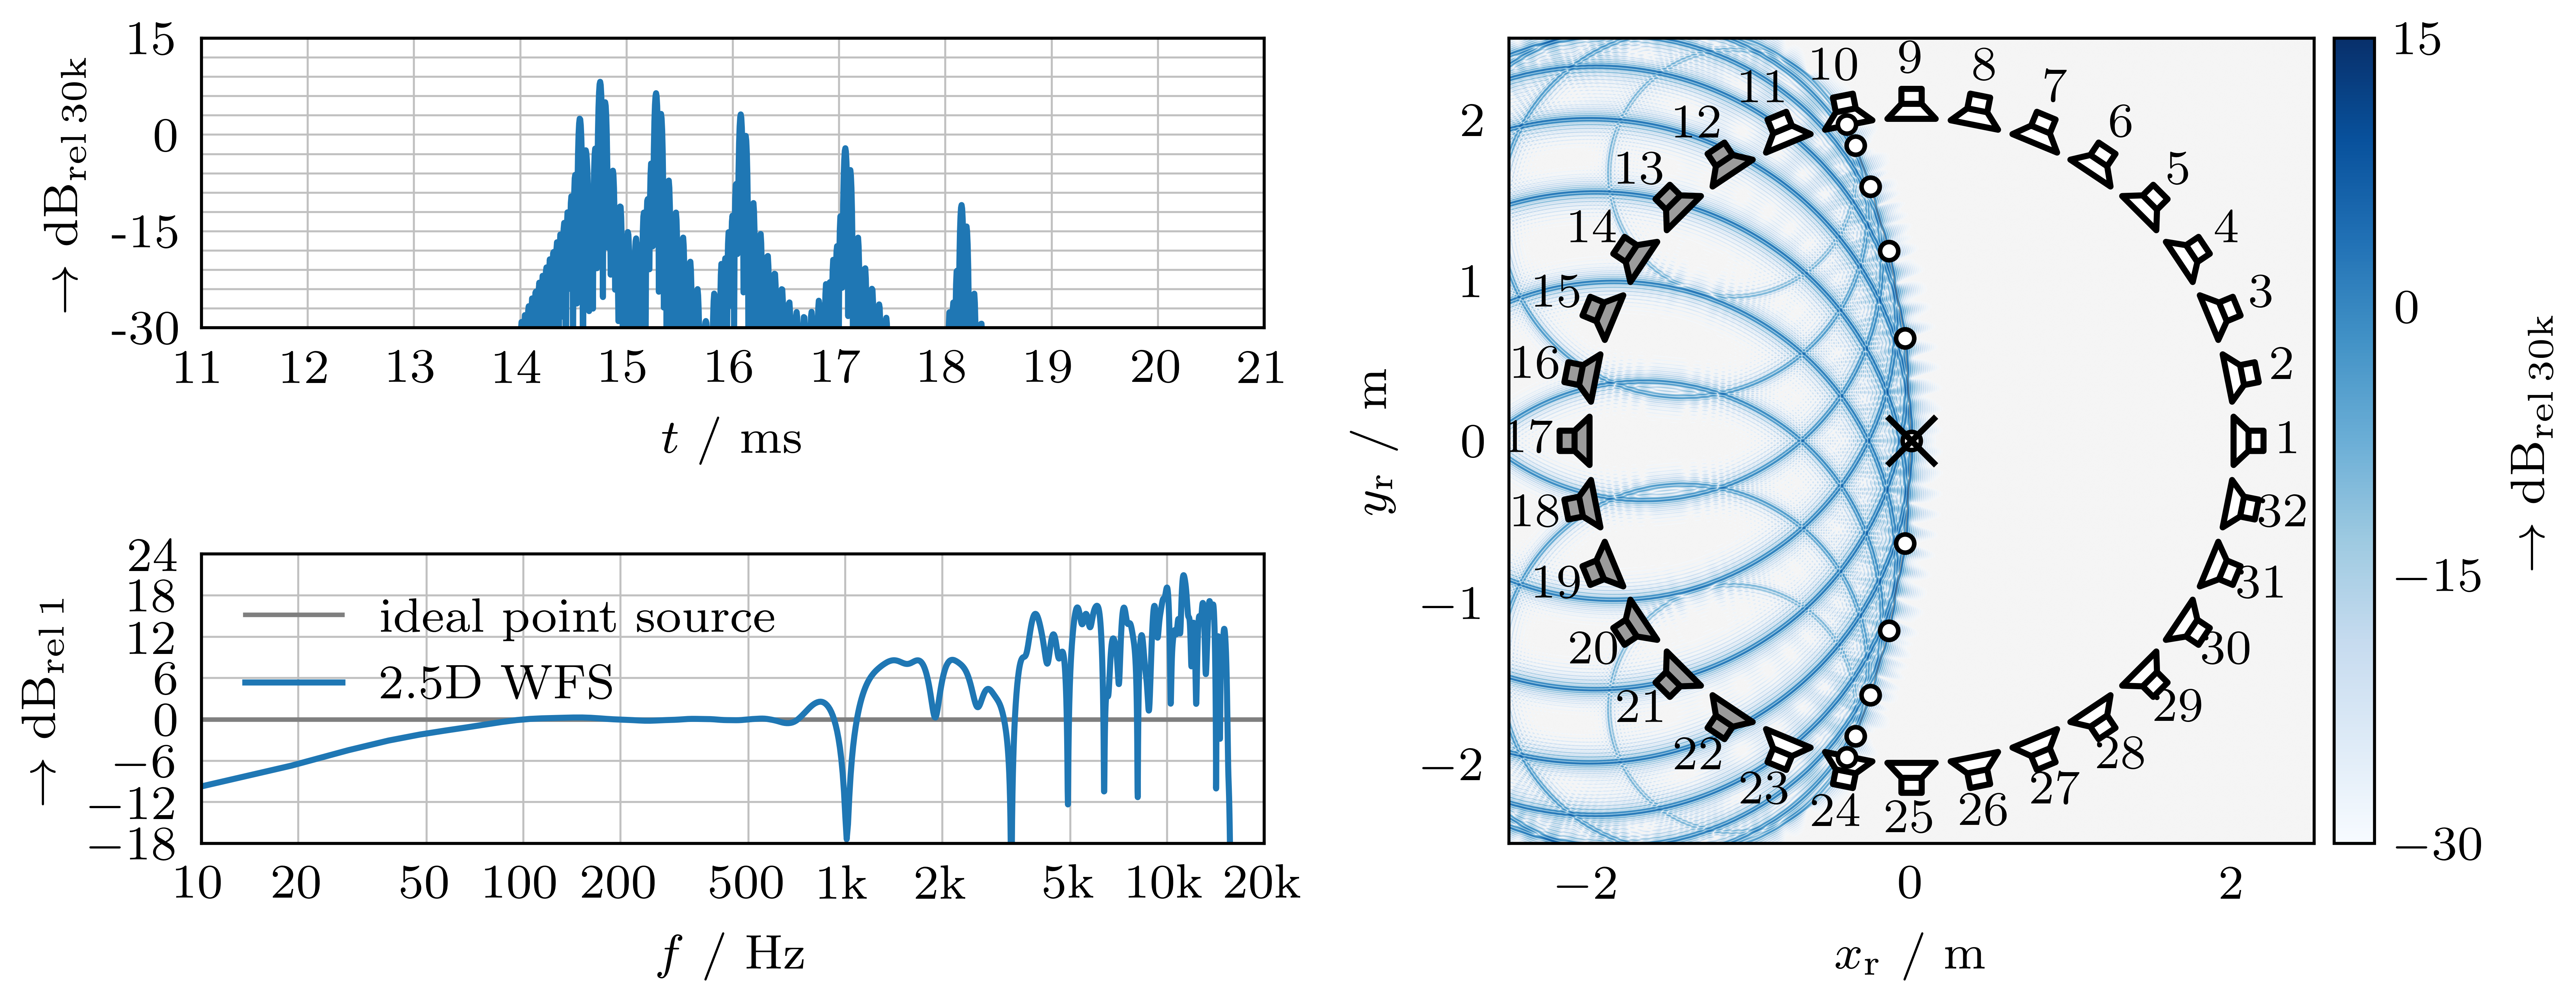
\includegraphics[width=145mm]{../python/wfs25d_circSSD_aliasing_time_domain_x0.00_m_py_ENG.png}
\end{plotfigures}
\caption{%2.5D-WFS-Schallfeld
%ähnlich \myfig\ref{fig:td_-1m} für Zeitpunkt $t \approx 14{,}578$\,ms,
%Messpunkt $\times$ bei $\xr=(0,0,0)^\mathrm{T}$\,m.
2.5D WFS sound field similar to \myfig\ref{fig:td_-1m} for specified time
$t \approx 14{.}578$\,ms and measurement point $\times$ at
$\xr=(0,0,0)^\mathrm{T}$\,m.
%
%Wellenfront ist koinzident mit der Pegelreferenzkurve, daher
%
%im Frequenzgang gewünschter (aliasing-freier) $0$\,dB-Referenzpegel zwischen ca. $100$ und $600$\,Hz.
%
The wavefront is coincident with the arc-shaped reference curve,
thus yielding flat $0$\,dB frequency response between
approximately $100$ and $600$\,Hz.
%
\cc
}
\label{fig:td_0m}
\end{figure*}



% please DO NOT rescale the figure and keep it double column
\begin{figure*}
\centering
\begin{plotfigures}
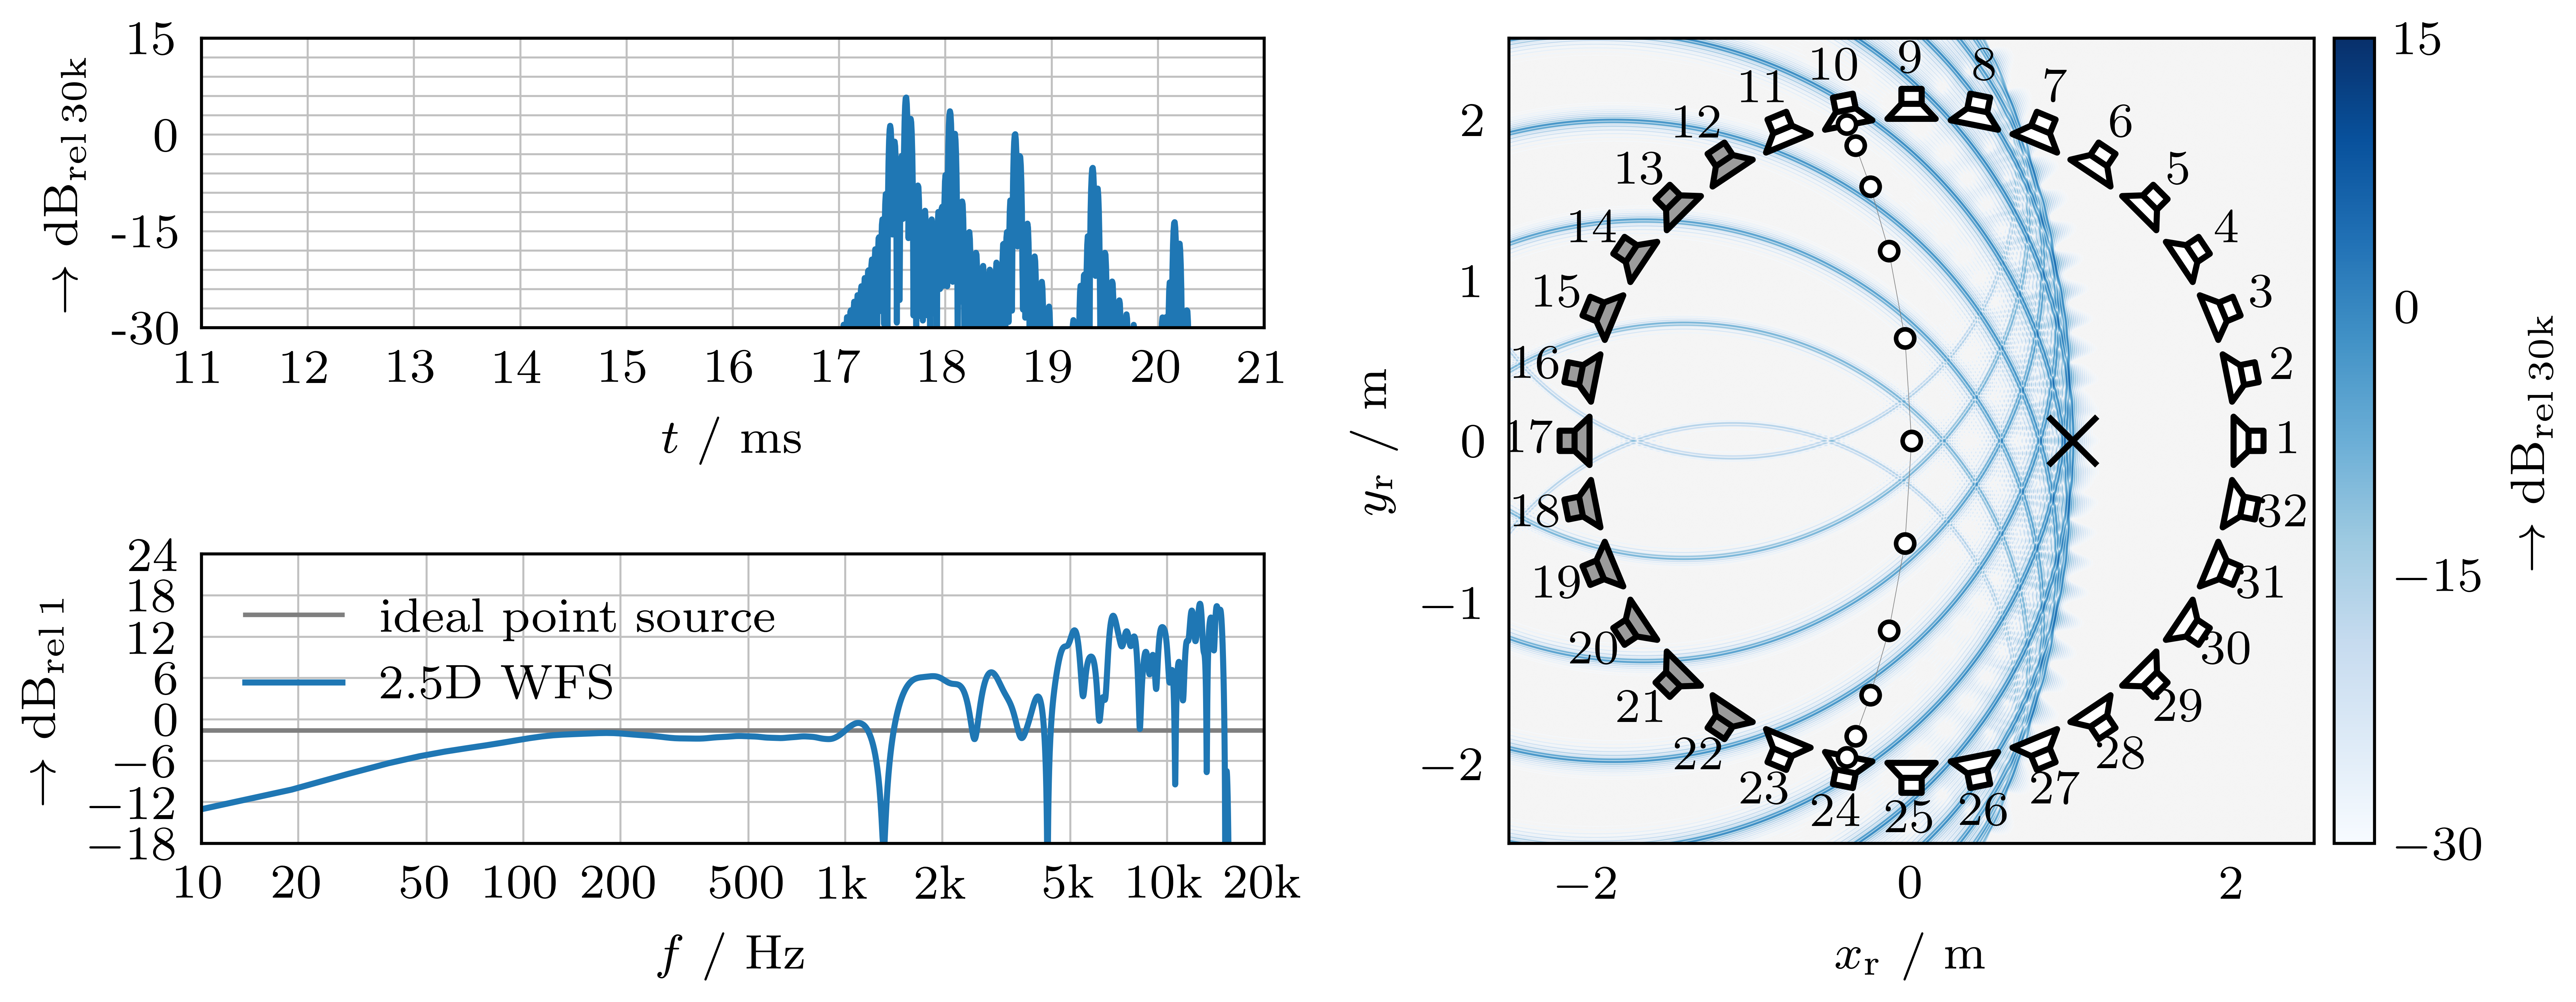
\includegraphics[width=145mm]{../python/wfs25d_circSSD_aliasing_time_domain_x1.00_m_py_ENG.png}
\end{plotfigures}
\caption{%2.5D-WFS-Schallfeld
%ähnlich \myfig\ref{fig:td_-1m} für Zeitpunkt $t \approx 17{,}493$\,ms,
%Messpunkt $\times$ bei $\xr=(1,0,0)^\mathrm{T}$\,m.
2.5D WFS sound field similar to \myfig\ref{fig:td_-1m} for specified time
$t \approx 17{.}493$\,ms and measurement point $\times$ at
$\xr=(1,0,0)^\mathrm{T}$\,m.
%
\cc
}
\label{fig:td_1m}
\end{figure*}



%Räumliches Aliasing aus Sicht der zugehörigen Spektren offenbart
%hochfrequent stark positionsabhängige Abweichungen vom gewünschten linearen
%Frequenzgang.
From the perspective of the associated frequency responses,
spatial aliasing reveals high-frequency deviations from the desired flat spectrum.
The deviations depend heavily on the listening position.
%
%Das für ein Kreisarray näherungsweise geltende Kriterium nach \myeq\eqref{eq:SamplingCriterion}
%zur vollständigen
%Vermeidung von Aliasing
%führt mit der Kreisbogenlänge
%$\Delta_{\xs}=0{,}3927$\,m zur Grenzfrequenz
%$f_\text{max} = \frac{c}{2 \Delta_{\xs}}\approx 437$\,Hz,
% 343 / (2 * (2 * pi * 360/2^5 / 180))
%oberhalb derer Aliasingartefakte im Frequenzgang zu erwarten sind.
The condition \myeq\eqref{eq:SamplingCriterion} holds approximately for a
circular array when the arc length $\Delta_{\xs}$ is used.
The arc length $\Delta_{\xs}=0{.}3927$\,m determines the cut-off frequency
$f_\text{max} = \frac{c}{2 \Delta_{\xs}}\approx 437$\,Hz, above which spatial
aliasing artefacts occur.
%
%Tatsächlich ist die Frequenz $f_\text{al}$ ab der Aliasing auftritt,
%vom Messpunkt und der Array-Geometrie abhängig, und
%kann $f_\text{al}>f_\text{max}$, aber niemals $f_\text{al}<f_\text{max}$ sein.
In fact, the actual cut-off frequency depends on the measurement point
and the finite-length array geometry.
It can be $f_\text{al}>f_\text{max}$, but never will
be $f_\text{al}<f_\text{max}$.
%
%Dies lässt sich verknüpfen mit der obigen Beobachtung: das Schallfeld
%weist für mittig vom Array entferntere Messpunkte (höhere $f_\text{al}$) geringere
%Aliasingartefakte auf, als nähere Messpunkte (niedrigere $f_\text{al}$).
This can be linked to the above observation that the sound field exhibits fewer
aliasing artefacts for measurement points further away from the centre of
the array (i.e. a higher $f_\text{al}$) than for measurement points closer to
the array (i.e. a lower $f_\text{al}$).



%Charakteristisch für Aliasingartefakte
%im Frequenzgang sind a) zahlreiche Anti-Resonanzen (Notches) und Resonanzen,
%deren spektrale Lage von der Messposition abhängt und
%b) eine steigende Flanke mit $+3$\,dB/Oktave,
%vgl. \cite{Spors2010a}.
In the frequency response, the spatial-aliasing artefacts are characterised
by a) numerous anti-resonances (notches) and resonances whose spectral positions
depend on the measurement position,
and by b) a rising slope with $+3$\,dB/octave and cut-off frequency $f_\text{al}$,
cf. \cite{Spors2010a}.
%
%Dies wird typisch als Klangverfärbung (\textit{colouration})
%wahrgenommen, vgl. \cite{Start1997_diss, Wittek2007_JAES, Wierstorf2014_diss,
%Winter2019_diss, Erbes2020_diss}.
This is typically perceived as sound colouration, cf. \cite{Start1997_diss,
Wittek2007_JAES, Wierstorf2014_diss, Winter2019_diss, Erbes2020_diss}.
%
%Es wird speziell dann sehr deutlich als sogenanntes Phasing wahrgenommen,
%wenn sich der Frequenzgang über die Zeit sehr stark ändert, etwa weil sich
%virtuelle Quelle und/oder Zuhörende (schnell) bewegen.
It is particularly noticeable in a phenomenon known as `phasing', which
occurs when the frequency response changes significantly and rapidly over
time.
This can be caused by quick movements of either the virtual source or the
listener.



%Der Frequenzgang der drei Beispiele ist zwischen ca. $100$ und $600$\,Hz
%annähernd linear und variiert über die Messpunkte mit der charakteristischen
%2.5D-Amplitudenabnahme der virtuellen Punktquelle bezogen auf den
%$0$\,dB-Referenzpegel in \myfig\ref{fig:td_0m}.
The frequency response of all three examples is largely flat
between approximately $100$ and $600$\,Hz.
Relative to the reference level of $0$\,dB (cf. \myfig\ref{fig:td_0m}),
it varies across the measurement points with the characteristic 2.5D amplitude
function of the virtual point source.
%
%Das Hochpassverhalten unterhalb $100$\,Hz wurde bereits für
%\myfig\ref{fig:td_0m_noaliasing} beim kontinuierlichen Array diskutiert,
%es sind die selben Phänomene.
The high-pass behaviour below $100$ Hz has already been discussed
for the continuous array in \myfig\ref{fig:td_0m_noaliasing} -- the
phenomena are the same.



%Die durch räumliches Aliasing entstehenden starken Frequenzgangsverzerrungen
%sollten im perzeptiven Kontext relativiert werden.
The severe distortion in the frequency response caused by spatial
aliasing needs to be considered in the context of auditory perception.
%
%Ein 2.5D-WFS System mit praktikablem $17$\,cm-Lautsprecherabstand
%wurde beispielsweise weniger klangverfärbend wahrgenommen als
%Off-Center Stereo-Wiedergabe; und bei Sprache führt dieses WFS-Setup und On-Center
%Stereo-Wiedergabe zur ungefähr gleich wahrgenommenen
%Klangverfärbung \cite{Wierstorf2014_diss}.
For example, a 2.5D WFS system with a practically reasonable loudspeaker
spacing of $0.17$\,m was perceived as having less colouration than listening
to a stereo reproduction from an off-centre position; and
in terms of speech reproduction, the perceived colouration of this
WFS setup is comparable to that of on-centre stereo reproduction
\cite{Wierstorf2014_diss}.
%
%Für breitbandige Signale, die vergleichsweise viel räumliches Aliasing anregen,
%führen Raumreflexionen zur Glättung des Frequenzgangs, was verglichen mit dem
%Freifeldfall perzeptiv in weniger Klangverfärbung münden kann \cite{Erbes2020_diss}.
With broadband signals, which cause a relatively high amount of spatial
aliasing, room reflections lead to a smoothing of the frequency response.
Therefore, compared with free-field reproduction, listening to WFS in a venue may
result in colouration being perceived as less pronounced \cite{Erbes2020_diss}.



%Räumliches Aliasing aus Sicht der Wellenfront ist anschaulich
%in \myfig\ref{fig:td_-1m} bis \ref{fig:td_1m}~(jeweils rechts)
%dargestellt.
The effect of broadband spatial aliasing on the intended closed
wavefront is illustrated in the right subplots of the
\myfigs\ref{fig:td_-1m}--\ref{fig:td_1m}.
%
%Die gewünschte Wellenfrontkrümmung wird korrekt synthetisiert, jedoch wird die
%Wellenfront nur als Einhüllende abzählbarer Impuls-Wellenfronten erzeugt.
The desired wavefront curvature is synthesised correctly.
However, the wavefront is only generated as an envelope of many spherical
wavefronts originating from the individual loudspeakers.
%
%Diese Impuls-Wellenfronten korrespondieren, wenn sie an den entsprechenden
%Messpunkten ankommen, exakt mit den Einzelimpulsen in den Impulsantworten.
The individual impulses in the time domain correspond to these individual
wavefronts at the time they reach the respective measurement points.



%Die Lokalisation von virtuellen Quellen synthetisiert mit WFS erfolgt
%vergleichsweise robust \cite{Start1997_diss,Wittek2007_diss,Rohr2013_JAES,
%Wierstorf2014_diss,Erbes2020_diss}
%was mit dem Gesetz der ersten Wellenfront \cite{Blauert1997_book} erklärbar ist.
%
The localisation of virtual sources synthesised with the WFS is comparatively
robust \cite{Start1997_diss,Wittek2007_diss,Rohr2013_JAES,Wierstorf2014_diss,
Erbes2020_diss}.
This can be explained by the law of the first wavefront \cite{Blauert1997_book}.
%
%In den diskutierten Beispielen eilt der Schall von LS 17 zeitlich immer voraus.
In the examples discussed, the sound from LS 17 always arrives first.
%
%Es gibt für alle Empfängerpunkte auf der Horizontalachse $x_\mathrm{r}$
%keinen anderen Lautsprecher der näher zur virtuellen Punktquelle ist.
For all receiver points on the horizontal axis, there is no other loudspeaker
closer to the virtual point source, hence all other loudspeaker signals
are delayed relative to it.
%
%Später spielende Lautsprecher und Raumreflexionen treffen verzögert zu diesem
%Erstimpuls am Ohr ein.
Then, obviously, both the sound from the delayed loudspeakers and the
room reflections reach the listener's ears later than the sound from LS 17.
%
%Zur robusten Beurteilung der virtuellen Schallquellenposition reicht dem
%menschlichen Hörsinn der initiale Erstimpuls.
The initially arriving sound wave is sufficient for the auditory system
to reliably determine the position of (virtual) sound sources.
%
%Diese Analyse führt erst dann zu größeren Lokalisationsfehlern, wenn das Array
%sehr, sehr große Lücken zwischen den Lautsprechern aufweist und eine einzelne
%von der virtuellen Schallquellenposition stark abweichende, diskrete
%Lautsprecherposition für die maßgebliche Erzeugung des ersteintreffenden Impulses
%verantwortlich ist.
This analysis only results in significant localisation errors if there are
substantial gaps between the loudspeakers, and if the virtual sound source
position is not well matched to that of the nearest corresponding loudspeaker
responsible for the first arriving sound wave.
%
%Das WFS-Array ist in solch einem Fall mutmaßlich so dünn besetzt (vgl.
%\textit{sparse array}), dass nicht mehr von Synthese einer geschlossenen
%Wellenfront gesprochen werden sollte.
In such a case, the array is likely to be so sparsely equipped
(cf. sparse array) that it cannot synthesise a wavefront according
to the WFS concept.
%
%Die resultierenden Frequenzgangsverzerrungen führen zu
%psychoakustischen Effekten
%(z.B. Phantomschallquelle \cite{Blauert1997_book}), die
%eher der Stereo- oder LCR-Wiedergabe zuordenbar sind,
%vgl. \cite{Wittek2007_diss,Wierstorf2014_diss}.
The resulting distortions in the frequency response
lead to psychoacoustic effects, such as a phantom sound source
\cite{Blauert1997_book}, which are more commonly associated with stereo
and LCR-channel-based reproduction, cf. \cite{Wittek2007_diss,Wierstorf2014_diss}.



%\section{Praxisrelevante Modifikationen für 2.5D-WFS}
\section{Practical Modifications for 2.5D WFS}
\label{sec:mods_25d_wfs}

%Die 2.5D-WFS-Theorie besagt, dass ein Schallfeld entlang einer
%Referenzkurve näherungsweise amplitudenkorrekt synthetisiert wird,
%vgl.~\myfig\ref{fig:25DWFS_Schema}.
The 2.5D WFS theory states that a sound field along a reference curve
is synthesised with approximately correct amplitude,
cf.~\myfig\ref{fig:25DWFS_Schema}.
%
%In der Praxis führen frequenzabhängige, räumliche Aliasingartefakte und
%die frequenzabhängige Nah-/Fernfeldgrenze -- und damit frequenzabhängige Beugung --
%zur Abweichung eines linearen Frequenzgangs wie oben diskutiert,
%vgl.~\myfig\ref{fig:td_0m}.
In practice, frequency-dependent spatial aliasing artefacts and the
frequency-dependent near-field/far-field transition, and thus
frequency-dependent diffraction,
lead to deviations from a flat frequency response, cf.~\myfig\ref{fig:td_0m}.
%
%Dies ist kein WFS-spezifisches Problem, sondern tritt allgemein bei allen
%Wiedergabeverfahren auf, welche die physikalische
%Rekonstruktion von Schallfeldern anstreben.
This problem is not specific to the WFS, but it occurs with all methods
of sound field reconstruction.
%
%Zur Linearisierung des Frequenzgangs erfolgen typisch Anpassungen an den
%theoretischen Treiberfunktionen, vgl. \cite{Apel2004,Kolundzija2009b,Spors2010a}
%wovon drei Methoden nun näher diskutiert werden sollen.
To linearise the frequency response, adjustments are usually made to the
theoretical driving functions, cf. \cite{Apel2004,Kolundzija2009b,Spors2010a}.
Three such methods will be discussed briefly.



%\subsection{Anpassung des WFS-Vorfilters}
\subsection{Modification of the WFS Prefilter}



% please DO NOT rescale the figure and keep it double column
\begin{figure*}
\centering
\begin{plotfigures}
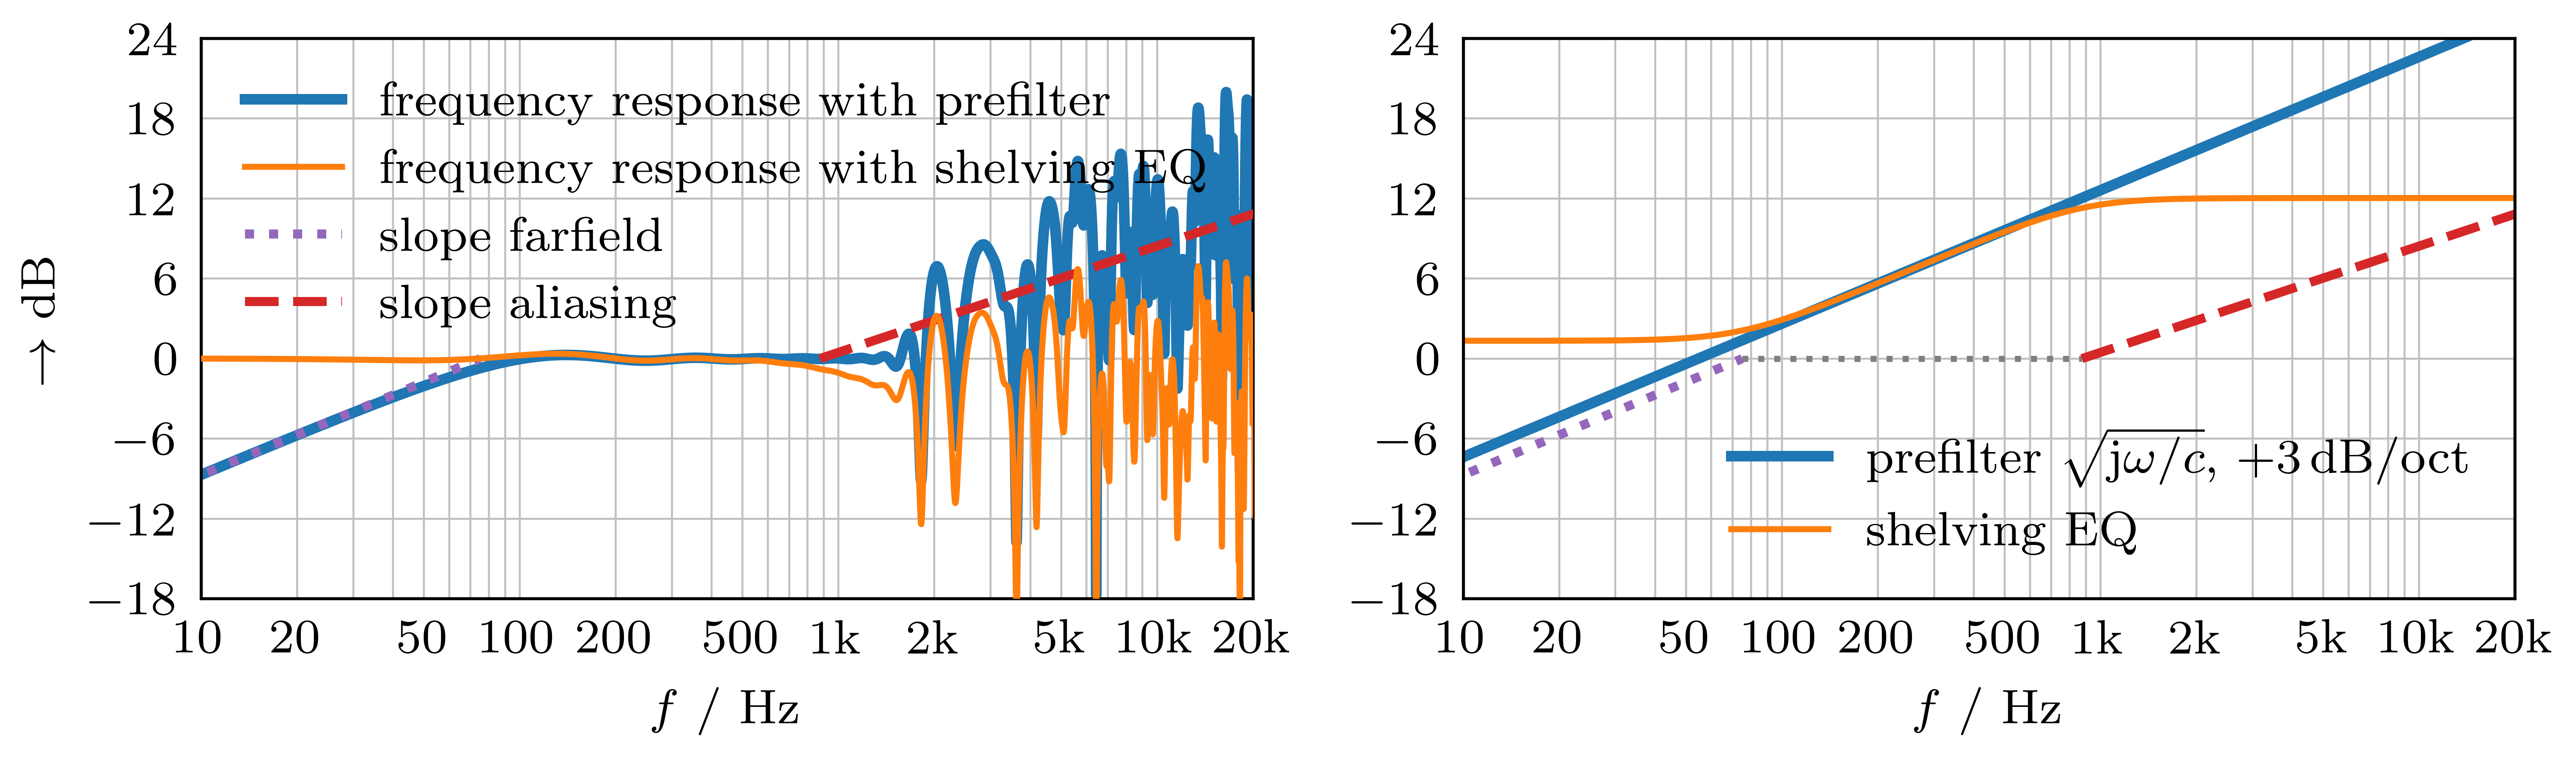
\includegraphics[width=174mm]{../python/wfs25d_lineSSD_aliasing_eq_example_ENG.png}
\end{plotfigures}
\caption{%2.5D-WFS-Szenario ähnlich \myfig\ref{fig:wfs25d_circSSD_aliasing} aber
%mit Kreisarray bestehend aus 64 Monopolen. Messpunkt $\xr = (0,0,0)^\mathrm{T}$\,m.
2.5D WFS of a virtual point source.
Measurement point at $\xr = (0,0,0)^\mathrm{T}$\,m.
The setup is similar to that of \myfig\ref{fig:td_0m}
but uses a circular array with 64 monopoles instead of 32.
This doubles the spatial aliasing frequency.
%
%Frequenzgang (links, blau) unter Benutzung des theoretischen WFS-Vorfilters
%$\sqrt{\im \omega/c}$ (rechts, blau).
Frequency response (left, blue) using the theoretical WFS prefilter
$\sqrt{\im \omega/c}$ (right, blue).
%
%Dieser gemessene Frequenzgang weist zwei charakteristische Flanken mit
%ca. $+3$\,dB/Oktave auf.
This measured frequency response exhibits two characteristic slopes
of approximately $+3$\,dB/octave.
%
%Die tieffrequente Flanke in lila erklärt sich vor allem
%durch ein zu wenig ausgeprägtes Nahfeld des Arrays (Apertur kleiner als Wellenlänge).
The low-frequency slope, shown in purple, is primarily due to an
insufficiently pronounced near field of the array,
i.e. the aperture is smaller than the wavelengths.
%
%Die hochfrequente Flanke in rot erklärt sich durch den zu großen Abstand der
%Monopole im Array (räumliches Aliasing).
The high-frequency slope, shown in red, is caused by the
inappropriately large loudspeaker spacing, i.e. by spatial aliasing.
%
%Linearisierter Frequenzgang (links, orange) unter Benutzung eines
%Shelving-WFS-Vorfilters (rechts, orange).
Linearised frequency response (left, orange) due to the usage of the adapted
WFS shelving prefilter (right, orange).
%
%Die Shelving-Plateaus des Filters resultieren in einer tief- bzw. hochfrequenten
%Anhebung bzw. Absenkung im Vergleich zum theoretischen WFS-Vorfilter.
The shelving filter's plateaus result in a level boost/cut
for the low/high frequency region, compared with the theoretical
WFS prefilter.
%
%Dies führt zu einer Linearisierung des Frequenzgangs für den gewählten Messpunkt.
This results in a linearisation of the frequency response for the
selected measurement point.
%
\cc
}
\label{fig:wfs25d_lineSSD_aliasing_eq_example}
\end{figure*}



%Eine sehr einfache Entzerrungsmethodik, welche bei der impliziten
%Schallfeldsyntheselösung streng genommen nur einen einzelnen Empfängerpunkt
%linearisiert, besteht in der Modifikation des globalen WFS-Vorfilters.
One simple method involves modifying the theoretical
WFS prefilter\index{WFS prefilter} to linearise the frequency response
of a single receiver point.
%
%Dies ist beispielhaft in
%\myfig\ref{fig:wfs25d_lineSSD_aliasing_eq_example} gezeigt.
This is illustrated in \myfig\ref{fig:wfs25d_lineSSD_aliasing_eq_example}.
%
%Dafür wurde das 2.5D-WFS-Szenario aus \myfig\ref{fig:wfs25d_circSSD_aliasing}
%verwendet, jedoch mit einem Kreisarray mit 64 Monopolen, wovon 23 aktiv sind.
The 2.5D WFS scenario from \myfig\ref{fig:td_0m} was
used for this purpose, but with a circular array of 64 monopoles, 23 of which
are active.
%
%Die Kreisbogenlänge zwischen zwei Monopolen beträgt ca. $0{,}2$\,m.
The arc length between two adjacent monopoles is approximately $0{.}2$\,m.
%
%Der gewählte Messpunkt $\xr = (0,0,0)^\mathrm{T}$\,m liegt auf der
%Referenzkurve und ist Teil eines Punktpaars stationärer Phase.
The selected measurement point $\xr = (0,0,0)^\mathrm{T}$\,m belongs to a
stationary phase point pair and is part of the amplitude-corrected
reference curve.
%
%Im Idealfall ist für diesen Messpunkt also ein linearer $0$\,dB-Frequenzgang
%zu erwarten.
Ideally, a flat, $0$\,dB frequency response can be expected for
this probe point.
%
%In der linken Grafik in \myfig\ref{fig:wfs25d_lineSSD_aliasing_eq_example}
%ist der resultierende Frequenzgang in blau dargestellt.
The resulting frequency response is shown in blue in the left diagram
of \myfig\ref{fig:wfs25d_lineSSD_aliasing_eq_example}.
%
%Er weist zwei charakteristische $+3$\,dB/Oktave Flanken auf.
It has two characteristic slopes of $+3$\,dB/octave.
%
%Die tieffrequente Flanke (lila) stellt das bereits diskutierte Hochpassverhalten
%dar.
The purple line represents the high-pass behaviour that has already
been discussed.
%
%Die hochfrequente Flanke (rot) entspricht dem mittleren Pegelanstieg
%durch zunehmende Ausprägung räumlichen Aliasings.
The red dashed line shows the high-frequency slope.
This average increase in level is due to an increase in spatial aliasing.
%
%Da die charakteristischen (Anti)-Resonanzen stark abhängig von der
%Messposition sind, lässt sich nur der mittlere Pegelanstieg sinnvoll entzerren.
Since these characteristic (anti)-resonances are highly dependent
on the measurement position, only the average increase of the level
can be effectively equalised.



%Die beiden charakteristischen Flanken lassen sich mit gegenläufigen Flanken
%kompensieren.
The two characteristic slopes can be compensated for by opposing slopes.
%
%Die Reihenschaltung des theoretischen WFS-Vorfilters aus
%der \myeq\eqref{eq:Prefilter25D} mit dem Kompensationsfilter ergibt ein für den
%gewählten Messpunkt adaptiertes WFS-Vorfilter.
Cascading the theoretical WFS prefilter from \myeq\eqref{eq:Prefilter25D}
in series with the compensation filter results in a WFS prefilter adapted
to the selected measurement point.
%
%Es hat die Form eines Shelving-Filters mit $+3$\,dB/Oktave ansteigender Flanke.
This is a shelving filter with a rising slope of $+3$\,dB/octave.
%
%Das Filter sollte einfach zu parametrisieren sein, da a) das WFS-Setup,
%b) die Primärquellenparametrik und c) der Messpunkt einen Einfluss auf die untere
%und obere Flanken-Eckfrequenz haben.
The filter should be easy to parametrise, since the lower and upper
cut-off frequencies are affected by the WFS setup, the parameters
of the virtual source, and the measurement point.
%
%Diese sollten sinnvollerweise nach technischen und/oder perzeptiven
%Optimierungskriterien festgelegt werden.
The cut-off frequencies should be determined according to technical
and/or perceptual optimisation criteria.
%
%Im Beispiel wurde das Entwurfsverfahren für Shelving-Filter aus \cite{Schultz2020a}
%verwendet.
The design procedure for shelving filters from \cite{Schultz2020a}
was used for this example.
%
%Die obere Grenzfrequenz $f_\text{o}=f_\text{max} \approx 873$\,Hz wurde
%nach dem Kriterium in \myeq\eqref{eq:SamplingCriterion} festgelegt.
The upper cut-off frequency $f_\text{U}=f_\text{max} \approx 873$\,Hz
was set according to the criterion in \myeq\eqref{eq:SamplingCriterion}.
%
%Um den Frequenzgang am Messpunkt tieffrequent auf $\approx 0$\,dB-Pegel zu
%kompensieren wurde die untere Grenzfrequenz $f_\text{u}=75$\,Hz
%gewählt.
A lower cut-off frequency of $f_\text{L}=75$\,Hz was manually chosen to
compensate for the low-frequency level, bringing it to approximately $0$\,dB.
%
%Der Shelving-Filter-Frequenzgang weist im Frequenzbereich $f_\text{u} < f < f_\text{o}$
%die gewünschte $+3$\,dB/Oktave Flanke ähnlich des theoretischen WFS-Vorfilters auf,
%vgl.~\myfig\ref{fig:wfs25d_lineSSD_aliasing_eq_example}~(rechts).
The frequency response of the shelving filter exhibits a $+3$\,dB/octave slope
in the frequency range $f_\text{L} < f < f_\text{U}$,
which is similar to that of the theoretical WFS prefilter,
cf.~\myfig\ref{fig:wfs25d_lineSSD_aliasing_eq_example}~(right).
%
%Für $f<f_\text{u}$ und $f>f_\text{o}$ wird der Verlauf des
%theoretischen WFS-Vorfilters (blau) begrenzt und führt so zum adaptierten
%Shelving-WFS-Vorfilter (orange).
For $f<f_\text{L}$ and $f>f_\text{U}$ the frequency response of the
theoretical WFS prefilter (blue) is thus flattened, resulting in an adapted
shelving WFS prefilter (orange).
%
%Diese Begrenzung führt zum linearisierten Frequenzgang für den gewählten Messpunkt,
%links dargestellt in \myfig\ref{fig:wfs25d_lineSSD_aliasing_eq_example} in orange.
This adjustment produces a linearised frequency response at the selected
measurement point, shown in orange on the left
in \myfig\ref{fig:wfs25d_lineSSD_aliasing_eq_example}.



%\subsection{WFS mit numerischer Optimierung}
\subsection{WFS with Numerical Optimisation}

%Das im vorherigen Unterabschnitt beschriebene Verfahren folgt dem
%Paradigma Audiosignal-Vorfilterung, Verzögerung und Verstärkung gemäß des
%Signalflusses in \myfig\ref{fig:WFS_Blockdiagramm}.
The procedure described in the previous subsection adheres
to the prefiltering, delaying and amplitude-scaling paradigm of audio
signals, as shown in \myfig\ref{fig:WFS_Blockdiagramm}.
%
%Es wurden WFS-Adaptionen diskutiert, welche dieses Paradigma zugunsten einer
%lautsprecherindividuellen Filterung aufgeben.
WFS adaptations that deviate from this paradigm in favour
of loudspeaker-specific filtering are known in the literature.
%
%Damit kann das Schallfeld für die jeweils gewünschte akustische Szene optimiert
%werden, typisch die Minimierung von frequenzabhängigen
%Beugungs- und Aliasingartefakten für einen relevanten -- meist groß intendierten
% -- Zuhörerbereich.
This allows the sound field to be optimised for the desired acoustic scene.
Typically, frequency-dependent diffraction and spatial aliasing artefacts
are minimised for a relevant listening area.
%
%Erwähnenswert sind hier die numerischen Optimierungen
%von WFS-Referenzschallfeldern \cite{Gauthier2006_JASA,Gauthier2007_JAES,Corteel2006_JAES}.
The numerical optimisation of WFS reference sound fields
according to
\cite{Gauthier2006_JASA,Gauthier2007_JAES,Corteel2006_JAES}
are worth mentioning here.
%
%Diese Methoden erfordern umfangreiche Simulation und/oder Messung der
%Referenzschallfelder.
These methods require simulations and/or measurements
of the reference sound fields.
%
%Pro Lautsprecher wird dann ein zusätzliches Filter
%mit endlicher Impulsantwort (FIR-Filter) benötigt, damit frequenzabhängig
%Einfluss auf Delay und Gain genommen werden kann.
Additional filtering using a finite impulse response (FIR) filter
is then required for each loudspeaker signal to adjust
the frequency-dependent group delay and gain.
%
%Im WFS-Signalflussgraphen \myfig\ref{fig:WFS_Blockdiagramm} ist dieses zusätzliche
%FIR-Filter optional nachgeschaltet.
\myfig\ref{fig:WFS_Blockdiagramm} shows the optional FIR filter stage
at the end of the electrical signal chain.



%Erwähnenswert ist, dass die numerische Optimierung von 2.5D-Schallfeldproblemen
%nicht über physikalisch gesetzte Grenzen hinausgehen kann, d.h.
%die 2.5D-inhärente Amplitudencharakteristik lässt sich mit Numerik nicht
%kompensieren, sondern sollte vielmehr Bestandteil des Optimierungsziels sein.
It is worth noting that the numerical optimisation of 2.5D sound field
problems cannot overcome physical limitations.
This means that the inherent amplitude function of 2.5D cannot be
compensated for.
Instead, it should be included as part of the optimisation target.



%\subsection{Lokale WFS}
\subsection{Local WFS}

%Die Anwendung von WFS mit Optimierung für einen sehr
%begrenzten, kleineren Zuhörerbereich wird in der Literatur als sogenannte
%lokale WFS geführt.
In the literature, the application of WFS with optimisation for a very
limited listening area is referred to as local WFS.
%
%Ihr Forschungsschwerpunkt ist die Erzeugung kleiner, aliasing-reduzierter
%Schallfeldzonen \cite{Corteel2008_AES}, in letzter Zeit vorangetrieben zu
%(halb)-analytischen Lösungen des lokalen Schallfeldsyntheseproblems vor allem für
%kreisförmige Lautsprecherarrays \cite{Winter2019_diss,Hahn2019,Hahn2022_JAES}.
The research focuses on the generation of small, spatial-aliasing-reduced sound
field zones \cite{Corteel2008_AES}.
Recently, (semi)-analytical solutions to the local sound field synthesis
problem have been advanced, particularly for circular loudspeaker arrays,
cf. \cite{Winter2019_diss,Hahn2019,Hahn2022_JAES}.
%
%Grundidee der lokalen Verfahren ist eine räumliche Bandbegrenzung der Ansteuerung,
%was lautsprecherindividuelle FIR-Filterung erfordert,
%die alle Lautsprecher betrifft, im Gegensatz zur \textit{secondary source selection}
%bei nicht-lokaler WFS.
The basic idea behind local WFS is to modify the spectrum and restrict the
spatial bandwidth of the driving functions.
Thus, FIR filtering is required for each loudspeaker signal.
In contrast to non-local WFS, all loudspeakers are active.



% please DO NOT rescale the figure and keep it double column
\begin{figure*}
\centering
\begin{plotfigures}
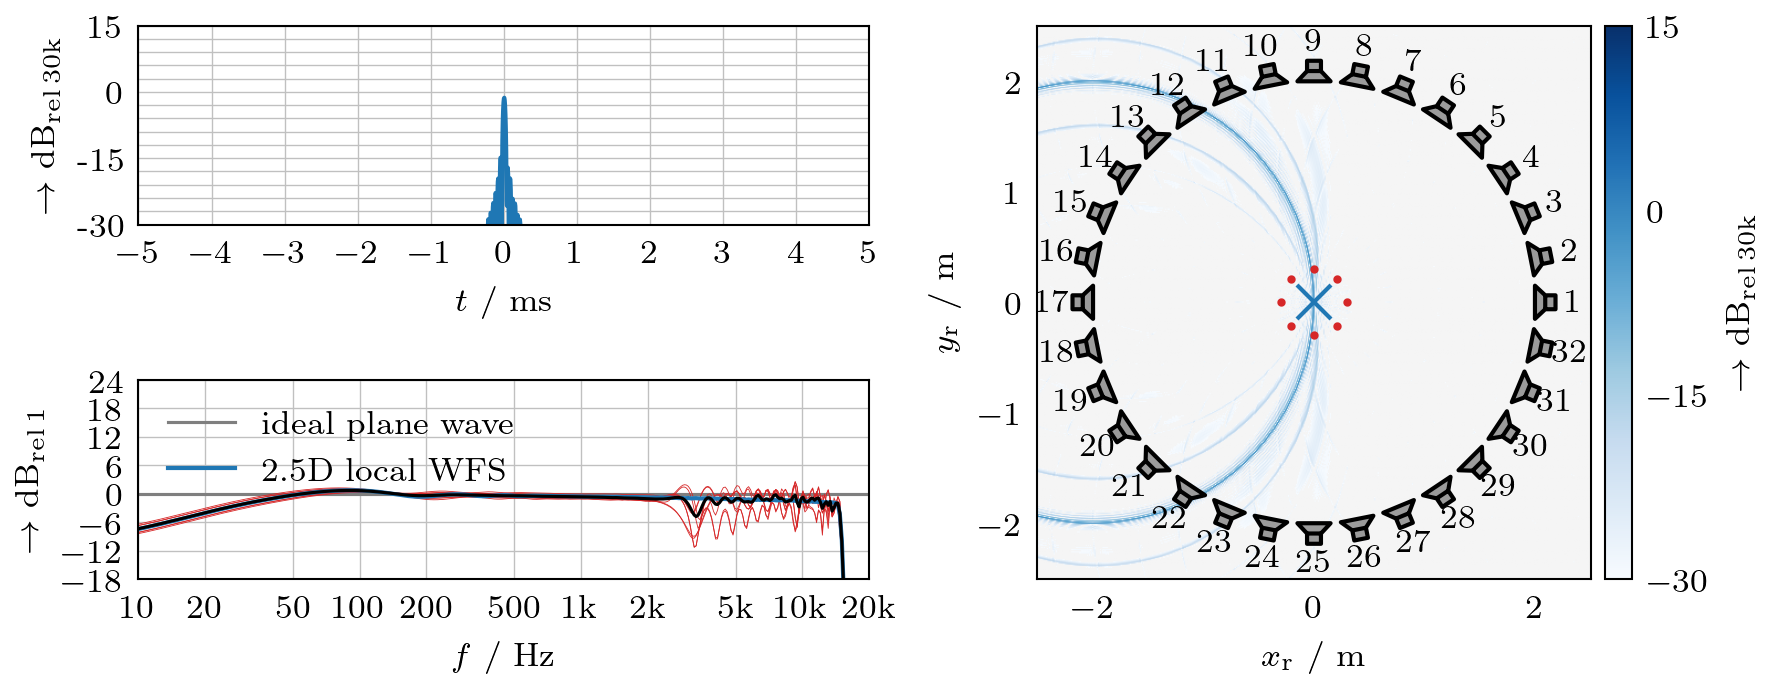
\includegraphics[width=145mm]{../python/lwfs25d_circSSD_time_domain_center_py_ENG.png}
\end{plotfigures}
\caption{%2.5D lokale WFS einer lokal planaren, impulshaften
%Wellenfront mit Ausbreitung in Richtung positiver $x$-Achse optimiert
%für den Referenzpunkt $\times$ bei $\xr=(0,0,0)^\mathrm{T}$\,m.
2.5D local WFS of a locally planar, impulsive wavefront propagating
in the direction of the positive $x$-axis,
optimised for the reference point $\times$ at $\xr=(0,0,0)^\mathrm{T}$\,m.
%
%Wellendurchlauf am Referenzpunkt $\times$ zum gewählten Zeitbezug $t=0$\,s.
Wave passage at the reference point $\times$ occurs at the here defined
time reference $t=0$\,s.
%
%Gleiches Setup wie in \myfig\ref{fig:td_0m}; bei lokaler WFS sind alle Lautsprecher
%aktiv; Benutzung des idealen 2.5D-WFS-Vorfilters \eqref{eq:Prefilter25D};
%
Same setup as in \myfig\ref{fig:td_0m}; all loudspeakers are active
for local WFS;
usage of the theoretical 2.5D WFS prefilter \eqref{eq:Prefilter25D};
%
%Abtastfrequenz $f_s=192$ kHz;
%
%Ordnungen für
%sphärische Harmonische,
%zylindrische Harmonische,
%Lagrange-Polynom,
%Fourier-Reihe:
orders for spherical harmonics, cylindrical harmonics, Lagrange polynomials,
and Fourier series:
$N=30$, $M_s=15$, $\mathcal{M}=5$, $M_a=20$;
%und Kaiser-Bessel-Fenster mit $\beta=6$.
Kaiser-Bessel window with $\beta=6$.
%
%Im Vergleich zu WFS erzeugt lokale WFS im Referenzpunkt wegen weniger
%räumlicher Aliasingartefakte einen linearen Frequenzgang über größeren
%Frequenzbereich und eine zeitlich kompaktere Impulsantwort.
Local WFS produces a linear frequency response across a broader
frequency range and a temporally more compact impulse response
at the reference point than non-local WFS, due to the reduced occurrence
of spatial aliasing artefacts.
%
%Frequenzgänge in rot für die rot markierten Messpunkte auf dem Radius $0{,}3$\,m weisen
%größere Verzerrungen wegen zeitlich weniger kompakten Impulsantworten auf.
The frequency responses for the red-marked measurement points at a radius
of $0{.}3$\,m show greater distortion due to temporally less compact
impulse responses.
%
%Energetisch gemittelter Frequenzgang aus allen Messpunkten in schwarz.
The energetically averaged frequency response of all the measurement
points is shown in black.
%
\cc
}
\label{fig:td_lwfs_center}
\end{figure*}



%\myfig\ref{fig:td_lwfs_center} und \ref{fig:td_lwfs_offcenter} zeigen Ergebnisse
%des lokalen WFS-Verfahrens nach \cite{Hahn2022_JAES} erneut mit dem Kreisarray aus
%32 Lautsprechern auf 2 m Radius.
The \myfigs\ref{fig:td_lwfs_center} and \ref{fig:td_lwfs_offcenter} show the
results of the local WFS method according to \cite{Hahn2022_JAES},
again using the circular array of 32 loudspeakers with a radius of $2$\,m.
%
%Im jeweilig gewählten Referenzpunkt,
%d.h. im optimalen Zentrum der für die lokale WFS berücksichtigten Schallfeldzone,
%wird räumliches Aliasing vollständig vermieden.
Spatial aliasing is completely avoided at the chosen reference point,
which is the optimal centre of the sound field zone considered for
the local WFS.
%
%Die Synthese der impulshaften, lokal ebenen Wellenfront gelingt in diesem Messpunkt
%artefaktfrei, weil die Interferenzen exakt auf dieses Ergebnis hin
%kontrolliert werden, d.h. die räumliche Bandbegrenzung ist dafür optimiert.
At this measurement point, the locally planar wavefront is synthesised
without artefacts because the interferences are precisely aligned.
The spatial bandwidth limitation is optimised for this purpose.
%
%Dies widerspiegelt sowohl die zeitlich kompakte Impulsantwort mit einem
%symmetrischen Peak zum gewählten Referenzzeitpunkt als auch der lineare Frequenzgang
%in blau.
This is reflected in both the compact impulse response, which features
a symmetrical peak shape at the selected reference time, and in the
flat frequency response, shown in blue.
%
%In unmittelbarer Nähe des Referenzpunktes, z.B. bei den rot dargestellten Messpunkten
%in $0{,}3$\,m Abstand, sind die Interferenzen nicht mehr perfekt zueinander abgestimmt.
In the immediate vicinity of the reference point -- for example, at the red
measurement points located $0{.}3$\,m away -- the interferences are no longer
perfectly aligned.
%
%Daher resultieren Artefakte von räumlichem Aliasing und räumlicher Bandbegrenzung
%in den roten Frequenzgängen
This results in artefacts caused by spatial aliasing and spatial bandwidth
limitation, shown in the red frequency responses.
%; diese
%Verzerrungen sind deutlich geringer als bei nicht-lokaler WFS in den
%\myfig\ref{fig:td_-1m} bis \ref{fig:td_1m}.
However, these artefacts are considerably less pronounced than those
observed with non-local WFS in the \myfigs\ref{fig:td_-1m}--\ref{fig:td_1m}.
%
%Der energetisch gemittelte Frequenzgang in schwarz kann als weitgehend linear
%aufgefasst werden.
The energetically averaged frequency responses, in the
\myfigs\ref{fig:td_lwfs_center} and \ref{fig:td_lwfs_offcenter} shown in black,
are largely flat.
%
%Die lokale WFS erzeugt in diesem Beispiel also kopfgrößere, lokale
%Schallfeldzonen mit vergleichsweise wenig Klangverfärbung.
Hence, in this example, the local WFS produces local sound field zones
with little sound colouration, which are slightly larger than
the human head.



% please DO NOT rescale the figure and keep it double column
\begin{figure*}
\centering
\begin{plotfigures}
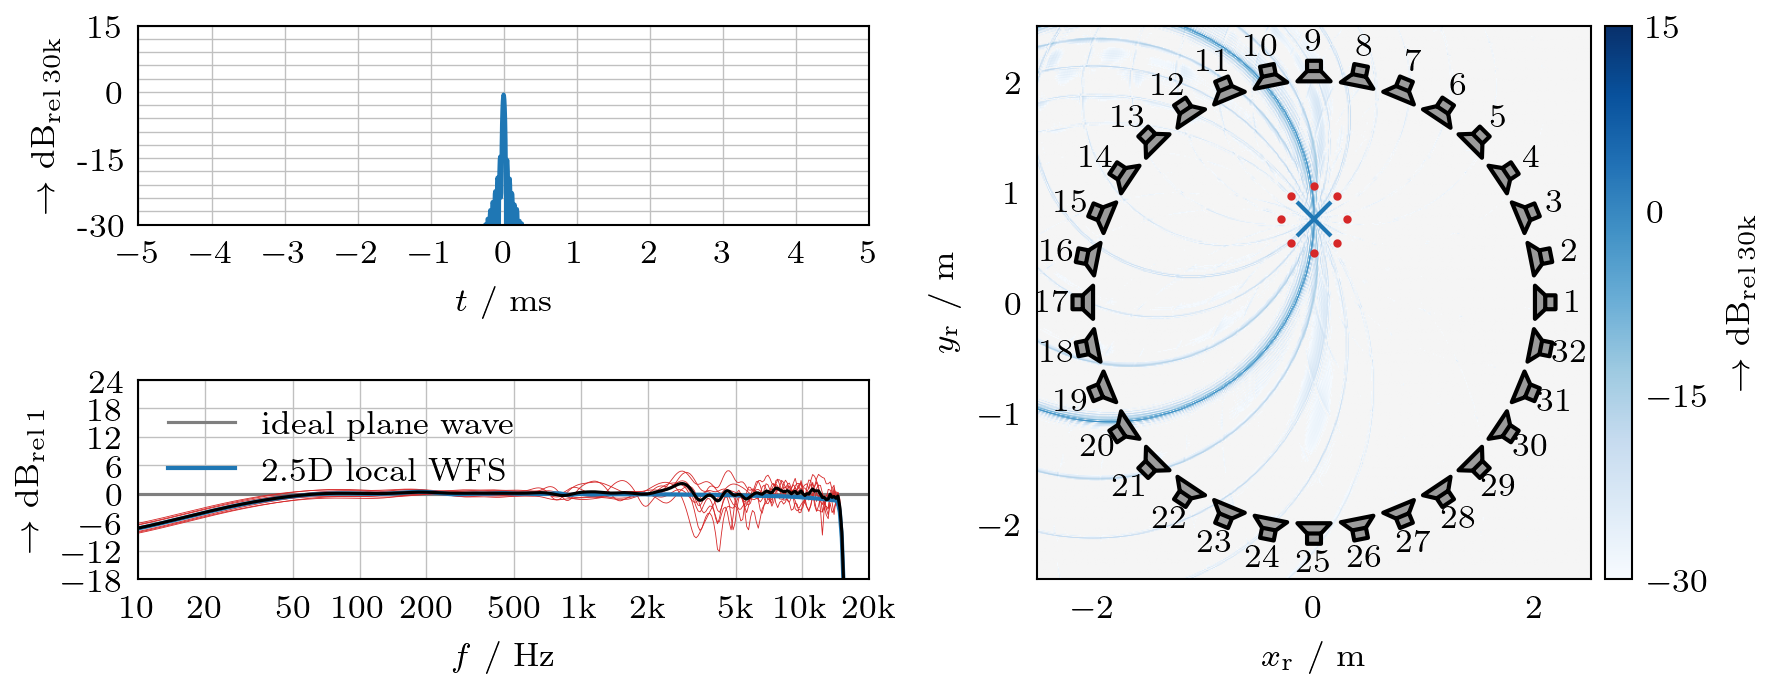
\includegraphics[width=145mm]{../python/lwfs25d_circSSD_time_domain_offcenter_py_ENG.png}
\end{plotfigures}
\caption{%2.5D lokale WFS optimiert für den Referenzpunkt
%$\times$ bei $\xr=(0,\frac{3}{4},0)^\mathrm{T}$\,m, sonst wie \myfig\ref{fig:td_lwfs_center}.
2.5D local WFS optimised for reference point
$\times$ at $\xr=(0,\frac{3}{4},0)^\mathrm{T}$\,m,
otherwise as \myfig\ref{fig:td_lwfs_center}.
%
\cc
}
\label{fig:td_lwfs_offcenter}
\end{figure*}



%\section{Werkzeuge}
\section{Tools}
%\label{sec:WFS_Werkzeuge}
\label{sec:WFS_tools}

%WFS-Ansteuerungsalgorithmen für objektorientiertes 3D-Audio mit
%echtzeitfähigem Rendering finden sich unter anderem in den folgenden Software-Projekten
Control algorithms for WFS-based, object-oriented 3D audio with real-time
rendering capabilities can be found in the following software projects,
among others:
\begin{itemize}
\item \cite{url:wonder}, \cite{url:wonder_lite} offspring of the WFS software
which was initially developed at TU Berlin  %wonder, Standalone\\\url{https://github.com/dvzrv/wonder}
%\item \cite{url:wonder_lite} %wonder-lite, Standalone\\\url{https://github.com/ntonnaett/wonder}
\item \cite{url:ssr} % Sound Scape Renderer, Standalone\\\url{https://github.com/SoundScapeRenderer}
\item \cite{url:iem-wfs} as VST plugin
\item \cite{url:wfscollider} for SuperCollider %WFSCollider für SuperCollider\\\url{https://github.com/GameOfLife/WFSCollider}
\item \cite{url:wfs-diy} for Max %Wave Field Synthesis DIY für Max %\\\url{https://wfs-diy.net/}
\item \cite{Belloch2016_IEEE} for WFS rendering on GPUs
\end{itemize}
%
%Kommerzielle, teils hardware-gebundene Lösungen für WFS sind unter anderem
Commercial solutions for the WFS, some of which are hardware-based,
and some with presumably proprietary WFS algorithm extensions, include:
\begin{itemize}
\item \cite{url:panoramix} stand-alone software for post-production
\item \cite{url:spat_revolution} for Max %IRCAM SPAT Revolution für Max\\\url{https://forum.ircam.fr/projects/detail/spat/}
\item \cite{url:flux_spat_revolution}, optional WFS license; stand-alone,
or AAX-, AU-, VST-plugins, or with an option for live sound production,
such as for digital mixing consoles %Flux Spat Revolution Ultimate mit Live Production Option, für Digitalmischpulte\\\url{https://www.flux.audio/project/spat-revolution/}
\item \cite{url:iosono} %\& Spatial Audio Workstation %IOSONO inside \& Spatial Audio Workstation\\\url{https://encircled-audio.com/}
\item \cite{url:amadeus_holophonix} (use of IRCAM SPAT algorithms) %Amadeus HOLOPHONIX (benutzt IRCAM SPAT Technologie)\\\url{http://holophonix.xyz/}
\item \cite{url:holoplot} %Holoplot\\\url{https://holoplot.com/}
\end{itemize}
%mit mutmaßlich proprietären WFS-Algorithmikerweiterungen.



%Sowohl die Benutzerfreundlichkeit,
%konsistente Produktionsarbeitsabläufe als auch planare Lautsprecherpanele,
%welche mittels Audio-Netzwerken angesteuert werden \cite{Reussner2013_JAES},
%vgl. Holoplot, gewinnen an Bedeutung beim Einsatz von WFS für 3D-Beschallungsszenarien.
User-friendliness, consistent production workflows and planar loudspeaker
panels controlled by audio networks, cf. \cite{Reussner2013_JAES}
and the approach by the company Holoplot,
are becoming increasingly important in the use of WFS for 3D sound reinforcement
scenarios.
%
%Stand frühe 2020er Jahre scheinen Ambisonics, kanal- und objektbasierter Surround Sound,
%sowie kopfhörerbasierte Binauraltechnik
%die der WFS bevorzugten 3D-Wiedergabe-Verfahren zu sein.
As of the 2020s, Ambisonics, channel- and object-based surround sound,
and headphone-based binaural technology appear to be the preferred 3D audio
playback methods.
%
%Es ist zu erwarten, dass vermehrt hybride Systeme mit 3D-Ambisonics und 2.5D-~bzw.~3D-WFS
%zum Einsatz kommen, um beide Ansätze sinnvoll zu ergänzen.
It is reasonable to hypothesise that hybrid systems incorporating 3D Ambisonics
and 2.5D/3D WFS will be increasingly utilised to complement both approaches in
a meaningful way.



%\vspace{\baselineskip}Alle Grafiken dieses Kapitels sind in \cite{SchultzHahnSpors2025}
%unter CC BY 4.0 Lizenz verfügbar.
\vspace{\baselineskip}All graphics in this chapter are available
in \cite{SchultzHahnSpors2025} and can be reused under the CC BY 4.0 license.
